\documentclass[11pt,rightpage,a4paper]{memoir}
\usepackage{mathtools,amsthm,amssymb,amsfonts,geometry,multicol,pifont,eufrak, mathrsfs}
\usepackage{mleftright, hyperref}
\usepackage[dvipsnames]{xcolor}
\usepackage{pgfplots,enumerate}


\usetikzlibrary{arrows}
\usetikzlibrary{patterns}
\usepgfplotslibrary{fillbetween}
\pgfplotsset{compat=1.4}

\semiisopage % Print placement in page
\chapterstyle{hangnum} % Chapter heading style


%\newtheoremstyle{thm}{\topsep}{\topsep}{\itshape}{}{\bfseries}{}{\newline}{}
\newtheoremstyle{problems}{\topsep}{\topsep}{}{}{\bfseries}{}{\newline}{}
\theoremstyle{thm}
\newtheorem{thm}{Theorem}[section]
\newtheorem{defn}[thm]{Definition}
\newtheorem{notation}[thm]{Notation}
\newtheorem{rmk}[thm]{Remark}
\newtheorem{fact}[thm]{Fact}
\newtheorem{ex}[thm]{Example}
\theoremstyle{problems}
\newtheorem{prblm}[thm]{}

\colorlet{shadecolor}{gray!10}
\newenvironment{pblm}
   {\begin{shaded}\begin{prblm}}
   {\end{prblm}\end{shaded}}

\title{Real Analysis Notebook}
\author{Mary Barker}
\date{Spring 2017}


\newcommand{\Q}{\mathbb{Q}}
\newcommand{\R}{\mathbb{R}}
\newcommand{\C}{\mathbb{R}}
\newcommand{\M}{\mathfrak{M}}
\newcommand{\Sp}{\mathscr{P}}
\newcommand{\Z}{\mathbb{Z}}
\newcommand{\Zp}{\mathbb{Z}^+}
\newcommand{\Dp}{\dot{+}}
\newcommand{\A}{\mathfrak{A}}
\newcommand{\B}{\mathfrak{B}}
\newcommand{\mDref}[1]{Definition \ref{#1}}
\newcommand{\mPref}[1]{\# \ref{#1}}

\begin{document}
	\begin{titlingpage}
		\maketitle
	\end{titlingpage}

	\chapter{Preliminaries}
\begin{defn}\label{d:finite}%1
A set $A$ is \textbf{finite} if there is a 1-1 mapping of some set $\{1, 2, 3, ..., n\}$ 
of positive integers onto $A$. $A$ is \textbf{countably infinite} if there is a 1-1 
mapping of the set $\Zp$ of positive integers onto $A$. $A$ is \textbf{countable} 
if either finite or countably infinite. Otherwise $A$ is \textbf{uncountable}. 
\end{defn}

\begin{pblm}%2
	(deMorgan laws) If $\{E_\lambda: \lambda \in \Lambda\}$ is any indexed collection of 
	subsets of some set $E$, then 
	\begin{equation*}
		\left(\bigcup\limits_{\lambda \in \Lambda} E_\lambda\right)^c = 
		\bigcap\limits_{\lambda \in \Lambda} E_\lambda^c ~~~ \text{ and }~~~
		\left(\bigcap\limits_{\lambda \in \Lambda} E_\lambda\right)^c = 
		\bigcup\limits_{\lambda \in \Lambda} E_\lambda^c 
	\end{equation*}
	where $A^c$ denotes the complement of $A$ in $E$. 
\begin{proof}
	\begin{equation*}
	\left(\bigcup\limits_{\lambda \in \Lambda} E_\lambda\right)^c = 
	\{x: x \in E_\lambda \text{ for some } \lambda \in \Lambda\}^c = 
	\{x: x \in E_\lambda^c \forall \lambda \in \Lambda\} = 
	\bigcap\limits_{\lambda \in \Lambda} E_\lambda^c
	\end{equation*}
	\begin{equation*}
	\left(\bigcup\limits_{\lambda \in \Lambda} E_\lambda\right)^c = 
	\{x: x \in E_\lambda \text{ for some } \lambda \in \Lambda\}^c = 
	\{x: x \in E_\lambda^c \forall \lambda \in \Lambda\} = 
	\bigcap\limits_{\lambda \in \Lambda} E_\lambda^c
	\end{equation*}
\end{proof}
\end{pblm}

\begin{rmk}%3
	In the previous problem the index set $\Lambda$ need not be countable. One could 
	imagine indexing a collection of sets by the real numbers, for instance (e.g. 
	$E_x$ is the interval of length 1 centered at $x$.)
\end{rmk}

\pagebreak
\begin{pblm}%4
	Any countable union of sets of real numbers can be expressed as a disjoint 
	union: $E \cup F = E \cup (F \setminus E)$ or $\bigcup\limits_{k = 1}^\infty 
	E_k = \bigcup\limits_{k = 1}^\infty F_k$ where $F_1 = E_1$, 
	$F_k = E_k \setminus \bigcup \limits_{j = 1}^{k - 1} E_j$. Here $A \setminus B = 
	A \cap B^c$. 
\begin{proof}
	Let $E, F$ be sets of real numbers. 
	Then for any $x \in E \cup F$, if $x \in E$, then 
	$x \in E \subset \{E \cup (F \setminus E)\}$. Similarly, if $x \notin E$ but 
	$x \in F$, then $x \in (F \setminus E) \subset \{E \cup (F \setminus E)\}$. 
	Thus 
	\begin{equation*}
		E \cup F ~\subset~ E \cup (F\setminus E). 
	\end{equation*}

	On the other hand, for any $x \in E \cup (F \setminus E)$, if $x \in E$ then 
	$x \in E \cup F$. Also, if $x \in F \setminus E$ then $x \in F \subset (E \cup F)$. 
	Thus 
	\begin{equation*}
		E \cup (F \setminus E) \subset E \cup F. 
	\end{equation*}

	\begin{equation*}
		E \cup F ~ \substack{\subset \\ \supset}~ E \cup (F \setminus E) ~~~\implies~~~
		E \cup F = E \cup (F \setminus E).
	\end{equation*}

	For the more general case, take any $x \in \bigcup\limits_{j=1}^\infty F_k$, then there is some $F_j$ such that 
	$x \in F_j$. Since each $F_j \subset E_j$, then 
	$x \in E_j \subset \bigcup\limits_{j=1}^\infty E_j$. Therefore 
	$\bigcup\limits_{j=1}^\infty F_j\subset \bigcup\limits_{j=1}^\infty E_j$. 

	On the other hand, for any $x \in \bigcup\limits_{j=1}^\infty E_j$. Then there is 
	some $k$ such that $x \in E_k$. Let $a$ be the 
	smallest index such that $x \in E_a$. Then $x \in E_a$ and $\forall b < a$, $x 
	\notin E_b$. Therefore $x \in F_a$, and so $x \in \bigcup\limits_{j=1}^\infty F_j$. 
	Therefore, since we have shown subset containment in both directions, 

	\begin{equation*}
		\bigcup\limits_{j=1}^\infty E_j = \bigcup\limits_{j=1}^\infty F_j. 
	\end{equation*}
\end{proof}
\end{pblm}

\begin{pblm}%5
	If $a$ and $b$ are real numbers, then $a \le b$ iff for every $\epsilon > 0$, 
	$a \le b + \epsilon$. Similarly, $a \ge b$ iff for every $\epsilon > 0$, 
	$a \ge b - \epsilon$. 
\begin{proof}
	Let $a, b \in \R$ and $a \le b$. Then for every $\epsilon > 0$, 
	$a \le b < b + \epsilon$, and therefore $a \le b + \epsilon$. 
	Now, let $a, b \in \R$, and assume that for any 
	$\epsilon > 0$, $a \le b + \epsilon$. Then if $a > b$, there is some 
	$\epsilon_1 \ge 0$ such that $a = b + \epsilon_1$. But since $a \le b + \epsilon$ for 
	all $\epsilon > 0$, we have 
	$a \le b + \frac{\epsilon}{2} < b + \epsilon_1 = a $ 
	which is a contradiction. Therefore $a \le b$. 

	Now let $a \ge b$. This can be re-written as $b \le a$. By 
	the first part of the problem, $b \le a$ iff $\forall \epsilon > 0$, 
	$b \le a + \epsilon$. This is true iff $b - \epsilon \le a$. 
\end{proof}
\end{pblm}

\begin{rmk}%6
	This problem may seem trivial, but we will use it over and over again during the quarter. 
	It says that we can give a little something away, and then take it back. 
\end{rmk}

\begin{defn}\label{d:boundedset}%7
~
	\begin{enumerate}[(a)]
		\item A set $E$ of real numbers is \textbf{bounded above} if there 
		exists a real number $u$ such that for every $x \in E$, $x \le u$. 
		we call $u$ an \textbf{upper bound} for $E$. Similarly, $E$ is 
		\textbf{bounded below} if there exists a real number $w$ such that 
		for every $x \in E$, $w \le x$, and then $w$ is a \textbf{lower bound} 
		for $E$. $E$ is \textbf{bounded}, if bounded both above and below. 
		\item If $E$ is bounded above and nonempty, the \textbf{supremum} 
		(or least upper bound) of $E$, sup $E$, is the unique real number $s$ 
		such that (i) $s$ is an upper bound for $E$ and (ii) $s < u$ for any 
		other upper bound $u$ for $E$. Similarly, if $E$ is bounded below 
		and nonempty, the \textbf{infimum} (or greatest lower bound) of $E$, 
		inf $E$, is the unique real number $t$ such that (i) $t$ is a lower 
		bound for $E$ and (ii) $t > w$ for any other lower bound $w$ for $E$. 
		(Recall that the Least Upper Bound Axiom guarantees the existence of 
		the supremum and infimum.) 
		\item A real number $c$ is a \textbf{cluster point} of a set $E$ of 
		real numbers if for every $\epsilon > 0$ there is $y \in E$ such that 
		$0 < |c - y| < \epsilon$. 
	\end{enumerate}
\end{defn}

\begin{pblm}%8
	Let $v$ be a lower bound for a set $E$ of real numbers, where $v \notin E$. Then 
	$v = \inf E$ iff $v$ is a cluster point of $E$. 
\begin{proof}
	Let $v = \inf E$, $v \notin E$. Then for any $\epsilon > 0$, 
	there is $y \in E$ such that $y < v + \epsilon$, as otherwise $v + \epsilon$ would 
	be a lower bound of $E$ greater than $v = \inf E$. Now, for any $\epsilon > 0$, we 
	have $y \in E$ such that 
	\begin{equation*}
		v < y < v + \epsilon
	\end{equation*}
	Subtracting $v$ from each inequality, this can be re-written as 
	\begin{equation*}
		0 < y - v < \epsilon
	\end{equation*}
	and since $y > v$, this is 
	\begin{equation*}
		0 < |y - v| < \epsilon ~~~ \Leftrightarrow ~~~ 0 < |v - y| < \epsilon 
	\end{equation*}
	Thus $v$ is a cluster point of $E$. 

	Now, assume that $v$ is a cluster point of $E$, $v \notin E$, and $v$ is a L.B. for 
	$E$. 

	For any $w > v$, $w = v + \epsilon$ for some $\epsilon > 0$, there is $y \in E$ such that 
	$v < y < v + \epsilon$. Therefore $w$ is not a lower bound of $E$. Thus $v = \inf E$. 
\end{proof}
\end{pblm}

\pagebreak
\begin{defn}\label{d:boundedsequence}%9
	~
	\begin{enumerate}[(a)]
		\item A \textbf{sequence} of real numbers $\{a_k\}_{k=1}^\infty$ is 
		a function from the set of positive integers $\Zp$ into the 
		real numbers. (More generally, the domain of a sequence can be any set 
		of the form $\{k: k \ge k_0\}$ for some integer $k_0$.) The sequence is 
		\textbf{bounded} (or bounded above or ... ) if its range is bounded 
		(or ... ).
		\item The sequence $\{a_k\}_{k = 1}^\infty$ \textbf{converges} to the 
		\textbf{limit} $a$ if for each $\epsilon > 0$ there is a positive 
		integer $K$ such that $|a_k - a| < \epsilon$ for all $k \ge K$. 
		\item A \textbf{subsequence} $\{a_{k_j}\}_{j = 1}^\infty$ of a 
		sequence $\{a_k\}_{k = 1}^\infty$ is the composition of 
		$\{a_k\}_{k = 1}^\infty$ with an increasing sequence 
		$\{k_j\}_{j = 1}^\infty$ of integers 
	\end{enumerate}
\end{defn}

\begin{pblm}%10
	Let $\{a_k\}_{k = 1}^\infty$ be a non-decreasing sequence of real numbers. Then 
	$\{a_k\}_{k = 1}^\infty$ is bounded above iff $\{a_k\}_{k = 1}^\infty$ converges
	to the least upper bound of the set $\{a_k : k \in \Zp\}$. (Of course 
	there is a symmetric result for non-increasing sequences.)
\begin{proof}
	Let $\{a_k\}_{k=1}^\infty$ be bounded above. Now, let $L$ be the least upper bound of 
	the set $\{a_k: k \in \Zp\}$. Since $\{a_k\}$ is a non-decreasing sequence, 
	for each $ k \in \Zp$, $a_k \le a_{k + 1} \le a_{k + 2} \le ... $ 
	And also, for all $k \in \Zp$, $a_k \le L$ since $L$ is the least upper bound. 
	Therefore for all $k \in \Zp$, 
	\begin{equation*}
		a_k \le a_{k + 1} \le \cdots \le L
	\end{equation*}
	For any $\epsilon > 0$, let $a^\ast = L - \epsilon < L$. Then since $L$ is the least 
	upper bound of the set $\{a_k: k \in \Zp\}$, we know that $a^\ast \le a_j$ for 
	some $j \in \Zp$. Therefore (using the fact that the sequence is 
	non-decreasing) for all $k \ge j$, 
	\begin{equation*}
		L \ge a_k \ge L - \epsilon 
	\end{equation*}
	which can be re-written as 
	\begin{equation*}
		0 \le |L - a_k| \le \epsilon
	\end{equation*}
	Thus $\{a_k\}_{k=1}^\infty$ converges to the least upper bound 
	

	Now, if $\{a_k\}_{k=1}^\infty$ converges to the L.U.B $L$ of $\{a_k:k\in\Zp\}$
	and $a_k \le a_{k+1}$ for all $k \in \Zp$, then for all $k \in \Zp$, 
	we have 
	\begin{equation*}
		a_k \le a_{k + 1} \le \cdots \le L 
	\end{equation*}
	Thus $\{a_k\}_{k = 1}^\infty$ is bounded above. 
\end{proof}
\end{pblm}

\pagebreak
\begin{rmk}%11
~
\begin{enumerate}
	\item Note the distinction between the sequence $\{a_k\}_{k = 1}^\infty$, which 
	as a function is a set of ordered pairs of real numbers, and the set 
	$\{a_k: k \in \Zp\} \subset \R$ which is the range of that 
	function. 
	\item If $\{a_k\}_{k = 1}^\infty$ is non-decreasing and not bounded above, 
	we often write $\lim\limits_{k\to\infty} a_k = \infty$ and speak as though 
	$\infty$ were a number ``way out there at the end of the number line.'' We do 
	not, however, do arithmetic with $\infty$. 
\end{enumerate}
\end{rmk}

\begin{defn}\label{d:convergesequence}%12
~
\begin{enumerate}
	\item $\{a_k\}_{k = 1}^\infty$ be a sequence of real numbers. The numbers 
	$s_n = \sum\limits_{k = 1}^n a_k$ are the \textbf{partial sums of the infinite 
	series} $\sum\limits_{k = 1}^\infty a_k$. The series \textbf{converges} if 
	$\lim\limits_{n\to\infty}s_n$ exists (as a real number). Otherwise the series 
	\textbf{diverges}. If the series converges, the number $s = \lim\limits_{n\to\infty}
	s_n$ is called the \textbf{sum of the infinite series} and is denoted 
	$\sum\limits_{k = 1}^\infty a_k$. 
	\item More generally, if $S$ is any set of positive integers, and for any 
	positive integer $n$, $S_n = \{k \in \Zp:k\in S \text{ and }k\le n\}$, 
	we define the finite sums $s_n = \sum\limits_{k \in S_n} a_k$ to be the 
	\textbf{partial sums} of the series $\sum\limits_{k \in S}a_k$, and say that 
	the series \textbf{converges} if $\lim\limits_{n\to\infty}s_n$ exists (as a 
	real number). Otherwise the series \textbf{diverges}. If the series converges, 
	the number $s = \lim\limits_{n\to\infty}s_n$ is called the \textbf{sum of the 
	series} and is denoted $\sum\limits_{k \in S}a_k$. 
\end{enumerate}
\end{defn}

\begin{pblm}%13
	Let $\{a_k\}_{k = 1}^\infty$ be a sequence of non-negative reals. Let 
	$\{F_j\}_{j = 1}^\infty$ be any nested sequence of sets of positive integers 
	such that $F_1 \subset F_2 \subset ...$ and $\bigcup\limits_{j = 1}^\infty F_j 
	= \Zp$. For each $j$ let $f_j = \sum\limits_{k \in F_j} a_k$. Then 
	$\sup_j f_j = \sum\limits_{k = 1}^\infty a_k$. (This means that if either 
	number is finite, then they both are and and then they are equal. Notice 
	that it is not assumed that the sets $F_j$ are finite, so the $f_j$ need not 
	be finite.)\\
	%\textbf{Remark}: This is a strong form of saying that a series with non-negative 
	%terms can be summed in any order without affecting the sum. 
\begin{proof}

$\sum\limits_{k=1}^\infty a_k = \sum\limits_{k \in \cup_{j=1}^\infty F_j}a_k \in \{f_j\}_{j=1}^\infty$
And so, by definition 
\begin{equation*}
	\sum\limits_{k=1}^\infty a_k ~~\le~~ \sup_j f_j
\end{equation*}

Now, since $\forall j \in \Zp$, $F_j \subset F_{j+1}$, then 
\begin{equation*}
f_j = \sum\limits_{k \in F_j}a_k \le \sum\limits_{k\in F_{j+1}} a_k = f_{j+1}
\end{equation*}
Now, if the $F_j$ are finite, then 
using the fact that $\{f_j\}_{j=1}^\infty$ is a sequence of non-decreasing positive 
real values, we have 
\begin{equation*}
	f_j = \sum\limits_{k\in F_j}a_k \le \lim\limits_{n\to\infty}f_n = \sum\limits_{k=1}^\infty a_k ~~~ \forall j \in \Zp
\end{equation*}
On the other hand, if the $F_j$ are not necessarily finite, the values can be re-ordered in 
increasing order, and then each $f_j$ can be written 
as the limit of a sequence of partial sums 
$\lim\limits_{n\to\infty}\sum\limits_{k=1}^n a_{j(k)}$ 
where $F_j = \{j(k)\}_{k=1}^\infty$. Then all of the partial sums are bounded above by 
$\sum\limits_{k=1}^\infty a_k$, and so $f_j \le \sum\limits_{k=1}^\infty a_k$ for all $j$ 
and irrespective whether the $F_j$ are finite or infinite. 

Therefore $\sum\limits_{k=1}^\infty a_k$ is an upper bound of $\{f_j\}_{j=1}^\infty$, and so 
\begin{equation*}
	\sup_j f_j \le \sum\limits_{k\in F_j}a_k 
\end{equation*}
\end{proof}
\end{pblm}

\begin{pblm}%14
	Consider the double indexed set $\{a_{j,k}\}_{j,k=1}^\infty$ of non-negative 
	numbers. Set $S_n = \sum\limits_{j,k=1}^na_{j,k}$. (This means the sum of the 
	$n^2$ terms $a_{j,k}$ where $1 \le j \le n$ and $1 \le k \le n$.) Let 
	$A_1 = \lim\limits_{n\to\infty}S_n$, 
	$A_2 = \sum\limits_{j=1}^\infty \sum\limits_{k=1}^\infty a_{j,k}$, 
	$A_3 = \sum\limits_{k=1}^\infty \sum\limits_{j=1}^\infty a_{j,k}$. 
	Then $A_1=A_2=A_3$. This means that if any 
	one of these three numbers is finite, then all of them are and they are 
	equal. (This is, of course, the equivalent for series of the fact that a 
	double integral can be evaluated as an iterated integral. For instance, $A_2$ 
	if it exists, is the limit as $n \to \infty$ of 
	$\sum\limits_{j=1}^\infty\sum\limits_{k=1}^\infty a_{j,k}$.)
\begin{proof}
	Now, as a sum of non-negative numbers for any $n$,
	\begin{equation*}
		S_n = \sum\limits_{j=1}^n\sum\limits_{k=1}^na_{j,k}\le
		\sum\limits_{j=1}^\infty\sum\limits_{k=1}^\infty a_{j,k}=A_2
	\end{equation*}
	which implies that, since this is true for any $n$, $A_1 \le A_2$. 

	Now to show that $A_2 \le A_1$, we will consider the sequence 
	$\{T_n\}_{n=1}^\infty = \{\sum\limits_{j=1}^n\sum\limits_{k=1}^\infty a_{j,k}\}_{n=1}^\infty$. This is a 
	sequence of non-decreasing positive values with $\lim\limits_{n\to\infty}T_n = A_2$. 
	Also for all $n \in \Zp$, 
	\begin{equation*}
		\sum\limits_{j=1}^n\sum\limits_{k=1}^\infty a_{j,k} \le A_1
	\end{equation*}
	And so $A_2 \le A_1$. 

	Note that $S_n = \sum\limits_{j=1}^n\sum\limits_{k=1}^na_{j,k}=\sum\limits_{k=1}^n\sum\limits_{j=1}^na_{j,k}$
	As a finite sum, and that, since this is true for all $n$, then showing that $A_1 = A_2$ is equivalent to 
	showing $A_1 = A_3$

\end{proof}
\end{pblm}

\begin{defn}%15
~
	\begin{enumerate}[(a)]
		\item An \textbf{open ball} about a real number $x$ of radius $r$ 
		is the set $B_r(x) = (x - r, x + r)$. 
		\item A set $G$ of real numbers is \textbf{open} if it contains an 
		open ball about each of its points. 
		\item A set $F$ of real numbers is \textbf{closed} if every cluster 
		point of $F$ is contained in $F$. 
	\end{enumerate}
\end{defn}

\begin{pblm}%16
	Every open subset $G$ of real numbers can be expressed as a countable union 
	of pairwise disjoint open intervals. (Think about the rationals in $G$.)
\begin{proof}
Consider all of the the rational numbers in $G$. This is a countable set, so 
indexing by any subset of this set will also be countable. 

Now, for all rational $x \in G$, let $I_x$ be the largest open interval in $G$ containing 
$x$. For any $y \in G$ such that $y$ is not rational, Because $G$ is open, we can find 
$\epsilon > 0$ such that $y \in (x - \epsilon, x + \epsilon)\subset G$ for some rational 
$x \in G$. Then the set $\{I_x : x \in G \text{ is rational} \}$ is an open cover of $G$. 

To find a subset that are pairwise disjoint and that covers all of $G$, consider any two 
rational numbers $x, y \in G$. If $I_x \cap I_y \neq \emptyset$, then by the maximality 
of $I_x$ and $I_y$ $x \in I_x \cup I_y \subset G$, and so $I_x = I_x \cup I_y = I_y$. 
Thus every pair of intervals
$I_x, I_y$ is either disjoint or identical intervals. 
\end{proof}
\end{pblm}

\begin{defn}\label{d:compact}%17
	The set $E$ of real numbers is \textbf{compact} if every sequence 
	$\{a_k\}_{k=1}^\infty$ of elements of $E$ has a subsequence that converges 
	to an element of $E$. 
\end{defn}

\begin{fact}%18
	These properties are equivalent for a set $E$ of real numbers. 
	\begin{enumerate}[(a)]
		\item $E$ is compact. 
		\item $E$ is closed and bounded. 
		\item Every infinite subset of $E$ has a cluster point in $E$. 
		\item If $\{G_\lambda: \lambda \in \Lambda\}$ is a collection of open 
		sets such that $E \subset \bigcup\limits_{\lambda \in \Lambda}G_\lambda$ 
		(an \textbf{open cover} of $E$), then some finite subcollection is 
		also an open cover of $E$.
	\end{enumerate}
\end{fact}




	\chapter{Measure on $[0, 1]$}

\begin{defn}\label{d:outermeasure}%19
	For any subset $E$ of $[0,1]$, the \textbf{outer measure} 
	of $E$ is 
	\begin{equation*}
		m^\ast(E) = \inf\left\{\sum\limits_{j=1}^\infty \ell(G_j) 
		: E \subset \bigcup\limits_{j=1}^\infty G_j\right\}
	\end{equation*}
	where each $G_j = (a_j,b_j)$ is an open interval in $\R$ and 
	$\ell(G_j) = b_j - a_j$. (Note: this includes finite sums by 
	setting all $G_j = \emptyset$ from some point on. Also note the $G_j$ 
	need not be contained in $[0,1]$, e.g. in considering $m^\ast(\{1\})$). 
\end{defn}

\begin{rmk}~ %20
	\begin{enumerate}[(a)]
		\item We could use coverings by closed intervals and get the same 
		result. It is clear that we could get numbers not larger than we 
		have. (Replace $G_j = (a_j, b_j)$ by $F_j = [a_j, b_j]$.) To 
		see not smaller, replace closed $F_j$ by open $G_j$ where 
		$\ell(G_j) = \ell(F_j) + \epsilon / 2^j$. 
		\item There is also something called inner measure. But it is not 
		needed, so we won't use it. 
	\end{enumerate}
\end{rmk}

\begin{pblm}%21
	For any subset $E$ of $[0,1]$, 
	\begin{enumerate}[(a)]
		\item $0 \le m^\ast(E) \le 1$.
		\item $E \subset F \Rightarrow m^\ast(E) \le m^\ast(F)$. 
		\item $m^\ast(\emptyset) = m^\ast(\text{one point})=0$.
	\end{enumerate}
\begin{proof}
~
\begin{enumerate}[(a)]
	\item For any $\epsilon > 0$, consider the open interval $(-\frac{\epsilon}{2}, 1 + \frac{\epsilon}{2})$ 
	that has length $1 + \epsilon$. This is an open cover of $[0,1]$, and so it is also an open 
	cover of $E \subset [0,1]$. Now, since $\epsilon$ was arbitrarily chosen, $m^\ast(E) \le 1$. 

	Also, since $m^\ast(E)$ is the infimum of a set of non-negative numbers, $m^\ast(E) \ge 0$. 

	So $0\le m^\ast(E)\le 1$ for all $E \subset [0,1]$. 

	\item Let $H=\left\{\sum\limits_{j=1}^\infty\ell(G_j):F\subset\bigcup\limits_{j=1}^\infty G_j\right\}$  
	and let $G=\left\{\sum\limits_{j=1}^\infty\ell(G_j):E\subset\bigcup\limits_{j=1}^\infty G_j\right\}$. 
	Since $E\subset F$, we know that $H\subset G$. Therefore $\inf(G)\le\inf(H)$. 

	\item For any $x \in [0,1]$, consider $(x - \epsilon / 2, x + \epsilon / 2)$ for any 
	$\epsilon > 0$. This is an open cover of $\{x\}$ with length $\epsilon$. Using the 
	fact that $\epsilon$ was arbitrarily chosen, the infimum of sums of lengths of intervals 
	must be less than or equal to $\epsilon$, which implies that $m^\ast(\{x\}) \le 0$. 

	Now, since $\emptyset \subset \{x\}$, we can use part (b), which gives 
	$m^\ast(\emptyset) \le m^\ast(\{x\}) \le 0$. 
\end{enumerate}
\end{proof}
\end{pblm}

\begin{pblm}%22
	If $E$ is a countable set, then $m^\ast(E) = 0$. In particular, 
	$m^\ast(\Q_0) = 0$ where $\Q_0 = \Q \cap [0,1]$ 
	is the set of all rational numbers in $[0,1]$.

 	(Given $\epsilon > 0$ cover $E = \{x_k\}_{k=1}^\infty$ with 
	$\bigcup\limits_{j=1}^\infty G_j$ where $\ell(G_j) = \epsilon / 2^j$.)
\begin{proof}
	Suppose $E$ is countable. Then we can write $E = \{x_i\}_{i=1}^\infty$. Then 
	for any $\epsilon > 0$, define $G_i = (x_i - \frac{\epsilon}{2^{i+1}}, x_i + \frac{\epsilon}{2^{i+1}})$. 
	Then $\ell(G_i) = 2\frac{\epsilon}{2^{i+1}}=\frac{\epsilon}{2^i}$. 
	Therefore $\bigcup\limits_{i=1}^\infty G_i$ is an open cover of $E$, and 
	\begin{equation*}
		\sum\limits_{i=1}^\infty\ell(G_i) = \sum\limits_{i=1}^\infty\frac{\epsilon}{2^i} = \epsilon. 
	\end{equation*}
	Therefore 
	\begin{equation*}
		m^\ast(E)\le\inf\left\{\sum\limits_{i=1}^\infty\ell(G_i):E\subset\bigcup\limits_{i=1}^\infty G_i\right\} = 0. 
	\end{equation*}
	and so $m^\ast(E) = 0$. 
\end{proof}
\end{pblm}

\begin{rmk}%23
	This is the first evidence that covering $E$ with countably infinite 
	unions rather than finite unions makes a big difference. This is, in 
	fact exactly the innovation that will allow us to deal much more 
	efficiently with infinite processes and with irregular sets. 
\end{rmk}

\begin{pblm}%24
	If $F = [a,b]$ is a closed interval in $[0,1]$, then $m^\ast(F)=b-a$. 
	($m^\ast(F) \le b - a$ is clear from $G = (a - \epsilon, b + \epsilon)$. 
	$F$ is compact, so any cover has a finite subcover $\bigcup\limits_{j=1}^n
	G_j$. May assume that no element of this subcover can be omitted (Explain 
	why.) Order them by their left endpoints and show $\sum\limits_{j=1}^n 
	\ell(G_j) > b - a.$)
\begin{proof}
	First we will show that $m^\ast(F) \le (b - a)$ and then that $m^\ast(F) \ge (b-a)$. 

	Now, $m^\ast(F) = \inf\left\{\sum\limits_{j=1}^\infty\ell(G_j):F\subset\bigcup\limits_{j=1}^\infty G_j\right\}$, and 
	so if we consider an arbitrary open cover $\{G_j\}_{j=1}^\infty$ of $F$, 
	$m^\ast(F) \le \sum\limits_{j=1}^\infty\ell(G_j)$. 
	In particular, Let us consider the open cover $(a - \epsilon / 2, b + \epsilon / 2)$ for 
	any $\epsilon > 0$. This has length $ (b - a) + \epsilon$. Thus 
	$m^\ast(F) \le (b - a) + \epsilon$ for all $\epsilon > 0$, and so 
	\begin{equation*}
		m^\ast(F) \le b - a
	\end{equation*}

	Now, let $\{G_j\}_{j = 1}^n$ be any finite subcover of $F$. Then if there are 
	$G_k = (a_k, b_k), G_l = (a_l, b_l) \in [0,1]$ such that $G_k \subset G_l$, 
	then we can throw out $G_k$. 

	Thus we can remove all extraneous $G_k$, and so if we reorder the elements 
	of $\{G_j\}_{j=1}^n$ in increasing order such that $a_0 < a $ and $b < b_n$. 
	With the increasing order for all $j$, $a_j < a_{j+1}$ and 
	$a_{j+1} < b_j < b_{j+1}$, since otherwise we would have 
	$(a_j,b_j) \subset (a_{j+1},b_{j+1})$. Then
	\begin{equation*}
		\sum\limits_{j=1}^n\ell(G_j) = \sum\limits_{j=1}^n (b_j-a_j)
	\end{equation*}
	This can be re-written as 
	\begin{equation*}
		\sum\limits_{j=1}^n(b_j-a_j) = (b_n - a_1) + (b_{n-1} - a_n) + (b_{n-2} - a_{n-1}) + \cdots
	\end{equation*}
	Now, since for all $j$, $b_j > a_{j+1}$, this is 
	\begin{equation*}
		b_n - a_1 + \epsilon
	\end{equation*}
	for some $\epsilon > 0$. Now, since $b = b_n + \epsilon_b$ and 
	$a_1 = a - \epsilon_b$ for some $\epsilon_a, \epsilon_b  > 0$, 
	we have 
	\begin{equation*}
		b_n + a_1 + \epsilon \ge b_n + a_1 = b - a + (\epsilon_b + \epsilon_a) \ge b - a. 
	\end{equation*}
	Continuing this with $\sum\limits_{j=1}^n\ell(G_j)$, we end with 
	\begin{equation*}
		\sum\limits_{j=1}^n \ell(G_j) \ge b - a
	\end{equation*}

	Since this open cover was arbitrarily chosen, $(b - a)$ is a lower bound, which means that since $m^\ast(F)$ is 
	the infimum, 
	\begin{equation*}
		m^\ast(F) = \inf\left\{\sum\limits_{j=1}^\infty\ell(G_j):F\subset\sum\limits_{j=1}^\infty G_j\right\} \ge (b - a)
	\end{equation*}
\end{proof}
\end{pblm}

\begin{pblm}%25
	If $E,F \subset [0,1]$, $m^\ast(E\cup F) \le m^\ast(E) + m^\ast(F)$. 
\begin{proof}
	Since the outer measure of any set $m^\ast$ is an infimum, it is a cluster 
	point. Therefore for any $\epsilon > 0$, there are open covers $\{G_j\}_{j=1}^\infty$ 
	and $\{H_j\}_{j=1}^\infty$ such that 
	\begin{equation*}
		\sum\limits_{j=1}^\infty\ell(G_j) = m^\ast(E) + \frac{\epsilon}{2} ~~~\text{ and }~~~ 
		\sum\limits_{j=1}^\infty\ell(H_j) = m^\ast(F) + \frac{\epsilon}{2}
	\end{equation*}
	Now, since $E \subset \bigcup\limits_{j=1}^\infty G_j$ and $F \subset \bigcup\limits_{j=1}^\infty H_j$, 
	$ E \cup F \subset \left(\bigcup\limits_{j=1}^\infty G_j\right) \cup \left(\bigcup\limits_{j=1}^\infty H_j\right)$ 
	and so 
	\begin{equation*}
		\begin{array}{rcccl}
			m^\ast(E \cup F) & \le & \sum\limits_{j=1}^\infty\ell(G_j) + \sum\limits_{j=1}^\infty\ell(H_j) 
					& = & m^\ast(E) + \frac{\epsilon}{2} + m^\ast(F) + \frac{\epsilon}{2}\\
					& & & = & m^\ast(E) + m^\ast(F) + \epsilon
		\end{array}
	\end{equation*}
	Thus $m^\ast(E\cup F) \le m^\ast(E) + m^\ast(F)$. 
\end{proof}
\end{pblm}

\begin{pblm}%26
	For any subsets $\{E_j\}_{j=1}^\infty$ of $[0,1]$, 
	$m^\ast\left(\bigcup\limits_{j=1}^\infty E_j\right) \le 
	\sum\limits_{j=1}^\infty m^\ast (E_j).$
	We refer to this property of outer measure as 
	\textbf{countable subadditivity}.
\begin{proof}
	Note that for any set of open covers of all of the $E_j$ is an open cover of $\cup E_j$. That is, for 
	$\left\{ \{I_{j_k}\}_{k=1}^\infty: E_j \subset \bigcup\limits_{k=1}^\infty I_{j_k}\right\}$, 
	$\bigcup\limits_{j=1}^\infty E_j \subset \bigcup\limits_{j=1}^\infty\bigcup\limits_{k=1}^\infty I_{j_k}.$ 

	For any $\{E_j\}_{j=1}^\infty$, consider any open covers $\{I_{j_k}\}_{k=1}^\infty$ 
	of each $E_j$. Then since each $m^\ast(E_j)$ is a cluster point, then for any $\epsilon > 0$ 
	there is $\{I_{j_k}\}_{k=1}^\infty$ such that 
	\begin{equation*}
		\sum\limits_{k=1}^\infty \ell(I_{j_k}) \le m^\ast(E_j) + \frac{\epsilon}{2^j}
	\end{equation*}
	And so for any $\epsilon > 0$, we can choose open covers of each of the $E_j$ such that 
	\begin{equation*}
		m^\ast\left(\bigcup\limits_{j=1}^\infty E_j\right) \le 
		\sum\limits_{j=1}^\infty\sum\limits_{k=1}^\infty \ell(I_{j_k}) \le 
		\sum\limits_{j=1}^\infty \left(m^\ast(E_j)+ \frac{\epsilon}{2^j}\right) = 
		\sum\limits_{j=1}^\infty m^\ast(E_j) + \epsilon
	\end{equation*}
	Therefore by (5), 
	\begin{equation*}
		m^\ast\left(\bigcup\limits_{j=1}^\infty E_j\right) \le \sum\limits_{j=1}^\infty m^\ast(E_j)
	\end{equation*}
\end{proof}
\end{pblm}

\begin{defn}\label{d:measurable}%27
	A subset $E$ of $[0,1]$ is \textbf{measurable} if for 
	each $A \subset [0,1]$, 
	\begin{equation*}
		m^\ast(A) = m^\ast(A\cap E) + m^\ast(A\cap E^c). 
	\end{equation*}
\end{defn}

\begin{notation}%28
	If $E$ is measurable, we write $m(E)$ for $m^\ast(E)$ and refer to 
	this number as the \textbf{Lebesgue measure} of $E$. 
\end{notation}

\begin{rmk}~ %29
	\begin{enumerate}[(a)]
		\item From the previous problem, to show that $E$ is measurable 
		one need only prove 
		$m^\ast(A) \ge m^\ast(A\cap E) + m^\ast(A\cap E^c)$ since the other 
		direction is automatic. 
		\item In particular, taking $A = [0,1], 1 = m^\ast(E)+m^\ast(E^c)$ 
		is a necessary condition for measurability. It turns out that this 
		special case of the definition is also sufficient. The definition 
		is the way it is (rather than this simpler version) just because 
		it is a little more convenient to use.
	\end{enumerate}
\end{rmk}

\begin{pblm}%30
{\color{gray!10}{thing}}
\begin{enumerate}[(a)]
	\item $\emptyset$ is measurable. $[0,1]$ is measurable.
	\item $m^\ast(E) = 0 \Rightarrow E$ is measurable. 
\end{enumerate}
\begin{proof}
{\color{gray!10}{thing}}
\begin{enumerate}[(a)]
	\item In $[0,1]$, $\emptyset^c = [0,1]$, and $[0,1]^c = \emptyset$. Therefore 
	for any $A \subset [0,1]$, 
	\begin{equation*}
		\begin{array}{rcccl}
		m^\ast(A) & = & m^\ast(A \cap [0,1]) & = & m^\ast(A \cap [0,1]) + 0\\
			 & = & m^\ast(A \cap [0,1]) + m^\ast(\emptyset) & = & m^\ast(A \cap [0,1]) + m^\ast(A \cap \emptyset)
		\end{array}
	\end{equation*}
	Thus $[0,1]$ is measurable. 
	Similarly, 
	\begin{equation*}
		\begin{array}{rcl}
		m^\ast(A) & = & 0 + m^\ast(A \cap [0,1])\\
			 & = & m^\ast(\emptyset)         + m^\ast(A \cap [0,1]) \\
			 & = & m^\ast(A \cap \emptyset)  + m^\ast(A \cap [0,1]) 
		\end{array}
	\end{equation*}
	Thus $\emptyset$ is measurable. 
	\item If $m^\ast(E) = 0$, then for any set $A$, $A \cap E \subset E$, and 
	since $A \cap E^c \subset A$, we have (by 21 (b)): 
	\begin{equation*}
		\begin{array}{rcl}
		m^\ast(A\cap E^c) & \le & m^\ast (A)\\
		0 + m^\ast(A\cap E^c) & \le & m^\ast (A)\\
		m^\ast(A \cap E) + m^\ast(A\cap E^c) & \le & m^\ast (A)
		\end{array}
	\end{equation*}
	Therefore, using the observation in 29(a), $E$ is measurable. 
\end{enumerate}
\end{proof}
\end{pblm}

\begin{rmk}%31
	In particular, every subset of a set of outer measure 0 is measurable. 
\end{rmk}

\begin{pblm}%32
	$E$ is measurable $\Leftrightarrow E^c$ is measurable. 
\begin{proof}
\begin{equation*}
	\begin{array}{rcl}
	E ~\text{ is measurable }~ & \Leftrightarrow & ~ \forall A \subset [0,1], m^\ast(A) = m^\ast(A \cap E) + m^\ast(A \cap E^c)\\
				& \Leftrightarrow & ~ \forall A \subset [0,1], m^\ast(A) = m^\ast(A \cap E^c) + m^\ast(A \cap E)\\
				& \Leftrightarrow & ~ \forall A \subset [0,1], m^\ast(A) = m^\ast(A \cap E^c) + m^\ast(A \cap (E^c)^c)\\
				& \Leftrightarrow & E^c ~\text{ is measurable}
	\end{array}
\end{equation*}
\end{proof}
\end{pblm}

\begin{pblm}%33
	A closed interval $[a,b]$ is measurable with measure $b-a$. 

	(Show $m^\ast(A) \ge m^\ast(A\cap[a,b])+m^\ast(A\cap[a,b]^c)-\epsilon$ 
	for every $\epsilon$. If $\bigcup\limits_{j=1}^\infty G_j$ covers $A$ 
	with $\bigcup\limits_{j=1}^\infty \ell(G_j)$ near $m^\ast(A)$, then the 
	$G_j\cap[a,b]$ are nearly an open cover of $A\cap[a,b]$ by open intervals 
	and similarly for $G_j\cap[a,b]^c$.)
\vspace{.25cm}

\begin{proof}
	Let $A \subset [0,1]$. Then 
	for any $\epsilon > 0$, choose an open cover $\{G_j\}_{j=1}^\infty$ of $A$ 
	such that $\sum\limits_{j=1}^\infty \ell(G_j) \le m^\ast(A) + \frac{\epsilon}{2}$. 

	Define $F_1 = \left\{G_k \cap (a, b) \right\}
		\cup (a-\frac{\epsilon}{8},a+\frac{\epsilon}{8})
		\cup (b-\frac{\epsilon}{8},b+\frac{\epsilon}{8})$, 
	$F_2 = \left\{G_k \cap [a, b]^c\right\}$, 

	Then $A \cap [a, b] \subset F_1$ and $A \cap [a, b]^c \subset F_2$. 
	(note that the elements of $F_2$ are either open intervals or else 
	sets of the form $(x, a) \cup (b, y)$ for some $x, y \in \R$.
	Therefore the notion of length is still well-defined on $F_2$ and $F_2$ 
	is still a collection of open intervals, and thus an open cover) 

	Since $\{O: O \subset F_1\}$ is an open cover of $A \cap [a, b]$ and 
	$\{O: O \subset F_2\}$ is an open cover of $A \cap [a, b]^c$, 
	Therefore, 
	$m^\ast(A \cap [a,b]) \le \sum\limits_{O \in F_1}\ell(O)$ and 
	$m^\ast(A \cap [a,b]^c) \le \sum\limits_{O \in F_2}\ell(O)$. 
	Also, since the only intersection of $F_1$ and $F_2$ is in the 
	$(a - \frac{\epsilon}{8}, a + \frac{\epsilon}{8})$, $(b - \frac{\epsilon}{8}, b + \frac{\epsilon}{8})$ 
	terms, then 
	\begin{equation*}
		\sum\limits_{O \in F_1 \cup F_2} \ell(O) 
		\le \sum\limits_{j = 1}^\infty \ell(G_j) + 
		\ell(a-\frac{\epsilon}{8},a+\frac{\epsilon}{8}) + \ell(b-\frac{\epsilon}{8},b+\frac{\epsilon}{8}) 
		= \sum\limits_{j=1}^\infty\ell(G_j)+\frac{\epsilon}{2}
	\end{equation*}
	Putting this together with the upper bounds for measures of $A \cap [a, b]$ and $A \cap [a, b]^c$, we get 
	\begin{equation*}
	m^\ast(A \cap [a,b]) + m^\ast(A \cap [a,b]^c) \le 
	\sum\limits_{O \in F_1 \cup F_2} \ell(O) = 
	\sum\limits_{k=1}^\infty \ell(G_k) + \frac{\epsilon}{2} 
	\end{equation*}
	And since $\sum\limits_{j=1}^\infty\ell(G_j) \le m^\ast(A) + \frac{\epsilon}{2}$, adding $\frac{\epsilon}{2}$ to 
	both sides of the inequality gives 
	$\sum\limits_{j=1}^\infty\ell(G_j) + \frac{\epsilon}{2} \le m^\ast(A) + \epsilon$, which we can substitute 
	into the previous equation to yield 
	\begin{equation*}
	m^\ast(A \cap [a,b]) + m^\ast(A \cap [a,b]^c) \le 
	\sum\limits_{k=1}^\infty \ell(G_k) + \frac{\epsilon}{2} 
	\le m^\ast(A) + \epsilon
	\end{equation*}

	and so $m^\ast(A \cap [a,b]) + m^\ast(A\cap[a,b]^c) \le m^\ast(A) + \epsilon$, which 
	can be re-written 
	\begin{equation*}
		m^\ast(A \cap [a,b]) + m^\ast(A\cap[a,b]^c) - \epsilon \le m^\ast(A)
	\end{equation*}
	For any $A \subset [0,1]$ for all $\epsilon > 0$. 
\end{proof}
\end{pblm}

\begin{pblm}%34
	If $E$ and $F$ are measurable, then so are $E \cap F$, $E \cap F^c$, 
	$E^c \cap F$, and $E^c \cap F^c$. 

	(To show $m^\ast(A) \ge m^\ast(A\cap E\cap F)+m^\ast(A\cap(E\cap F)^c)$ 
	use the measurability of $F$ with test set $A \cap E$. It is not 
	necessary to go back to the level of open covers.)
\begin{proof}
	Note first that For any sets $A, B, C$, 
	\begin{equation*}
		\{A \cap B \cap C^c \}
		\cup 
		\{A \cap B^c \cap C\}
		\cup 
		\{A \cap B^c \cap C^c\} = A \cap (B^c \cup C^c) = A \cap (B \cap C)^c
	\end{equation*}
	Now, since $E$ is measurable, for any $A \subset [0,1]$, 
	\begin{equation*}
	\begin{array}{rcl}
		m^\ast(A) & = & m^\ast(A \cap E) + m^\ast(A \cap E^c) \\
		& = & m^\ast(A \cap E \cap F) + m^\ast(A \cap E \cap F^c) \\
		& & + m^\ast(A \cap E^c \cap F) + m^\ast(A \cap E^c \cap F^c) \\
		& \ge & m^\ast(A \cap E \cap F) + m^\ast((A\cap E\cap F^c)
		{\scriptstyle \cup}(A\cap E^c\cap F){\scriptstyle \cup}(A\cap E^c\cap F^c)) \\
		& = & m^\ast(A \cap E \cap F) + m^\ast(A \cap (E \cap F)^c)  
	\end{array}
	\end{equation*}

	Now, since $E$ is measurable, $E^c$ is measurable, and similarly for $F^c$. Also, 
	Since the intersection of two arbitrary measurable sets is measurable (just shown), 
	then $E^c \cap F$, $E \cap F^c$ and $E^c \cap F^c$ are all measurable given that 
	$E$ and $F$ are. 
\end{proof}
\end{pblm}

\begin{pblm}%35
	If $E$ and $F$ are measurable, then so is $E \cup F$. If $E$ and $F$ are disjoint, 
	then $m(E \cup F) = m(E) + m(F)$. 
\begin{proof}
	if $E$ and $F$ are measurable, then so are $E^c$ and $F^c$, and so 
	$E^c \cap F^c$ is also. Therefore $E^c \cap F^c = (E \cup F)^c$ is also 
	measurable, so $E \cup F$ is also measurable. 

	Now, if $E$ and $F$ are measurable and disjoint, then taking the set $E \cup F$ 
	together with the measurability of $E$, (and given that $E \cup F$ is measurable also)
	\begin{equation*}
	\begin{array}{rcl}
		m(E \cup F) &=& m( (E \cup F) \cap E) + m( (E \cup F) \cap E^c)\\
			&=& m(E) + m(F)\\
	\end{array}
	\end{equation*}
\end{proof}
\end{pblm}

\begin{pblm}%36
	Any interval $\langle a,b\rangle$ with any choice of endpoints is 
	measurable with measure $b-a$. 
\begin{proof}
	From problem 33, $[a, b]$ is measurable with measure $b - a$. 
	On the other hand, if we consider the set $(a, b)$, 
	$m^\ast((a, b)) \le m^\ast([a,b]) = b - a$

	Now, from problem 21 (c), $m^\ast(\{a\}) = m^\ast(\{b\}) = 0$, and so 
	by 30(b), $\{a\}$ and $\{b\}$ are both measurable sets with measure 
	$0$. Therefore, since (by 35) $(a, b) \cap \{a\} = (a, b) \cap \{b\} = \emptyset$, and 
	\begin{equation*}
	\begin{array}{c}
		m^\ast((a, b)) = m^\ast( (a, b) \cup \{a\} \cup \{b\}) = m^\ast([a, b]) = b - a\\
			\\
		m^\ast(\left[\right.a, b\left.\right)) = m^\ast((a, b) \cup \{a\}) = m^\ast((a, b)) + m^\ast(\{a\})= m(a, b) = b - a\\
		\\
		m^\ast(\left(\right.a, b\left.\right]) = m^\ast((a, b) \cup \{b\}) = m^\ast((a, b)) + m^\ast(\{b\})= m(a, b) = b - a\\
	\end{array}
	\end{equation*}
\end{proof}
\end{pblm}

\begin{pblm}%37
	Any finite union or intersection of measurable sets is measurable. 
	If $\{E_k\}_{k=1}^n$ are measurable and disjoint, then 
	$m\left(\bigcup\limits_{k=1}^n E_k\right) = \sum\limits_{k=1}^nm(E_k)$. 
	(Induction).
\begin{proof}

\begin{itemize}
	\item Base case: proven in problem 35

	\item Induction step: Given that $m\left(\bigcup\limits_{k=1}^nE_k\right) = \sum\limits_{k=1}^nm(E_k)$, 
	and given that $E_{n+1}$ is measurable, then let $F = \bigcup\limits_{k=1}^nE_k$. 
	Since $E_{n+1}$ and $F$ are both measurable, then by 35, $\bigcup\limits_{k=1}^{n+1}E_k = E \cup F$ is also measurable. 
	If $E_{n+1}$ and $F$ are disjoint, then by 35, 
	\begin{equation*}
		m\left(\bigcup\limits_{k=1}^{n+1}E_k\right) = 
		m(E \cup F) = m(E) + m(F)
		= \sum\limits_{k=1}^{n+1}m(E_k)
	\end{equation*}
\end{itemize}
\end{proof}
\end{pblm}

\begin{pblm}%38 
	Let $E_1, E_2, ... , E_n$ be pairwise disjoint and measurable. Then 
	for any $A$, 
	\begin{equation*}
		m^\ast(A) = \sum\limits_{k=1}^nm^\ast(A\cap E_k)+m^\ast
		\left(A\cap\left(\bigcup\limits_{k=1}^nE_k\right)^c\right).
	\end{equation*}
\begin{proof}
	Base Case: Let $E_1, E_2$ be pairwise disjoint and measurable. Then for any $A$, 
	\begin{equation*}
	\begin{array}{rcccc}
		m^\ast(A) & = & m^\ast(A \cap (E_1 \cup E_2)) &+& m^\ast(A\cap(E_1\cup E_2)^c)\\
			& = & m^\ast\left((A \cap E_1)\cup (A \cap E_2)\right) & + & m^\ast(A \cap (E_1 \cup E_2)^c)\\
			& = & m^\ast(A \cap E_1) + m^\ast(A \cap E_2) & + & m^\ast(A\cap (E_1\cup E_2)^c)
	\end{array}
	\end{equation*}
	Now, assume that $E_1, E_2, ... , E_n$ are pairwise disjoint and measurable, and also 
	that $E_{n+1}$ is measurable and $E_i \cap E_{n+1} = \emptyset$ for all $i \in \{1, ... , n\}$. 
	Assume furthermore that for all $A$, 
	\begin{equation*}
		m^\ast(A) = \sum\limits_{k=1}^nm^\ast(A\cap E_k)+m^\ast
		\left(A\cap\left(\bigcup\limits_{k=1}^nE_k\right)^c\right).
	\end{equation*}
	Then $F = \bigcup\limits_{k=1}^nE_k$ is a measurable set that is disjoint from $E_{n+1}$, and therefore 
	for all $A$, 
	\begin{equation*}
	\begin{array}{rcl}
		m^\ast(A) &=& m^\ast(A \cap F) + m^\ast(A\cap E_{n+1}) + m^\ast(A \cap (F \cup E_{n+1})^c)\\
			&=&\sum\limits_{j=1}^nm^\ast(A\cap E_j) + m^\ast(A\cap E_{n+1}) + 
				m^\ast\left(A \cap \left(\bigcup\limits_{j=1}^nE_j \cup E_{n+1}\right)^c\right)\\
			&=&\sum\limits_{j=1}^{n+1}m^\ast(A\cap E_j) + m^\ast\left(A\cap\left(\bigcup\limits_{j=1}^{n+1}E_j\right)^c\right)
	\end{array}
	\end{equation*}
	Note that the expansion of $m^\ast(A\cap F)$ into a sum of measures from the first to second line 
	is due to the fact that all of the $E_j$ are disjoint, and so the $A \cap E_j$ are also, and so 
	37 states that the measure of the union is therefore equal to the sum of the measures. 
\end{proof}
\end{pblm}

\begin{pblm}%39
	Let $\{E_k\}_{k=1}^\infty$ be pairwise disjoint and measurable. Then 
	for any $A$, 
	\begin{equation*}
		m^\ast(A) = \sum\limits_{k=1}^nm^\ast(A\cap E_k)+m^\ast
		\left(A\cap\left(\sum\limits_{k=1}^nE_k\right)^c\right).
	\end{equation*}
	($\left\{\sum\limits_{k=1}^n m^\ast(A\cap E_k)\right\}_{n=1}^\infty$ 
	is a non-decreasing sequence that converges to 
	$\sum\limits_{k=1}^\infty m^\ast(A\cap E_k)$.  
	$\{s_n\}_{n=1}^\infty = 
	\left\{
		m^\ast \left(A\cap\left(\sum\limits_{k=1}^nE_k\right)^c\right)
	\right\}_{n=1}^\infty$ 
	is a non-increasing sequence all of whose terms are at least 
	$m^\ast \left(A\cap\left(\sum\limits_{k=1}^nE_k\right)^c\right).$ These 
	imply $m^\ast (A) \ge \sum\limits_{k=1}^\infty m^\ast(A\cap E_k) + 
	m^\ast \left(A\cap\left(\sum\limits_{k=1}^nE_k\right)^c\right).$ )
\begin{proof}
	First note that for every $n \in \Zp$, 
	\begin{equation*}
		m^\ast\left(\bigcup\limits_{j=1}^n(A\cap E_j)\right) = \sum\limits_{j=1}^n m^\ast(A \cap E_j)
	\end{equation*}
	Therefore, when we consider the sequence 
	$\left\{m^\ast\left(\bigcup\limits_{j=1}^n(A\cap E_j)\right)\right\}_{n=1}^\infty$, 
	this is equivalently written as $\left\{\sum\limits_{j=1}^nm^\ast(A\cap E_j)\right\}_{n=1}^\infty$. 

	Since $\left\{\sum\limits_{j=1}^nm^\ast(A\cap E_j)\right\}_{n=1}^\infty$ is a sequence of 
	non-decreasing partial sums each of which is bounded by $[0,1]$, we know the limit of this 
	sequence is bounded, and therefore (by 12)
	\begin{equation*}
		\lim\limits_{n\to\infty} m^\ast\left(\bigcup\limits_{j=1}^n(A\cap E_j)\right) = 
		\lim\limits_{n\to\infty} \sum\limits_{j=1}^nm^\ast(A\cap E_j) = \sum\limits_{j=1}^\infty m^\ast(A \cap E_j)
	\end{equation*}

	Now, since $\{S_n\}_{n=1}^\infty = 
	\left\{m^\ast\left(A \cap \left(\cup_{j=1}^n E_j\right)^c\right)\right\}_{n=1}^\infty$ 
	is a non-increasing sequence, all of whose terms are at least 
	$m^\ast\left(A\cap\left(\cup_{j=1}^\infty E_j\right)^c\right)$, then for every $n \in \Zp$, 
	\begin{equation*}
		\sum\limits_{j=1}^\infty m^\ast(A \cap E_j) + 
		m^\ast\left(A \cap \left(\bigcup\limits_{j=1}^n E_j\right)^c\right) 
		\ge 
		\sum\limits_{j=1}^\infty m^\ast(A \cap E_j) + 
		m^\ast\left(A \cap \left(\bigcup\limits_{j=1}^\infty E_j\right)^c\right)
	\end{equation*}
	and so 
	\begin{equation*}
	\begin{array}{l}
		\lim\limits_{n\to\infty} 
		\left\{
			m^\ast\left(\bigcup\limits_{j=1}^n(A\cap E_j)\right) +  
			m^\ast\left(A \cap \left(\bigcup\limits_{j=1}^n E_j\right)^c\right) 
		\right\} \\
			=  
			m^\ast\left(\bigcup\limits_{j=1}^\infty(A\cap E_j)\right) +  
			\lim\limits_{n\to\infty}
			m^\ast\left(A \cap \left(\bigcup\limits_{j=1}^n E_j\right)^c\right) \\ 
			=  
			\sum\limits_{j=1}^\infty m^\ast(A \cap E_j) + 
			\lim\limits_{n\to\infty}
			m^\ast\left(A \cap \left(\bigcup\limits_{j=1}^n E_j\right)^c\right) \\ 
			\ge  
			\sum\limits_{j=1}^\infty m^\ast(A \cap E_j) + 
			m^\ast\left(A \cap \left(\bigcup\limits_{j=1}^\infty E_j\right)^c\right)
	\end{array}
	\end{equation*}
	Therefore 
	\begin{equation*}
		m^\ast(A) \ge \sum\limits_{j=1}^\infty m^\ast(A \cap E_j) + m^\ast\left(A \cap \left(\bigcup\limits_{j=1}^\infty E_j\right)^c\right)
	\end{equation*}
	and so by the criterion in (25)
	\begin{equation*}
		m^\ast(A) = \sum\limits_{j=1}^\infty m^\ast(A \cap E_j) + m^\ast\left(A \cap \left(\bigcup\limits_{j=1}^\infty E_j\right)^c\right)
	\end{equation*}
\end{proof}
\end{pblm}

\begin{pblm}%40
	Let $\{E_k\}_{k=1}^\infty$ be measurable. Then 
	$\bigcup\limits_{k=1}^\infty E_k$ is measurable. If the $E_k$ are 
	pairwise disjoint, then 
	\begin{equation*}
		m\left(\bigcup\limits_{k=1}^\infty E_k\right)
		= \sum\limits_{k=1}^\infty m(E_k).
	\end{equation*}
	(Unions can be written as disjoint unions.) This property is called 
	\textbf{countable additivity}. 
\begin{proof}
	Let $\{E_j\}_{j=1}^\infty$ be measurable. Then by (4), we can define 
	\begin{equation*}
	\begin{array}{rcl}
		F_1 = E_1 & & F_k = E_k \setminus \bigcup\limits_{j=1}^{k-1}E_j \\
		\text{ where }~~ F\bigcup\limits_{j=1}^\infty F_j & = & \bigcup\limits_{j=1}^\infty E_j
	\end{array}
	\end{equation*}
	and since for all $n$, $F_n$ is a finite intersection of measurable sets, $F_n$ 
	is measurable. Therefore $\{F_j\}_{j=1}^\infty$ is a sequence of measurable sets 
	that are pairwise disjoint, so by (39), for any $A$, 
	\begin{equation*}
	\begin{array}{rcl}
		m^\ast(A) & = & \sum\limits_{k=1}^\infty m^\ast(A\cap F_k) + 
				m^\ast\left(A\cap\left(\bigcup\limits_{k=1}^\infty F_k\right)^c\right)\\
			 & = & m^\ast\left(\bigcup\limits_{k=1}^\infty (A\cap F_k)\right) + 
				m^\ast\left(A\cap\left(\bigcup\limits_{k=1}^\infty F_k\right)^c\right)\\
			 & = & m^\ast\left(A\cap\bigcup\limits_{k=1}^\infty F_k\right) + 
				m^\ast\left(A\cap\left(\bigcup\limits_{k=1}^\infty F_k\right)^c\right)\\
			 & = & m^\ast\left(A\cap\bigcup\limits_{k=1}^\infty E_k\right) + 
				m^\ast\left(A\cap\left(\bigcup\limits_{k=1}^\infty E_k\right)^c\right)\\
	\end{array}
	\end{equation*}
	So $\bigcup\limits_{k=1}^\infty E_k$ is measurable. 

	Now, assume that the $E_j$ are pairwise disjoint. Then letting 
	$F = \bigcup\limits_{k=1}^\infty E_k$, we can use the fact just proven that 
	$\bigcup\limits_{k=1}^\infty E_k$ is measurable together with the test set $F$ and by (39), 
	\begin{equation*}
	\begin{array}{rcl}
		m^\ast(F) &=& \sum\limits_{k=1}^\infty m^\ast(F\cap E_k) + 
				m^\ast\left(F\cap\left(\bigcup\limits_{k=1}^\infty E_k\right)^c\right)\\
		m^\ast(F) &=& \sum\limits_{k=1}^\infty m^\ast(F\cap E_k) + 
				m^\ast\left(F\cap(F)^c\right)\\
		m^\ast(F) &=& \sum\limits_{k=1}^\infty m^\ast(F\cap E_k) + m^\ast(\emptyset)\\
		m^\ast(F) &=& \sum\limits_{k=1}^\infty m^\ast(F\cap E_k) \\
		m^\ast\left(\bigcup\limits_{k=1}^\infty E_k\right) &=& 
			\sum\limits_{k=1}^\infty m^\ast\left(\left[\bigcup\limits_{j=1}^\infty E_j\right] \cap E_k\right) \\
		m^\ast\left(\bigcup\limits_{k=1}^\infty E_k\right) &=& 
			\sum\limits_{k=1}^\infty m^\ast(E_k) 
	\end{array}
	\end{equation*}
\end{proof}
\end{pblm}

\begin{pblm}\label{p:osouseful}%41
	Let $\{E_k\}_{k=1}^\infty$ be measurable and nested: $E_1 \subset E_2 
	\subset ... $ If $\bigcap\limits_{k=1}^\infty E_k = \emptyset$, then 
	$\lim\limits_{k\to\infty} m(E_k) = 0$. 

	($E_1$ is a disjoint union $\bigcup\limits_{k=1}^\infty F_k$ where 
	$F_1 = E_1 \setminus E_2$, $F_2 = E_2 \setminus E_3$ etc. 
	$m(E_n) = \sum\limits_{k=n}^\infty m(F_k)$.)
\begin{proof}
	Since these sets are nested, 
	\begin{equation*}
		m(E_1)= m(\bigcup_{k=1}^\infty E_k). 
	\end{equation*}
	Since $\{E_k\}_{k=1}^\infty$ is countable, let $F_k = E_k\setminus E_{k+1}$. 
	Then by problem 40, 
	\begin{equation*}
	m(E_1)=m(\bigcup_{k=1}^\infty E_k)=m(\bigcup_{k=1}^\infty F_k) = \sum_{k=1}^\infty F_k
	\end{equation*}
	Now, let $\bigcap _{k=1}^\infty E_k =\emptyset$.
	\begin{equation*}
		E_1\setminus E_k = \bigcup_{j=1}^{k-1} F_j
	\end{equation*}
	and since the $F_k$ are disjoint, 
	\begin{equation*}
		\bigcup_{j=1}^k E_j\setminus\bigcap_{j=1}^{k}E_j = \bigcup_{j=1}^{k-1} F_j=\bigcup_{j=1}^{k} F_j\setminus F_k
	\end{equation*}
	After rearranging the terms, we get 
	\begin{equation*}
		\bigcap_{j=1}^{k}E_j = \bigcup_{j=1}^k E_j\setminus\left(\bigcup_{j=1}^{k} F_j\setminus F_k \right)
	\end{equation*}
	Since these are countable unions and intersections of measurable sets, we have 
	\begin{equation*}
		m\left(\bigcap_{j=1}^{k}E_j\right) = m\left(\bigcup_{j=1}^k E_j\setminus\left(\bigcup_{j=1}^{k} F_j\setminus F_k \right)\right)
	\end{equation*}
	Taking the limit as $k$ goes to infinity, we have 
	\begin{equation*}
	\begin{array}{rcl}
		m(\emptyset) &=& m(E_1) - m(E_1) + \lim\limits_{k\to\infty}m(F_k)\\
		0 &=& \lim\limits_{k\to\infty}m(F_k)  \\
		& = & \lim\limits_{k\to\infty}m(E_k\setminus E_{k+1})
	\end{array}
	\end{equation*}
	Since $\bigcap _{k=1}^\infty E_k =\emptyset, \lim\limits_{k\to\infty}m(E_k\setminus E_{k+1}) =0$ 
	can only be true if $\lim\limits_{k\to\infty}m(E_k) = 0$ 
	therefore if $\{E_k\}_{k=1}^\infty$ are measurable and nested, then 
	\begin{equation*}
		E_1 \supset E_2 \cdots \textnormal{ and }\bigcap _{k=1}^\infty E_k =\emptyset
	\end{equation*} 
	then $\lim\limits_{k\to \infty} m(E_k) = 0$
\end{proof}
\end{pblm}

\begin{defn}\label{d:dotplus}%42
	If $E \subset [0,1]$ and $r$ is a real number, the n $E \Dp r$ is the set of 
	$\left[\left.0,1\right)\right.$ consisting of all fractional parts of the set 
	$\{x+r:x\in E\}$. Geometrically, add $r$ to each element of $E$ and then translate 
	the elements by an integer so that they land back in $\left[\left.0,1\right)\right.$. 
	(This can mean ``breaking the set into two parts.'' For instance $[0,.4] \Dp 
	\frac{3}{4} = [0,.15] \cup [3/4, 1).$)
\end{defn}

\begin{pblm}%43
	If $E$ is measurable and $r$ is a real number, then $E \Dp r$ is 
	measurable and $m(E\Dp r) = m(E)$. \\ (I found it helpful (i) to 
	show that if $A$ is any subset of $[0,1]$, (not necessarily measurable) 
	and $r \in \R$ is such that $A + r \subset[0,1]$, then 
	$m^\ast(A) = m^\ast(A + r)$ and (ii) to remember that we have already 
	seen in a previous problem that if $A$ is any subset of $[0,1]$ and 
	$s \in (0,1)$ then $m^\ast(A) = m^\ast(a \cap [0,s]) + m^\ast(A\cap(s,1])$.)
\begin{proof}
\end{proof}
\end{pblm}

\begin{rmk}%44
	We can sum up what we have done so far like this. \\
	The set $\M$ of Lebesgue measurable subsets of $[0,1]$ has the following 
	properties
	\begin{enumerate}
		\item $\emptyset \in \M$
		\item Every interval is in $\M$ with $m\left(\langle a, b\rangle\right) = b - a$. 
		Moreover every open subset of $[0,1]$ is in $\M$. 
		\item $E \in \M \Rightarrow E^c \in \M$. 
		\item $E \in \M \Rightarrow E\Dp r \in \M$ and $m(E \Dp r) = m(E)$. 
		\item If $\{E_k\}_{k=1}^\infty$ are in $\M$, then $\bigcup\limits_{k=1}^\infty E_k \in 
		\M$. 
		\item If, in addition, the $E_k$ are pairwise disjoint, then $m\left(\bigcup\limits_{k=1}^\infty 
		E_k \right) = \sum\limits_{k=1}^\infty m(E_k)$
	\end{enumerate}
\end{rmk}

\begin{ex}%45
	ince the set $\Q_0$ of rational numbers in $[0,1]$ is countable, $\Q_0$ 
	is measurable and $m(\Q_0) = 0$. Then $\Q_0^c$-the set of irrational 
	numbers in $[0,1]$-is also measurable, and 
	$m(\Z_0^c) = m([0,1]) - m(\Q_0) = 1$. Thus the ``length'' of the 
	irrationals is 1, while the ``length'' of the rationals is 0. This is connected to the fact 
	that $\Q_0$ is countable while $\Q_0^c$ is uncountable, but it would 
	be wrong to assume that all uncountable subsets of $[0,1]$ have measure 1, or even 
	nonzero measure. See the next example. 
\end{ex}

\begin{ex}%46
	Recall that the Cantor set $C$ is the subset of $[0,1]$ that remains after removing 
	$\bigcup\limits_{k=1}^\infty I_k$ where $I_1 = \left(\frac{1}{3},\frac{2}{3}\right)$, 
	$I_2 = \left(\frac{1}{9},\frac{2}{9}\right) \cup \left(\frac{7}{9},\frac{8}{9}\right)$ 
	and in general $I_k$ is the union of the $2^k$ open middle thirds of the closed intervals 
	remaining after $I_{k-1}$ has been removed. Furthermore, $m(I_k) = \frac{1}{3}\left(\frac{2}{3}\right)^{k-1}$ 
	so that $m\left(\bigcup\limits_{k=1}^\infty I_k\right) = \frac{1}{3}\sum\limits_{k=0}^\infty 
	\left(\frac{2}{3}\right)^k = 1$ and $m(C) = 0$. 
\end{ex}

\begin{rmk}%47
	It is not immediately obvious from the construction above that $C$ is uncountable. 
	Some of you at least have seen an alternative characterization of $C$ as the set 
	of all numbers in $[0,1]$ with a ternary expansion containing only 0's and 2's. 
	Since this set can be put in 1-1 correspondence with the set of all binary expansions 
	of numbers in $[0,1]$, that is, with $[0,1]$, it is true that $C$ is uncountable. Thus 
	the Lebesgue measure of a set is not particularly connected to the cardinality of 
	the set. These are two rather different versions of the ``size'' of an infinite set. 
\end{rmk}

\begin{pblm}%48
	By altering the lengths of the removed intervals, construct a ``fat Cantor set''-a 
	Cantor set of positive measure. Ideally, show how to construct a Cantor set of 
	measure $\alpha$ for any $\alpha < 1$. \\
	(You can check that if you try to imitate the Cantor set construction by 
	removing a constant fraction of what remains at each stage, the total length of 
	removed intervals will be 1 no matter what the fraction removed is, so you will 
	have to be a little cleverer than that. Try to make choices so that your 
	calculations are reasonably easy.)

\begin{proof}
	For any $\alpha < 1$, let $\beta = 1 - \alpha$. We will construct the 
	complement $C_f^c$ of a ``fat Cantor set $C_f$'' that has measure $\beta$ 
	so that the measure of $C_f$ is $1 - \beta = \alpha$. 

	To construct this set, as with the Cantor set, we will use the intervals 
	that are discarded from the center of a given interval at each step. 

	For the first step, remove the interval of length $\frac{\beta}{2}$ from 
	the center of the interval $[0,1]$. Then at each successive step, remove the 
	intervals of length $\frac{\beta}{2^{2n}}$ from the center of each remaining 
	open interval. 

	\begin{center}
	\begin{tikzpicture}
	\draw (0,0) -- (10,0);
	\node at (0.0, 0) {$($};
	\node at (10., 0) {$)$};
	\node at ( 0, .5) {0};
	\node at (10, .5) {1};
	\draw [thick] (4,0) -- (6,0);
	\node at (4.0, 0) {$($};
	\node at (6.0, 0) {$)$};
	\node at (5,1) {$\frac{\beta}{2}$};
	\draw [thick] (1.5, 0) -- (2.5, 0);
	\node at (1.5, 0) {$($};
	\node at (2.5, 0) {$)$};
	\node at (2,1){$\frac{\beta}{2^2}$};
	\draw [thick] (7.5, 0) -- (8.5, 0);
	\node at (7.5, 0) {$($};
	\node at (8.5, 0) {$)$};
	\node at (8,1){$\frac{\beta}{2^2}$};
	\end{tikzpicture}
	\end{center}
	The intervals removed form a set that has a sum length of intervals of 
	\begin{equation*}
		\frac{\beta}{2} + 2\frac{\beta}{4^2} + \dots = \beta\sum\limits_{i=1}^\infty \frac{1}{2^i} = \beta
	\end{equation*}
	which means that the complement of this set has measure $1 - \beta = \alpha$. 
\end{proof}
\end{pblm}

\begin{rmk}%49
	Properties (1),(3),(5) of \#44 are really structural properties of the collection 
	$\M$ of measurable subsets of $[0,1]$. How interesting they are depends 
	on whether $\M$ is just the set of all subsets of $[0,1]$ (sometimes 
	called the \textbf{power set} $\Sp([0,1])$) or some proper collection of 
	$\Sp([0,1])$. We ``construct'' some non-measurable sets in order to see 
	that $\M \neq \Sp([0,1])$. This makes the structural properties 
	much more interesting. 

	Given $x \in [0,1]$, let $A_x = \{y \in [0,1] : x - y \in \Q\}$. 
	Each $A_x$ is a countable set. Clearly $y \in A_x \Leftrightarrow 
	x \in A_y$. If $x \in A_y$ and $y \in A_z$, then $x - z = (x + y) 
	+ (y - z)$ is rational so $z \in A_x$. It follows that the relation 
	$x \sim y$ if $y \in A_x$ is reflexive, symmetric and transitive, 
	that is, it is an \textbf{equivalence relation}. Each distinct set 
	$A_x$ is an \textbf{equivalence class}. As you have probably 
	verified somewhere else, distinct equivalence classes are disjoint, 
	that is, if $x \neq y$ then either $A_x = A_y$ or $A_x$ and $A_y$ 
	are disjoint. (Easy if you haven't done it before.)

	Now choose one element from each distinct equivalence class, and 
	let $E$ be the set of all such elements. $E$ is an uncountable set; 
	otherwise $[0,1]$ would be a countable union of countable sets, and 
	so countable. See the remark below about hte choice process. 

	Let $\{q_k\}_{k=1}^\infty$ be an enumeration of the set $\Q_0$ of 
	rationals in $[0,1]$, I claim the sets $\{E \Dp q_k : k = 1, 2, 3\}$ 
	are disjoint and that their union is $[0,1]$. First note that for 
	any $x \in [0,1]$, $x \in E \Dp q_k$ if for some $e \in E$, either 
	$x = e + q_k$ (if $e + q_k < 1$) or $x = e + q_k - 1$ (in case 
	$e + q_k \ge 1$). Now $x$ is in the same equivalence class $A_x$ as 
	some element $e$ of $E$. Thus $|x - e| = q_k$ for some $k$ and we 
	see that either $x \in E \Dp q_k$ (if $x \ge e$) or $x \in E \Dp 
	(1 - q_k)$ (if $x < e$). Next we see that the $\{E \Dp q_k\}$ are 
	pairwise disjoint. If $x = e + q_k = e^t + q_j$, then $e - e^t = 
	q_j - q_k$, that is, $e$ and $e^t$ are in the same equivalence 
	class. This is a contradiciton. 

	To summarize, $[0,1] = \bigcup\limits_{k=1}^\infty (E \Dp q_k)$ as 
	a disjoint union. Further, by property 4 of \#44, either all these 
	sets are measurable with the same measure, or all are non - 
	measurable. But the first alternative is impossible by property 6 
	of \#44. Thus we have a countably infinite collection of non-measurable 
	sets. 
\end{rmk}

\begin{rmk}%50
	The construction of $E$ in the preceding example used the property 
	that I can make a set by choosing one element out of a collection of 
	non-empty sets. The assertion that one can do this is called the 
	\textbf{Axiom of Choice}. In the early twentieth century when 
	mathematicians and logicians were trying to construct all of 
	mathematics from a precisely defined set of axioms, and to show that 
	the mathematics so obtained would be consistent (no possibility that 
	legal arguments would produce a contradiction), the relationship 
	between the Axiom of Choice and other ``usual axioms'' was much studied, 
	because the Axiom of Choice has surprising consequences (e.g. that it 
	is possible to order the set of real numbers so that each subset of 
	reals has a least element in the ordering-just like the positive integers 
	with the usual ordering. This is called a Well-Ordering.) However in 
	1963 Paul Cohen completed the proof that AofC is independent of the other 
	axioms of set theory. This marked the very end of the interest that most 
	mathematicians have in the foundations of mathematics. (Most feel that it 
	is new ideas and connections that are of interest, and Cohen's result 
	showed that AofC, which is often very convenient, can't ``make things 
	worse'' (introduce contradictions where there were none before.)).
\end{rmk}

\begin{defn}\label{d:sigmaalgebra}%51
	A collection $\A$ of subsets of a non-empty set $X$ is a 
	$\sigma-$\textbf{algebra} of subsets if $\A$ has the properties 
	\begin{enumerate}[(i)]
		\item $\emptyset \in \A$, 
		\item $E \in \A \Leftrightarrow E^c \in \A$
		\item if $\{E_k\}_{k=1}^\infty$ are in $\A$, then 
			$\bigcup\limits_{k=1}^\infty E_k \in \A$
	\end{enumerate}
\end{defn}

\begin{rmk}%52
	Thus $\M$ is a proper $\sigma$-algebra of subsets of $\Sp([0,1])$, 
	the power set of $[0,1]$. Another $\sigma-$algebra of subsets of 
	$\Sp([0,1])$ is the collection $\B$ of all \textbf{Borel subsets} of 
	$[0,1]$. $\B$ is defined to be the smallest $\sigma-$algebra of subsets 
	of $\Sp([0,1])$ that contains the open sets. (Take the intersection of all 
	such $\sigma-$algebras.) Clearly $\B\subset\M$. It can be shown that $\B$ 
	and $\M$ are different by a cardinality argument-Since the Cantor set $C$ 
	can be put into 1-1 correspondence with $\Sp([0,1])$. All elements in 
	$\Sp(C)$ are measurable, since they are subsets of a set of measure 0, 
	thus $\M$ has the same cardinality as $\Sp([0,1])$. On the other hand, $\B$ 
	can also be generated in a countable fashion from the set of open intervals 
	with rational endpoints. Thus its cardinality is the same as that of 
	$[0,1]$ and so strictly less than that of $\Sp([0,1])$. 

	On the other hand, every measurable set is ``nearly'' an open set, and 
	also ``nearly'' a closed set. This is the content of the next problem. 
\end{rmk}

\pagebreak
\begin{pblm}%53
	The following properties are equivalent for a subset $E$ of $[0,1]$
	\begin{enumerate}[(i)]
		\item $E \in \M$
		\item for each $\epsilon > 0$ there is an open set $G$ such that 
		$E \subset G$ and $m^\ast(G\setminus E) < \epsilon$. 
		\item there is a $G_\delta$ set $H$ such that $E \subset H$ and 
		$m^\ast(H\setminus E) = 0$. \\
		(A $G_\delta$ set is a countable intersection of open sets. A 
		$G_\delta$ is a Borel set but not open in general, for instance 
		any closed interval is a $G_\delta$. (Proof?-but not a problem))
		\item for each $\epsilon > 0$ there is a closed set $F$ such that 
		$F \subset E$ and $m^\ast(E\setminus F) < \epsilon$. 
		\item there is an $F_\sigma$ set $K$ (a countable union of closed 
		sets, e.g. $\Q_0$) such that $K \subset E$ and 
		$m^\ast(E\setminus K) = 0$. 

		(We will split this into two parts, from two different people, 
		first (i) $\Rightarrow$ (ii) $\Rightarrow$ (iii) $\Rightarrow$ (i), 
		second (ii) $\Rightarrow$ (iv) $\Rightarrow$ (v) $\Rightarrow$ (i).)
	\end{enumerate}
\begin{proof}
\noindent $(i) \Rightarrow (ii)$: If $E$ is a measurable set, then for each 
	$\epsilon > 0$ there is an open cover $\{G_j\}_{j=1}^\infty$ of $E$ such that 
	\begin{equation*}
		m(E) < \sum\limits_{j=1}^\infty \ell(G_j) < m(E) + \epsilon
	\end{equation*}
	Now, let $G = \bigcup\limits_{i=1}^\infty G_j$. Then 
	$G$, as a union of open sets, is itself open. Also, since the $G_j$ were 
	chosen as an open cover of $E$,  $E \subset G$, and so (since $G\setminus E$ 
	and $E$ are mutually disjoint), 
	\begin{equation*}
		m^\ast(G \setminus E) + m^\ast(E) \le m^\ast(G) \le m^\ast(E) + \epsilon
	\end{equation*}
	which can be re-written 
	\begin{equation*}
		m^\ast(G \setminus E) + m^\ast(E) \le m^\ast(E) + \epsilon ~~ \Rightarrow ~~ m^\ast(G \setminus E) \le \epsilon
	\end{equation*}

\noindent $(ii) \Rightarrow (iii)$: 
	Let $H=\bigcup\limits_{k=1}^\infty H_i$ where $E\subset H_i,\,\forall i$ and (from part (ii)): 
	\begin{equation*}
		m^\ast(H_i\setminus E) = \frac{1}{i}
	\end{equation*}

	Then $E\subset H$ and $H = \bigcup_{k=1}^\infty H_i$ is a $G_\delta$ set such that 
	$ m^\ast(H\setminus E) = \lim\limits_{i\to\infty} \frac{1}{i} = 0. $

\noindent $(iii) \Rightarrow (i)$: 
	Given a $G_\delta$ set $H$, such that $E \subset H$, and $m^\ast(H\setminus E) = 0$, 
	Then $H$ is measurable since $\M$ is a $\sigma$-algebra. 
	\begin{equation*}
		E = (H\setminus E)^c \cap H.
	\end{equation*}
	Notice all the constituent sets are measurable, thus $E\in\M$.  

\noindent $(ii) \Rightarrow (iv)$: 
	Let $\epsilon > 0$. Then there is an open set $G$ such that 
	$E\subset G$ and $m^\ast(G\setminus E) < \epsilon$.

	 Then $E^c$ is also measurable 
	and so there is an open set $F^c$ such that $E^c\subset F^c$ and 
	$m^\ast(F^c\setminus E) \le \epsilon$. This implies $F\subset E$. 

	Then $m^\ast(F^c\setminus E^c)=m^\ast(F^c\cap E) = m^\ast(E\cap F^c) < \epsilon$.

\noindent $(iv) \Rightarrow (v)$: 
	Let $K\subset E$ such that $K=\bigcup_{k=1}^\infty F_i$, and each $F_i\in E$  
	$m^\ast(E\cap F_i^c) < \frac{\epsilon}{2^k}$. Then $E\setminus K \subset F_i$. 
	Furthermore, 
	\begin{equation*}
		m^\ast(E\setminus K) < m^\ast(E\setminus F_i) < \frac{\epsilon}{2^k} < \epsilon 
	\end{equation*}
	for all $1 \le k \le \infty$ 

\noindent $(v) \Rightarrow (i)$: 
	Let $K$ be an $F_\sigma$ set such that $K\subset E$ and $m^\ast(E\setminus K)= 0$. 
	Then $m^\ast(E\setminus K)$ is measurable. Also, since $K$ is an $F_\sigma$ set, 
	it is a countable union of closed sets and is therefore measurable. 
	Then $E = K\cup E\setminus K$ is the union of measurable sets. 
	Thus $E$ is measurable. 

\end{proof}
\end{pblm}



	\chapter{Measure on $\R$}

\begin{rmk}%54
	There are several ways that we could develop a theory of measure on the 
	entire real line. One is to start over and just repeat the development we 
	have already been through. (Actually we could just have started that way.) 
	The only important difference is that now some sets will have infinite 
	measure ($\R$ itself for instance), so that we would have to keep in mind 
	that the infinite sums are not guaranteed to converge. What we will 
	actually do is use our theory on $[0,1]$ to create a theory on $\R$. 
\end{rmk}

\begin{defn}\label{d:measurableset}%55
	\begin{enumerate}[(a)] 
	\item For any real number $x$, let $\M_x$ be the collection of all subsets 
	$E$ of $[x,x+1]$ such that $E-x$ is a measurable subset of $[0,1]$. For 
	$E \in \M_x$ we set $m(E) = m(E - x)$. It is apparent that $\M_x$ is a 
	$\sigma$-algebra of subsets of $[x,x+1]$ on which all the properties of 
	\#44 hold. 
	\item For any subset $E$ of $\R$, and each integer $n$, let $E_n = 
	E \cap [n,n+1)$, We say that $E$ is Lebesgue measurable if $E_n \in \M_n$ 
	for each $n$. We denote the collection of all Lebesgue measurable subsets 
	of $\R$ by $\M_\R$. If $E$ is measurable, we define the Lebesgue measure 
	of $E$ by $m(E) = \sum\limits_{n=-\infty}^\infty m(E_n)$.  
	\end{enumerate}
\end{defn}

\begin{rmk}%56
	It is very easy to verify that the set $\M_\R$ of Lebesgue measurable 
	subsets of $\R$ is a $\sigma$-algebra of sets containing the Borel sets, 
	and that the Lebesgue measure $m$ has all the properties of \#44 except 
	that we may now interpret translation invariance (property 4) as ordinary 
	translation invariance instead of ``translation invariance mod 1,'' that 
	is, for any $E \in \M_\R$, and any real number $c$, $E + c \in \M_\R$ and 
	$m(E) = m(E+c)$. 

	Of course we do now have the possibility that $m(E) = \infty$. For this 
	purpose we regard $\infty$ as just another number, more or less. It is 
	necessary however, to avoid expressions like $\infty - \infty$, so at times 
	we will need to be careful about whether the measure of a set is finite. 
\end{rmk}

\begin{pblm}%57
	if $E$ is a measurable set of finite measure, then for any $\epsilon > 0$ 
	there is a finite collection of open intervals $\{G_k\}_{k=1}^n$ so that 
	\begin{equation*}
		m\left(E\setminus\bigcup\limits_{k=1}^nG_k\right) + 
		m\left(\bigcup\limits_{k=1}^nG_k\setminus E\right) < \epsilon
	\end{equation*}
	(Thus, every measurable set is ``almost a finite union of open sets.'')
\begin{proof}
	By 53, there is a closed set $F \subset E$ such that 
	$m(E \setminus F) < \frac{\epsilon}{4}$
	Now, define $F_n = F \cap [-n,n]$. Then each $F_n$ is compact, bounded by $E$ 
	and 
	\begin{equation*}
		F_1 \subset F_2 \subset \dots
	\end{equation*}
	Furthermore, $m(F) = \sum\limits_{n=1}^\infty m(F_n \setminus F_{n-1})$ converges, 
	so there is $N$ such that 
	\begin{equation*}
		\sum\limits_{n=N+1}^\infty m(F_n\setminus F_{n-1}) < \frac{\epsilon}{4}
	\end{equation*}
	So $m(E \setminus F_N) = m(E \setminus F) + m(F \setminus F_N) < \frac{\epsilon}{2}$. 

	Since $F_N$ is measurable, there is an open $G$ such that $F_N \subset G$, which 
	we can write as a union of open intervals $G = \bigcup\limits_{k=1}^\infty G_k$. 
	Since $F_N$ is compact, there is a finite subcover of $G$ such that 
	\begin{equation*}
		F_N \subset \bigcup\limits_{k=1}^nG_k
	\end{equation*}

	Therefore since $F_N \subset \bigcup\limits_{k=1}^nG_k$, 
	\begin{equation*}
		m\left(E \setminus \bigcup\limits_{k=1}^nG_k\right) \le m(E \setminus F_N) < \frac{\epsilon}{2}
	\end{equation*}

	Also, since $F_N \subset \bigcup\limits_{k=1}^nG_k$, 
	\begin{equation*}
		m\left(\bigcup\limits_{k=1}^nG_k\setminus F_N\right) \le 
		m\left(G\setminus E\right) < \frac{\epsilon}{2}
	\end{equation*}
	and since $F_N \subset E$, 
	\begin{equation*}
		m\left(\bigcup\limits_{k=1}^n G_k \setminus E\right) < 
		m\left(G\setminus F_N\right) < \frac{\epsilon}{2}
	\end{equation*}
	and so putting the two results together we have 
	\begin{equation*}
		m\left(E\setminus\bigcup\limits_{k=1}^nG_k\right) + 
		m\left(\bigcup\limits_{k=1}^nG_k\setminus E\right) < 
		\frac{\epsilon}{2}+\frac{\epsilon}{2}=\epsilon
	\end{equation*}
\end{proof}
\end{pblm}


	\chapter{Measurable Functions}
\begin{defn}%58
	A real-valued function $f$ defined on a measurable subset $E$ of $\R$ is 
	\textbf{measurable} if for every real number $\alpha$, 
	$\{x \in E: f(x) < \alpha\}$ is measurable. 
\end{defn}

\begin{pblm}%59
	These are equivalent: 
	\begin{enumerate}[(a)]
	\item $f$ is measurable %a
	\item for every $\alpha$, $\{x \in E: f(x) \ge \alpha\}$ is measurable %b
	\item for every $\alpha$, $\{x \in E: f(x) > \alpha\}$ is measurable %c
	\item for every $\alpha$, $\{x \in E: f(x) \le \alpha\}$ is measurable %d
	\item for every open set $G$, $\{x \in E: f(x) \in G\}$ is measurable. %e
	(Show (a) $\leftrightarrow$ (b) $\Rightarrow$ (c) $\leftrightarrow$ (d) 
	$\Rightarrow$ (a) and (a) \& (c) $\Rightarrow$ (e), (e) $\Rightarrow$ (a))
	\end{enumerate}
\begin{proof}
	\noindent $(a) \Leftrightarrow (b)$ Let $f$ be a measurable function. Then for 
	any $\alpha$, the set $\{x \in E: f(x) < \alpha\}$ is measurable. Since the 
	complement of a measurable set is measurable, this means that $\{x \in E: f(x) \ge \alpha\}$ 
	is measurable for any $\alpha$. 

	\noindent $(b) \Rightarrow (c)$ 
	If $f$ is measurable, then for every $\alpha$, 
	the set $\{x \in E: f(x) \ge \alpha\}$ is measurable. Consider the sets 
	\begin{equation*}
		\left\{x \in E: f(x) \ge \alpha + \frac{1}{i}\right\}_{i=1}^\infty
	\end{equation*}
	Each of these sets is measurable, and so as the countable union of 
	measurable sets is measurable, this means that t
	\begin{equation*}
		\bigcup\limits_{i=1}^\infty \left\{x \in E : f(x) \ge \alpha + \frac{1}{i}\right\} 
		= \{x \in E: f(x) > \alpha\}
	\end{equation*}
	is measurable.

	\noindent $(c) \Leftrightarrow (d)$ Given that for all $\alpha \in \R$, 
	$\{x \in E: f(x) > \alpha\}$ is measurable, then we also have the complement 
	of a measurable set is measurable. Therefore for 
	all real $\alpha$, $\{x \in E: f(x) \le \alpha\}$ is measurable.  

	\noindent $(d) \Rightarrow (a)$ 
	Similarly to showing $(b)$ implies $(c)$, consider the sets
	\begin{equation*}
		\left\{x \in E: f(x) \le \alpha - \frac{1}{i}\right\}_{i = 1}^\infty
	\end{equation*}
	As each set is measurable, the countable union is also, and so 
	\begin{equation*}
		\bigcup\limits_{i=1}^\infty\left\{x \in E: f(x) \le \alpha - \frac{1}{i}\right\} = 
		\{x \in E: f(x) < \alpha\}
	\end{equation*}
	is measurable for any $\alpha$. Thus $f$ is a measurable function on $E$.

	\noindent $(a),(c) \Rightarrow (e)$ For any open set $G$, we can write 
	$G$ as a union of open intervals about each of its points. Say, $G = \bigcup\limits_{i=1}^\infty F_i$ 
	where each $F_i$ is an open interval. If the number of points in $G$ is some finite $n \in \Zp$, 
	we can take $F_{n+1}, F_{n+2} ... = \emptyset$. 

	Now, for each $F_k = (a_k, b_k)$, since $f$ is measurable, we know that the intersection of 
	the sets $\{x \in E: f(x) < b_k\}$ and $\{x \in E: f(x) > a_k\} = \{x \in E: f(x) \in F_k\}$ 
	is measurable. Therefore, since the countable union of measurable sets (each of which is 
	the intersection of two measurable sets) is measurable, then
	\begin{equation*}
		\{x \in E: f(x) \in G\} = \bigcup\limits_{i=1}^\infty \{x \in E: f(x) \in F_i\}
	\end{equation*}
	is measurable. 

	\noindent $(e) \Rightarrow (a)$ Now, assume that for all open $G$, 
	the set $\{x \in E: f(x) \in G\}$ is measurable. For any $\alpha \in \R$, 
	we can write 
	\begin{equation*}
		\begin{array}{rcl}
		\{x \in E: f(x) < \alpha\} & = & 
		\left\{x \in E: f(x) \in \bigcup\limits_{k=1}^\infty (\alpha - k, \alpha - (k - 1))\right\} \\
		& = & \bigcup\limits_{k=1}^\infty\left\{x \in E: f(x) \in (\alpha - k, \alpha - (k - 1))\right\}
		\end{array}
	\end{equation*}
	which, as a countable union of measurable sets is measurable. Therefore $f$ is measurable. 
\end{proof}
\end{pblm}

\begin{ex}%60
~
\begin{enumerate}
	\item if $E$ is a measurable set, the \textbf{characteristic function} 
	of $E$ is defined by 
	\begin{equation*}
		\chi_E (x) = 
	\left\{ \begin{matrix} 
		1, & x \in E, \\
		0, & x \notin E
	\end{matrix} \right.
	\end{equation*}
	is measurable. 
	\item By part (e) of the previous problem, any continuous function with a 
	measurable domain is measurable. (What property of continuous functions 
	does this follow from?) 
\end{enumerate}
\end{ex}

\pagebreak
\begin{pblm}%61
	If $f$ is measurable with domain $E$, and $c \in \R$, then $cf$ and 
	$f + c$ are measurable. 
\begin{proof}
	If $c > 0$, then For any $\alpha \in \R$, $\alpha /c \in \R$, and 
	\begin{equation*}
		\{x \in E: cf(x) > \alpha\} = \{x \in E: f(x) > \alpha/c\}
	\end{equation*}
	is measurable, since $f$ is measurable. Therefore $cf$ is measurable for all 
	$c > 0$. 

	If $c = 0$, then for any $\alpha \in R$, 
	the set $\{x \in E: cf(x) > \alpha\}$ is either $\R\cap E$ 
	(if $\alpha \le 0$), which is measurable, or else $\emptyset$ (if $\alpha > 0$), 
	which is also measurable. 

	If $c < 0$, then for any $\alpha \in \R$, the set $\{x \in E: cf(x) > \alpha\} = 
	\{x \in E: f(x) \le \alpha / c\}$ which is measurable, since $f$ is measurable. 

	Thus $cf(x)$ is measurable for all $c \in \R$.

	Now, if $f$ is measurable over $E$, then for any $c \in \R$, for all $\alpha \in \R$, 
	\begin{equation*}
		\{x \in E: f(x) + c > \alpha\} = \{x \in E: f(x) > \alpha - c\}
	\end{equation*}
	which is measurable, since $f$ is measurable. 

	Therefore $f(x) + c$ is measurable. 
\end{proof}
\end{pblm}

\begin{pblm}%62
	If $f$ and $g$ are measurable with domain $E$, then $f + g$ is measurable. 
	(Show $\{x \in E: f(x) + g(x) < \alpha\} = \bigcup\limits_{q} 
	(\{x \in E: f(x) < \alpha - q\} \cap \{x \in E: g(x) < q\})$ where the 
	union is over all of $q \in \Q$.)

\begin{proof}
	For each $q \in \Q$, the sets $\{x \in E: f(x) < \alpha - q\}$ and 
	$\{x \in E: g(x) < q\}$ are both measurable, since $f$ and $g$ are 
	both measurable functions. Also, as the intersection of two measurable 
	sets is measurable, for any $\alpha \in \R$ and any $q \in \Q$, 
	\begin{equation*}
		\{x \in E: f(x) < \alpha - q\} \cap \{x \in E: g(x) < q\}
	\end{equation*}
	is measurable.  Also, since the rationals are countable, the union 
	\begin{equation*}
		\bigcup\limits_{q \in \Q}\left\{\{x \in E: f(x) < \alpha - q\} \cap \{x \in E: g(x) < q\}\right\}
	\end{equation*}
	is measurable. 
	And so 
	\begin{equation*}
		\{x \in E: f(x) + g(x) < \alpha\} = 
		\bigcup\limits_{q \in \Q}\{x \in E: f(x) < \alpha - q\} 
		\cap \{x \in E: g(x) < q\} 
	\end{equation*}
	is measurable. 
\end{proof}
\end{pblm}

\begin{pblm}%63
	if $f$ and $g$ are measurable with domain $E$, then $\max\{f,g\}$ and 
	$\min\{f,g\}$ are measurable.
\begin{proof}
	For any $\alpha$, $\{x \in E: max(f, g) > \alpha\}$ is equal to 
	\begin{equation*}
		\{x \in E: f(x) > \alpha\} \cup \{x \in E: g(x) > \alpha\}
	\end{equation*}
	which, as the union of two measurable sets, is measurable. Therefore 
	$max(f, g)$ is measurable. 

	Similarly for $min(f, g)$, for any $\alpha$, 
	\begin{equation*}
		\{x \in E: min(f, g) < \alpha\} = \{x \in E: f < \alpha \} \cup \{x \in E: g < \alpha\}
	\end{equation*}
	is also measurable. 
\end{proof}
\end{pblm}

\begin{defn}\label{d:pos_neg_fun}%64
	If $f$ is measurable with domain $E$, the \textbf{positive part} of $f$ is 
	the function $f_+ = \max\{f,0\}$, and the \textbf{negative part} of $f$ is 
	the function $f_- = \max\{-f,0\}$. 
\end{defn}

\begin{rmk}%65
	Note that $f = f_+ - f_-$ and $|f| = f_+ + f_-$. It follows from the 
	previous problems that if $f$ is measurable, then so are all of $f_+, f_-$, 
	and $|f|$. 
\end{rmk}

\begin{pblm}%66
	If $f$ and $g$ are measurable with domain $E$, then $f^2$ and $fg$ are 
	measurable. \\ (Do $f^2$ first. Then 
	$fg = \frac{1}{2}\left( (f + g)^2 - f^2 - g^2\right)$.)
\begin{proof}
	If $f$ is a measurable function, then for any $\alpha$, if $\alpha \ge 0$, 
	\begin{equation*}
		\{x \in E: [f(x)]^2 < \alpha\} = \{x \in E: f(x) < \sqrt{\alpha}\} \cap \{x \in E: f(x) > -\sqrt{\alpha}\}
	\end{equation*}
	as the intersection of two measurable sets, is measurable. 
	If on the other hand, $\alpha < 0$, then $\{x \in E: f^2 < \alpha\} = \emptyset$, which is measurable. 
	Therefore for any $\alpha$, $\{x \in E: [f(x)]^2 < \alpha\}$ is measurable, and so $f^2$ is measurable. 

	Now, as we have seen, the linear combination of measurable functions is measurable, and the 
	square of a measurable function is measurable. Therefore 
	\begin{equation*}
		fg = \frac{1}{2}\left(f^2 - f^2 + 2fg + g^2 - g^2\right) = 
		\frac{1}{2}\left((f+g)^2 - f^2 - g^2\right)
	\end{equation*}
	is measurable. 
\end{proof}
\end{pblm}

\begin{defn}\label{d:ae}%67
	We say that a property holds \textbf{almost everywhere} (abbreviated 
	\textbf{a.e.}) if the set where it does not hold has measure zero. In this 
	context a set of measure zero is often called a \textbf{null set}. We also 
	say that a property that holds in a set $E$ except on a null set holds for 
	\textbf{almost all} $x$ in $E$. 
\end{defn}

\begin{pblm}%68
	If $f$ and $g$ are defined on a measurable set $E$, $f$ is a measurable 
	function, and $f = g$ a.e., then $g$ is measurable. 
\begin{proof}
	For all $\alpha$, the sets $\{x \in E: f(x) < \alpha\}$ and 
	$\{x \in E: f(x) \neq g(x)\}^c$ are measurable. Therefore 
	\begin{equation*}
		\{x \in E: f(x) < \alpha\} \cap \{x \in E: f(x) \neq g(x)\}^c
	\end{equation*}
	is measurable, and 
	\begin{equation*}
		\underbrace{ 
			\overbrace{\{x \in E: f(x) < \alpha\}\cap\{x \in E: f(x) \neq g(x)\}^c}^{\text{measurable}} 
			\cup \overbrace{\{x \in E: f(x) \neq g(x) \& g(x) < \alpha \}}^{\text{measure }0}
		}_{\{x \in E: g(x) < \alpha\}}
	\end{equation*}
	is measurable. 
\end{proof}
\end{pblm}

\begin{defn}\label{d:extendedreals}%69
	The \textbf{extended real numbers} consist of $\R$ together with $+\infty$ 
	and $-\infty$. These have the property that $-\infty < r < +\infty$ for 
	every real number $r$, but we try not to do arithmetic with $\pm\infty$. It 
	is often convenient to allow measurable functions to have range in the 
	extended real numbers. The preceding problem shows that as long as 
	functions take finite values almost everywhere, we can do arithmetic with 
	them without bothering about what happens on a null set. 
\end{defn}

\begin{pblm}%70
	If $f$ is a measurable extended real-valued function defined on a bounded 
	measurable set $E$ and $f$ is finite a.e., then for any $\epsilon > 0$ 
	there is $M$ so that $|f| \le M$ except on a set of measure less than 
	$\epsilon$. (So any measurable function on a bounded set is ``almost 
	bounded.'') \\ (Remember \mPref{p:osouseful})
\begin{proof}
	Let $E_k = \{x \in E: |f(x)| > k\}$. Each of these sets is 
	measurable, and $m(E_{k+1}) \ge m(e_k) \ge ...$ for all $k$. Therefore 
	for any $\epsilon > 0$, there is some $k$ such that 
	\begin{equation*}
		m(E_k) < \epsilon
	\end{equation*}
	which implies that for all $x \notin E_k$, 
	\begin{equation*}
		|f(x)| \le k
	\end{equation*}
\end{proof}
\end{pblm}

\begin{pblm}%71
	Is it necessary to assume in the previous problem that the set $E$ is 
	bounded? 

	sort of answer: We need the measure of each of those $E$ not to be infinite 
	in the previous example, else \mPref{p:osouseful}  not apply. 
\end{pblm}

\begin{pblm}%72
	If $\{f_n\}_{n=1}^\infty$ is any sequence of real-valued measurable 
	functions defined on a measurable set $E$, then the function 
	$F(x) = \sup_n f_n(x)$ is a measurable. (Note, for instance, that 
	$F(x) = \infty$ if $f_n(x) \rightarrow \infty$ as $n \rightarrow \infty$.)
\begin{proof}
	for any $\alpha$, 
	\begin{equation*}
	\begin{array}{rcl}
		\{x \in E: F(x) > \alpha\} &=& \{x \in E: \sup \{f_n(x)\}_{n=1}^\infty > \alpha\}\\
		&=& \bigcup\limits_{n=1}^\infty\{x\in E: f_n(x) > \alpha\} \in \M
	\end{array}
	\end{equation*}
\end{proof}
\end{pblm}

\begin{defn}\label{d:limsup}%73
	The \textbf{limit superior} of a sequence of real numbers 
	$\{a_k\}_{k=1}^\infty$ is the extended real number 
	$E = \inf_n \sum_{k\ge n} a_k$. We write $A = \lim\sup a_k$. \\
	Note that the sequence $\{\sum_{k\ge n}a_k\}_{n=1}^\infty$ is 
	non-increasing, so the inf is the same as the limit of this sequence, 
	keeping in mind that all elements of this sequence may be $\infty$. 

	Similarly the \textbf{limit inferior} of $\{a_k\}_{k=1}^\infty$ is 
	$B = \sup_n\inf_{k\ge n}a_k$. We write $B = \lim\inf a_k$. The sequence 
	$\{\inf_{k\ge n}a_k\}_{n=1}^\infty$ is non-increasing, so the sup is the 
	same as the limit of this sequence. 
\end{defn}

\begin{pblm}%74
	For any sequence $\{a_k\}_{k=1}^\infty$ of real numbers, $\lim\sup a_k 
	\ge \lim\inf a_k$. $\lim\sup a_k = \lim\inf a_k$ if and only if the 
	sequence $\{a_k\}_{k=1}^\infty$ converges. 
\begin{proof}
	$(\Rightarrow)$ Let $\lim\sup\limits_{a_k} = \lim\inf\limits_{a_k}$. Then 
	for each $a_k$, 
	\begin{equation*}
	\begin{array}{rcccl}
		\inf\limits_{k\ge n}a_k & \le & a_k & \le & \sup\limits_{k\ge n} a_k \\
		\inf a_k - \inf a_k & \le & a_k - \inf a_k & \le & \sup a_k - \inf a_k\\
		0 & \le & a_k - \inf a_k & \le & \sup a_k - \inf a_k\\
		\lim\limits_{n\to\infty}0 & \le & \lim\limits_{n\to\infty}(a_k - \inf a_k ) 
		& \le & \lim\limits_{n\to\infty} \sup a_k - \lim\limits_{n\to\infty}\inf a_k\\
		0 & \le & \lim\limits_{n\to\infty}(a_k - \inf a_k) & \le & 0. 
	\end{array}
	\end{equation*}
	Therefore, $\lim\limits_{n\to\infty}(a_k - \inf a_k) = 0$, so 
	$\lim\limits_{n\to\infty}a_k = \lim\limits_{n\to\infty}\inf a_k = 
	\lim\limits_{n\to\infty} \sup a_k$. Therefore the limit  as $n\to\infty$ of $a_k$ 
	exists (and is a real number), so the sequence converges. 

	\noindent$(\Leftarrow)$ Assume that $\{a_k\}_{k=1}^\infty$ converges to a limit. 
	Then all of its subsequences converge to the same limit, and since both $\sup a_k$ 
	and $\inf a_k$ are subsequences of $\{a_k\}_{k=1}^\infty$, they must converge to 
	the same limit. 
\end{proof}
\end{pblm}

\begin{pblm}\label{p:ext_real_val_seq}%75
	If $\{f_n\}_{n=1}^\infty$ is any sequence of extended real-valued 
	measurable functions defined on a measurable set $E$, and if $f(x) = 
	\lim\limits_{n\to\infty}f_n(x)$ exists for each $x \in E$, then $f$ is an 
	extended real-valued measurable function on $E$. 
\begin{proof}
	Suppose $f(x) = \lim\limits_{n\to\infty} F_n(x)$ exists for each $x \in E$. Let $\alpha \in \mathbb{R}$. Then,

	\begin{align*}
		\{ x\in E : f(x) < \alpha \}
		&= \{ x \in E : \lim\limits_{n\to\infty}f_n(x) < \alpha \} \hspace{27 pt} \text{(By definition of $f$.)} \\
		&= \{ x \in E : \lim \sup f_n(x) < \alpha \} \hspace{19 pt} \text{(By 74)} \\
		&= \{ x \in E : \inf\limits_n \sup f_n(x) < \alpha \} \hspace{20 pt} \text{(By definition.)}
	\end{align*}
	
	By (74), $\sup f_n(x)$ is measurable, and applying (74) again, $\inf\limits_{n} \sup f_n(x)$ is measurable, so $f$ is measurable.
\end{proof}
\end{pblm}

\begin{rmk}%76
	~
	\begin{enumerate}[(i)]
	\item The conclusion still holds in the previous problem if the sequence 
	$\{f_n\}_{n=1}^\infty$ converges a.e. on $E$. 
	\item That the pointwise limit of a sequence of measurable functions is 
	measurable is essential to the theory of integration that we are about to 
	create. It is the step that allows us to avoid the difficulty that the 
	pointwise limit of a sequence of Riemann integrable functions may not be 
	Riemann integrable. 
	\end{enumerate}
\end{rmk}

\begin{defn}\label{d:simplefunction}%77
	A \textbf{simple function} is a measurable function whose range is a finite 
	subset of $\R$. A simple function $s$ taking values $a_j$ on measurable 
	sets $E_j$ can be written 
	\begin{equation*}
		s = \sum\limits_{j=1}^n a_j \chi_{E_j}
	\end{equation*}
	Of course this representation is not unique. The \textbf{canonical} 
	representation of a simple function is the sum where $\{E_j\}_{j=1}^n$ 
	are disjoint and $j \neq k$ implies $a_j \neq a_k$. (In other words, each 
	$E_j = s^{-1} (a_j)$ for the distinct values $a_j$ in the range of $s$.)
\end{defn}

\begin{pblm}\label{p:contalmostsimple}%78
	Let $f$ be an extended real-valued measurable function defined on an 
	interval $[a,b]$. Let $M > 0$. For any $\epsilon > 0$ there is a simple 
	function $s$ so that $|f(x) - s(x)| < \epsilon$ on the set where $|f| 
	\le M$. \\ (Partition $[-M,M]$ into slices and use the sets where $f$ 
	takes values in a slice to define $s$.)
\begin{proof}
	For any $\epsilon > 0$, let $N$ be the smallest integer such that 
	$N \ge \frac{2M}{\epsilon}$. 
	We will cover the interval $[-M,M]$ with a family of disjoint intervals 
	\begin{equation*}
		\left\{[ -M+(j-1)\epsilon, -M + j\epsilon )\right\}_{j=1}^N
	\end{equation*} 
	each of which has length 
	$\epsilon$. Let $E_j$ denote the $j^{th}$ interval, and $e_j$ the midpoint of that 
	interval. 

	Let $s(x) = \sum\limits_{j=1}^N e_j\chi_{E_j}(f(x))$. Then for every $x$, 
	$s(x)$ is the midpoint of an $\epsilon$-length interval containing $f(x)$, so 
	\begin{equation*}
		|f(x) - s(x)| \le \epsilon/2,~~\text{ and so }~~|f(x) - s(x)| < \epsilon
	\end{equation*}
\end{proof}
\end{pblm}

\begin{defn}\label{d:stepfunction}%79
	A \textbf{step function} $p$ is a simple function whose domain is a closed 
	bounded interval $[a,b]$ and which can be written in the form 
	$\sum_{j=1}^n a_j\chi_{\epsilon_j}$ where the $E_j$ are intervals. 
\end{defn}

\begin{pblm}\label{p:simplealmoststep}%80
	Let $s$ be a simple function whose domain is a closed bounded interval 
	$[a,b]$. For every $\epsilon > 0$ there is a step function $p$ so that 
	$m(\{x \in [a,b]: s(x) \neq p(x)\}) < \epsilon$. \\ (Remember \mPref{p:finitemeasurable}). 
\begin{proof}
	As a simple function, we can re-write $s$ as 
	\begin{equation*}
		s = \sum\limits_{j=1}^n a_j \chi_{E_j}
	\end{equation*}
	for some measurable sets $E_j$ and some $a_j\in \R$ such that $a_j\neq 0$. 

	For each $E_j$, let $\{G_{j_k}\}_{k=1}^{m_j}$ be a finite set of open 
	intervals such that 
	\begin{equation*}
		m^\ast\left(E \setminus \bigcup\limits_{k=1}^{m_j} G_{j_k}\right) + 
		m^\ast\left(\bigcup\limits_{k=1}^{m_j} G_{j_k} \setminus E\right) <
		\frac{\epsilon}{n}
		%\frac{\epsilon}{a_jn}. 
	\end{equation*}
	And furthermore, let $G_j = \bigcup\limits_{k=1}^{m_j} G_{j_k}$ for each $j$. Then 
	\begin{equation*}
		p = \sum\limits_{j=1}^n a_j \chi_{G_j}
	\end{equation*}
	is a step function such that for all $x \in [a, b]$, 
	\begin{equation*}
		s(x) \neq p(x)
	\end{equation*} 
	implies that 
	\begin{equation*}
		x \in N = \left(E_j \setminus G_j\right) \cup\left(G_j \setminus E_j\right)
	\end{equation*}
	for at least one $j \in \{1, ... , n\}$, and therefore 
	\begin{equation*}
		m(\{x \in [a,b] : s(x) \neq p(x)\}) = 
		m(N) < \sum\limits_{j=1}^n \frac{\epsilon}{n} = \epsilon
	\end{equation*}
\end{proof}
\end{pblm}

\begin{pblm}%81 
	If $f$ is a measurable extended real-valued function defined on a closed 
	bounded interval $[a,b]$ and $f$ is finite a.e., then for any 
	$\epsilon > 0$ there is a step function $p$ and a continuous function $g$ 
	so that $|f-p|<\epsilon$ except on a set of measure less than $\epsilon$, 
	(So any measurable function is ``almost continuous.'')\\
	(This is mostly assembling the information from the previous three 
	problems.)
\begin{proof}
	if $f$ is a measurable extended real-valued function on a closed bounded 
	interval $[a,b]$ and $f$ is finite a.e., then for any $\epsilon > 0$, we
	know by \mPref{p:contalmostsimple}, there is some simple function $s$ such that 
	\begin{equation*}
		|f(x) - s(x)| < \epsilon
	\end{equation*}
	And, since $s$ is simple, we know from \mPref{p:simplealmoststep} that 
	there is some step function $p$ such that 
	$s(x) = p(x)$ except on a set of measure less than $\epsilon$. 
	Therefore 
	\begin{equation*}
		|f(x) - p(x)| = |f(x) - s(x)| < \epsilon
	\end{equation*}
	except on a set of measure less than $\epsilon$. 
\end{proof}
\end{pblm}

\begin{pblm}\label{p:approxfunwithsteporsimple}%82
	Let $E$ be a measurable set of finite measure. Suppose that $f$ and 
	$\{f_n\}_{n=1}^\infty$ are measurable functions defined on $E$ so that 
	$f_n(x) \rightarrow f(x)$ for each $x \in E$. Then for every $\epsilon > 0$ 
	and $\delta > 0$ there is a measurable set $A \subset E$ with 
	$m(A) < \delta$ and an integer $N$ so that for all $x \notin A$ and all 
	$n \ge N$, 
	\begin{equation*}
		|f_n(x) - f(x)| < \epsilon.
	\end{equation*}
	(Consider the sets $G_n = \{x: |f_n(x) - f(x)|\ge\epsilon\}$ and the 
	nested collection 
	\begin{equation*}
		E_N = \bigcup\limits_{n=N}^\infty G_n = 
		\{x: |f_n(x) - f(x)| \ge \epsilon \text{ for some }n \ge N\}. 
	\end{equation*}
	Show $\bigcup\limits_{N=1}^\infty E_N = \emptyset$.)
\begin{proof}
	since $f_n \rightarrow f$ for all $x$, then for any $\epsilon > 0$ and 
	any $\delta > 0$, there exist $A \in \M$ and $N \in \Zp$ such that 
	for all $x \notin A$ and all $n \ge N$, 
	\begin{equation*}
		|f_n(x) - f(x)| < \epsilon. 
	\end{equation*}
	Consider the sets $G_n = \{x: |f_n(x) - f(x) | \ge \epsilon$ for all $n$.
	Then 
	\begin{equation*}
		E_N = \bigcup\limits_{n=N}^\infty G_n = 
		\{x : |f_n(x) - f(x)| \ge \epsilon \text{ for some }n \ge N\} 
	\end{equation*}
	are a sequence of nested sets that, as countable 
	unions of measurable sets, are also measurable. 
	\begin{equation*}
		E_N \supset E_{N+1} \supset \dots
	\end{equation*}
	and $\lim\limits_{n\to\infty}|f_n(x) - f(x)| = 0$ for each $x$, so 
	\begin{equation*}
		\bigcap\limits_{N=1}^\infty E_N = \emptyset
	\end{equation*}
	and so $\forall \delta > 0$, there is some $N$ such that $m(E_N) < \delta$ 
	and 
	\begin{equation*}
		E_N = \{x: |f_n(x) - f(x)| \ge \epsilon \text{ for some } n \ge N\}
	\end{equation*}
	which implies that for all $x \notin E_N$, 
	\begin{equation*}
		|f_n(x) - f(x)| < \epsilon ~~\forall n > N.
	\end{equation*}
\end{proof}
\end{pblm}

\begin{rmk}%83
	It is clear that the conclusion of the preceding problem continues to hold 
	if we assume only that $f_n(x) \rightarrow f(x)$ a.e. on $E$. 
\end{rmk}

\begin{defn}\label{convergeuniformly}%84
	A sequence $\{f_n\}_{n=1}^\infty$ of functions \textbf{converges uniformly} 
	to a function $f$ on a set $E$ if for every $\epsilon > 0$ there is an 
	integer $N$ so that $|f_n(x) - f(x)| < \epsilon$ for all $n \ge N$ and 
	all $x \in E$. 

	Of course the ``uniform'' part is that $N$ does not depend on $x$. Note 
	that the preceding problem has a conclusion that somewhat resembles uniform 
	convergence, except that the set $A$ may depend on $\epsilon$. We fix this 
	in the next problem. 
\end{defn}

\begin{pblm}\label{p:egoroff}%85 
	Let $E$ be a measurable set of finite measure. Suppose that $f$ and 
	$\{f_n\}_{n=1}^\infty$ are measurable functions defined on $E$ so that 
	$f_n(x) \rightarrow f(x)$ a.e. on $E$. Then for each $\alpha > 0$ there is 
	a set $A \subset E$ with $m(A) < \alpha$ and $f_n \rightarrow f$ uniformly 
	on $E\setminus A$. \\ (Apply the preceding problem repeatedly with 
	$\epsilon_n = 1/n$ and $\delta_n = 2^{-n}\alpha$.)
\begin{proof}
	Let $\alpha > 0$. Then let $\epsilon_n = \frac{1}{n}$, $\delta_n = \frac{\alpha}{2^n}$. 
	Using \mPref{p:approxfunwithsteporsimple} for each $n$, there exists a measurable 
	set $A_n \subset E$ such that $m(A_n) < \frac{\alpha}{2^n}$ and a positive 
	integer $N_n$ such that for all $x \in E\setminus A_n$ and all $j \ge N_n$, 
	\begin{equation*}
		|f_j(x) - f(x)| < \frac{1}{n}. 
	\end{equation*}
	Let $A = \bigcup\limits_{i=1}^\infty A_i$. Then 
	\begin{equation*}
		m(A) \le \sum\limits_{i=1}^\infty A_k < \sum\limits_{i=1}^\infty\frac{\alpha}{2^i} = \alpha \sum\limits_{i=1}^\infty \frac{1}{2^i} = \alpha
	\end{equation*} 
	So $m(A) < \alpha$. 

	Let $\epsilon > 0$. Then there exists some $n$ such that $\frac{1}{n} < \epsilon$ 
	(by the Archimedean property), so there exists some $N_n$ such that 
	\begin{equation*}
		|f_j(x) - f(x)| < \epsilon_n < \epsilon ~~\forall j \ge N_n \forall x \in E\setminus A_n. 
	\end{equation*}
	This is therefore true for all $x \in E\setminus A$ as $E\setminus A$ is a 
	subset of $E \setminus A_n$. 
\end{proof}
\end{pblm}


	\chapter{The Lebesgue Integral}
\begin{rmk} ~ %86
	\begin{enumerate}
	\item Recall that in the Riemann theory of integration, for a bounded 
	function $f$ on a closed interval $[a,b]$ we define the \textbf{upper 
	integral}, $U$, and \textbf{lower integral}, $L$ as 
	\begin{equation*}
		U = \inf\left\{\int\limits_a^b s(x)dx\right\} ,~~ 
		L = \sup\left\{\int\limits_a^b r(x)dx\right\}
	\end{equation*}
	where the inf and sup are over the set of all step functions $s$ such that 
	$s \ge f$ and the set of all step functions $r$ such that $r \le f$ 
	respectively and we define the integral of a step function $s(x) = 
	\sum\limits_{j=1}^n c_j\chi_{[a_j,b_j]}(x)$ (the canonical representation) 
	to be $\int_a^b s(x) dx = \sum\limits_{j=1}^nc_j(b_j-a_j)$.(This is the 
	usual definition expressed in an unusual way. The integrals of the step 
	functions are usually called upper sums and lower sums.)

	The function $f$ is \textbf{Riemann integrable} if $U = L$. and in that 
	case we call the common value the \textbf{Riemann integral} of $f$ over 
	$[a,b]$, denoted $\int_a^bf(x)dx$. 
	\item Of course one requirement for the Lebesgue integral is that any 
	Riemann integrable function should also be Lebesgue integrable, and that 
	the values of the two integrals should be the same. Another practical 
	requirement is that there should be enough Lebesgue integrable functions 
	that are not Riemann integrable to make it worthwhile to go to the trouble 
	of developing the Lebesgue integral. 
	\end{enumerate}
\end{rmk}

\begin{defn}\label{d:integral} ~ %87
\begin{enumerate}
	\item If $s$ is a simple function with canonical representation 
	$s = \sum\limits_{j=1}^n c_j\chi_{E_j}$ 
	(recall Def \mDref{d:simplefunction}) that vanishes outside a set of finite 
	measure, the integral of $s$ is 
	\begin{equation*}
		\int s = \sum\limits_{j=1}^n c_j m(E_j).
	\end{equation*}
	\item If $E$ is any measurable set, the integral of $s$ over $E$ is 
	\begin{equation*}
		\int_E s = \int s\chi_E. 
	\end{equation*}
\end{enumerate}
\end{defn}

\begin{rmk}%88
	Of course we think of this as ``the signed area under the curve'' as usual. 
	One irritating fine point we need to deal with is to check that if we express 
	the simple function as a linear combination of characteristic functions in a 
	different way, then $\int s$ is also given by the corresponding sum. 
\end{rmk}

\begin{pblm}\label{p:simplefuncint}%89 
	Suppose $s$ is a simple function that vanishes outside a set of finite 
	measure and $s = \sum\limits_{j=1}^nc_j\chi_{A_j}$ where the sets $\{A_j\}_{j=1}^n$ 
	are pairwise disjoint (but several different $A_j's$ may carry the same value $c_j$). 
	Then $\int s = \sum\limits_{j=1}^n c_j m(A_j).$ 

	\noindent (For any $c$ in the range of $s$, the canonical representation of $s$ 
	includes $E_c = \cup\{A_j: c_j = c\}$. We know $m(E_c) = \sum\limits_{c_j = c} m(A_j).$)
\begin{proof}
	For each $c_{j} = s(x)$ for some $x$ in the set of finite measure, let 
	$E_{j} = \cup\{ A_{i}: c_{i} = c_{j} \}$. 
	Therefore, there is a canonical representation of $s(x)$: 
	\begin{equation*}
		s = \sum\limits_{j=1}^{m} c_{j}\chi_{E_j}
	\end{equation*}	
	Where $E_{j} \cap E_{k} = \emptyset$ if $j \neq k$ 
	(as they are unions of pairwise disjoint sets), 
	and each $c_{i}$ is distinct.  Then applying the definition of the 
	integral of a simple function,
	\begin{equation*}
		\int s = \sum_{i=1}^{m} c_{i}m(E_{i}) 		
	\end{equation*}
	For any individual $E_{i}$, the measure of $E_{i}$ is the sum of the measures 
	of the $A_{j}$ which make up the union of $E_{i}$.  This is possible because all of 
	the $A_{j}$'s are pairwise disjoint, so countable subadditivity can be applied here. 
	Therefore 
	\begin{equation*}
		c_{i}m[E_{i}] = c_{i}\sum_{k=1}^{l}m[A_{k}]	.
	\end{equation*}
	This turns ( using Definition \ref{d:integral} ) into:
	\begin{equation*}
		\int s = \sum_{j=1}^{n}c_{j}m[A_{j}]
	\end{equation*}
\end{proof}
\end{pblm}

\pagebreak

\begin{pblm}\label{p:simplefuncintislinear}%90
	Suppose that $r$ and $s$ are simple functions that vanish outside a set of 
	finite measure and that $a$ and $b$ are real numbers. 
	\begin{enumerate}
		\item $\int (ar + bs) = a\int r + b \int s.$
		\item If $r \ge s$, then $\int r \ge \int s.$ 
	\end{enumerate}
	{\scriptsize{(If $s = \sum\limits_{j=1}^n c_j\chi_{E_j}$, $r = \sum\limits_{j=1}^m d_j\chi_{F_j}$ are 
	the canonical representations, consider the representations using all possible sets 
	$E_j \cap F_k$. For $(2)$, consider $r - s$.)}}
\begin{proof}~
	\begin{enumerate}
	\item Let $s = \sum\limits_{j=1}^nc_j\chi_{E_j},~ r = \sum\limits_{j=1}^md_j\chi_{F_j}$ be the canonical 
	representations for $r$ and $s$. Then let $\{G_k\}_{k=1}^{m\times n}$ be given by all of the 
	intersections  $E_j \cap F_k$ (where some intersections can be empty). 
	Then we can re-write $s$ and $r$ as 
	\begin{equation*}
		s = \sum\limits_{k=1}^{nm}c_j\chi_{G_k}~~~ 
		r = \sum\limits_{k=1}^{nm}d_j\chi_{G_k}~~~ 
	\end{equation*}
	Where, as the $G_k$ are each a subset of one and only one $E_j$, and one $F_j$, so the $c_j$ and $d_j$ 
	are not necessarily unique, but are the coefficients associated to the supersets $E_j$, $F_j$. 
	respectively. Then 
	\begin{equation*}
	\begin{array}{rcl}
		\int(ar + bs) &=& \int \left(a\sum\limits_{k=1}^{mn} d_k\chi_{G_k} + 
					   b\sum\limits_{k=1}^{mn} c_k\chi_{G_k}\right)\\
			&=& \sum\limits_{k=1}^{mn} (ad_k + bc_k) m(G_k)\\
			&=& a\sum\limits_{k=1}^{mn} d_k m(G_k) + b\sum\limits_{k=1}^{mn} c_k m(G_k)\\
			&=& a\int r + b \int s
	\end{array}
	\end{equation*}
	\item If $r \ge s$, then consider $\int (r - s)$. From part (1), we know that this 
	is equal to $\int r - \int s$, and since $r \ge s$, then $r - s \ge 0$, and so 
	we can write $r - s$ as a sum of non-negative values, and so 
	$\int (r - s) = \int r  - \int s \ge 0$, and so $\int r \ge \int s$. 
	\end{enumerate}
\end{proof}
\end{pblm}

\begin{rmk}%91
	By the preceding problem and induction, if $\{A_j\}_{j=1}^n$ is any collection of 
	sets of finite measure, not necessarily disjoint, and if 
	$s = \sum\limits_{j=1}^n c_j\chi_{A_j}$, then $\int s = \sum\limits_{j=1}^n c_j m(A_j)$ 
	so that the restriction above to pairwise disjoint sets is unnecessary. 
\end{rmk}

\begin{pblm}\label{p:infinteqsupint}%92
	Let $f$ be a bounded function defined on a measurable set $E$ with $m(E)$ finite. Then 
	\begin{equation*}
		\inf\limits_{s\ge f}\int s = \sup\limits_{r \le f}\int r
	\end{equation*}
	if and only if $f$ is measurable. \\
	{\scriptsize{(If $|f| \le M$ is measurable, partitions the range into $2n$ equal portions and use 
	this to define simple functions $r$ and $s$ with $r \le f \le s$. For the other 
	direction, let $\{r_n\}$, $\{s_n\}$ be sequences of simple functions whose integrals 
	approach the sup and inf. Then $\sup r_n\le f\le\inf s_n$, $\sup r_n$ and $\inf s_n$ 
	are measurable, and you can show $m\{x: \sup r_n \neq\inf s_n\} = 0$. )}}
\begin{proof}
	$(\Rightarrow): $ 
	Note first that if $m(E) = 0$, then $f$ is measurable, as the set 
	$\{x \in E: f(x) < \alpha\}$ has measure 0 for any $\alpha$ and so is measurable. 

	Let $\{r_n\}$, $\{s_n\}$ be sequences of step functions such that 
	\begin{equation*}
		\lim\limits_{n\to\infty} \int s_n = \inf ~~~ \& ~~~ 
		\lim\limits_{n\to\infty} \int r_n = \sup 
	\end{equation*}
	Now, since $r_n \le f \le s_m$ for all $n$ and $m$, then 
	\begin{equation*}
		\sup\limits_{n}r_n \le f \le \inf\limits_{n}s_n
	\end{equation*}
	and for all $\epsilon > 0$, there exist integers $N$ and $M$ such that for all 
	$n \ge N$ and $m \ge M$, 
	\begin{equation*}
		\left|\int r_n - \int f\right| < \frac{\epsilon}{2}m(E) ~~~ \text{ and } ~~~ 
		\left|\int s_m - \int f\right| < \frac{\epsilon}{2}m(E)
	\end{equation*}
	So 
	\begin{equation*}
		\left|\int s_p - \int r_p\right| < \epsilon \cdot m(E) ~~\forall~ p \ge max(M,N)
	\end{equation*}
	and by \mPref{p:simplefuncintislinear}, this implies that 
	\begin{equation*}
		\left|\int (s_p - r_p)\right| < \epsilon \cdot m(E)
	\end{equation*}
	and since $s_p \ge r_p$ for all $p$, this is the same as 
	\begin{equation*}
		\int (s_p - r_p) < \epsilon \cdot m(E)
	\end{equation*}
	Now, define $\tau - \epsilon ~\chi_E$. Then $\tau$ is a simple function with a 
	value of $\epsilon$ everywhere on $E$, and $0$ elsewhere. So, by 
	 \mPref{p:simplefuncintislinear}(2), 
	\begin{equation*}
		\int (s_p - r_p) < \int \tau =  \epsilon \cdot m(E) ~ \implies ~ (s_p - r_p) < \tau 
	\end{equation*}
	Therefore $s_p - r_p < \epsilon$ for all $x \in E$, and so, by \mPref{p:ext_real_val_seq}, $f$ is measurable. 

	\noindent $(\Leftarrow): $ let $f$ be measurable and bounded on $E \in \M$ where 
	$m(E)$ is finite, and let $|f| \le M$ for all $x \in E$. Then partition 
	$[-M, M]$ into $2n$ equal intervals for any $n$, so that 
	\begin{equation*}
		E_j = \left[\left.-M + \frac{M}{n}(j-1), -M + \frac{M}{n}j\right.\right)
	\end{equation*}
	From \mPref{p:contalmostsimple}, define $r_n, s_n$ as 
	\begin{equation*}
	\begin{array}{c}
		s_n = \sum\limits_{j=1}^{2n} (-M + \frac{M}{n}j) \chi_{E_j}(f(x)) \\
		r_n = \sum\limits_{j=1}^{2n} (-M + \frac{M}{n}(j-1)) \chi_{E_j}(f(x)) \\
	\end{array}
	\end{equation*}
	Then 
	\begin{equation*}
		\int(s_n-r_n) = \sum\limits_{j=1}^{2n}\left[\left(-M+\frac{M}{n}(j-1)\right)\frac{M}{n} + 
				\left(-M + \frac{M}{n}j\right)\frac{M}{n}\right] 
				= \frac{M^2}{n}
	\end{equation*}
	Now, since $M$ is fixed, as $n$ increases we have 
	\begin{equation*}
		\frac{2M^2}{n} \ge \int s_n - \int r_n \ge \inf\limits{s\ge f}\int s - \sup\limits_{r\le f}\int r \ge 0
	\end{equation*}
	and so $\inf = \sup$. 
\end{proof}
\end{pblm}

\begin{rmk} %93
	The moral of the preceding problem is that, unlike the situation with the Riemann 
	integral, we do not need to consider both upper integrals and lower integrals because 
	we already have the correct class of functions, the measurable functions. Thus we can 
	say, forget about lower integrals and just approximate from above. (This is analagous 
	to not needing inner measure to help define Lebesgue measure.)
\end{rmk}

\begin{defn}\label{d:lebesgueintegral}%94
	If $f$ is a bounded measurable function defined on a measurable set $E$ with $m(E)$ 
	finite, then the (Lebesgue) integral of $f$ is 
	\begin{equation*}
		\int f = \inf\limits_{s \ge f}\int s
	\end{equation*}
	where the inf is over the class of all simple functions $s$ with $s \ge f$. We sometimes 
	write $\int_E f$. If $E = [a, b]$, we write $\int_a^b f$.\\ 
	If $A$ is a measurable subset of $E$, we define $\int_A f = \int f\chi_A$. 
\end{defn}

\pagebreak
\begin{pblm}%95
	Let $f$ be a bounded function defined on $[a,b]$. If $f$ is Riemann integrable 
	on $[a,b]$, then $f$ is measurable and the Riemann integral $R\int_a^b f =\int_a^b f$. \\
	(A step function is a simple function.)
\begin{proof}
	If $f$ is Riemann Integrable on $[a,b]$, then 
	\begin{equation*}
		R\int_a^b f = \sup\left\{\int_a^b r\right\} = \inf\left\{\int_a^b s \right\} = \int_a^b f
	\end{equation*}
\end{proof}
\end{pblm}

\begin{pblm}\label{p:lebesguelotsofuseful}%96
	The Lebesgue integral has the following properties for bounded measurable functions defined 
	on a set $E$ of finite measure. 
	\begin{enumerate}
	\item $\int_E (af + bg) = a\int_E f + b\int_E g$, 
	\item If $f \le g$ a.e., then $\int_E f \le \int_E g$, 
	\item If $f = g$ a.e., then $\int_E f = \int_E g$, 
	\item If $\alpha \le f(x) \le \beta$ for almost all $x \in E$, then 
		$\alpha ~m(E) \le \int_E f \le \beta~ m(E)$, 
	\item If $A$ and $B$ are disjoint measurable subsets of $E$, then 
		$\int_{A\cup B} f = \int_A f + \int_B$. 
	\end{enumerate}
	{\scriptsize{(For (1) show $\int af = a\int f$ (easy) and $\int(f+g) = \int f + \int g$ (Requires some 
	manipulation of infs. You may also find \mPref{p:infinteqsupint} useful.) For (2) you can 
	show $f \le 0$ a.e. implies $\int_E f \le 0.$ (3), (4), and (5) follow from previous parts.)}}
\begin{proof}
~
\begin{enumerate}
	\item If $\alpha > 0$ and $f$ is integrable, then 
		\begin{equation*}
			\int \alpha f = \inf\limits_{s\ge\alpha f} \int s = 
			\underbrace{\alpha \inf\limits_{s/\alpha \ge f}\int \frac{s}{\alpha} = 
				    \alpha \inf\limits_{s\ge f} \int s}_
					{\text{since }\inf\text{ is over all simple functions }s} = 
			\alpha \int f
		\end{equation*}
		If on the other hand, $\alpha < 0$, then (using \ref{p:infinteqsupint}), 
		\begin{equation*}
			\int \alpha f = \inf\limits_{s\ge\alpha f} \int s = 
			\alpha \sup\limits_{r/\alpha\le f}\int \frac{r}{\alpha} = 
			\alpha \int f
		\end{equation*}
		note that $\alpha = 0$ satisfies $\int \alpha f = \alpha \int f$ trivially. 

		Now, let $f, g$ both be integrable functions. For all $r \ge f$ and $s \ge g$, 
		\begin{equation*}
		\begin{array}{rcl}
			\int (f + g) &\le& \int (r + s) = \int r + \int s\\
			\int (f + g) &\le&\inf\limits_{r\ge f, g \ge s} \int (r + s) = 
				\inf\limits_{r\ge f}\int r + \inf\limits_{s\ge g}\int s = \int f + \int g. 
		\end{array}
		\end{equation*}
		On the other hand, for all simple functions $r \ge f$ and $s \ge g$,  by \mPref{p:infinteqsupint}, 
		\begin{equation*}
		\begin{array}{rcl}
			\int f + \int g & \le & \int r + \int s = \int (r + s)\\
			\int f + \int g & \le & \inf\limits_{r\ge f, s\ge g}\int (r + s) 
			\le \inf\limits_{r+s\ge f+g}\int (r + s)= \int (f + g). 
		\end{array}
		\end{equation*}

	\item if $f \le 0$ a.e. then $\int f = \inf\limits_{s\ge f}\int s \le \int 0$ since the simple function 
		$0 \ge f$ a.e. Therefore if $f \le g$ a.e., then $(f - g) \le 0$ a.e., and so 
		$\int( f - g) = \int f - \int g  \le 0$, and so $\int f \le \int g$. 

	\item If $f = g$ a.e., then $0 = \int_E (f - g) = \int_E f - \int_E g$, and so $\int_E f = \int_E g$. 

	\item if $\alpha \le f(x) \le \beta$ for almost all $x \in E$, then by part 2, 
		\begin{equation*}\int_E \alpha \le \int_E f \le \int_E \beta\end{equation*} which is 
		\begin{equation*}\alpha \, m(E) \le \int_E f \le \beta \, m(E). \end{equation*} 

	\item if $A$ and $B$ are disjoint measurable subsets of $E$, then $f = f \chi_A + f\chi_B$ over 
		the set $A \cup B$, and so 
		\begin{equation*}
			\int_{A\cup B} f = 
			\int_{A\cup B} (f\chi_A + f\chi_B) = 
			\int_{A\cup B} f\chi_A + \int_{A \cup B} f\chi_B = 
			\int_A f + \int_B f
		\end{equation*}
\end{enumerate}
\end{proof}
\end{pblm}

\begin{rmk}%97
	It follows from part (3) and the previous problem about measurability of functions equal 
	almost everywhere that changing the values of a function in a bounded way on a countable 
	subset of $E$ does not affect $\int_E f$. Thus the Dirichlet example of a non-Riemann 
	integrable function (the characteristic function of the set $\Q_0$ of rationals in $[0,1]$) 
	is not a problem here. We have $\int_0^1 \chi_{\Q_0} = 0$. 
\end{rmk}

\begin{pblm}\label{p:intofsequenceeqlimint}%98
	Let $\{f_n\}_{n=1}^\infty$ be a sequence of measurable functions on a measurable set $E$ of 
	finite measure such that for some $M > 0$, $|f_n|\le M$ a.e. for each $n$. If 
	$\lim\limits_{n\to\infty}f_n(x)$ exists a.e. on $E$, then the function defined by 
	$\lim\limits_{n\to\infty}f_n(x)$ is equal almost everywhere on $E$ to a bounded measurable 
	function $f$ and 
	\begin{equation*}
		\int_E f = \lim\limits_{n\to\infty}\int_E f_n.
	\end{equation*}
	(Use \mPref{p:approxfunwithsteporsimple} or Egoroff's Thm \mPref{p:egoroff}). 
\pagebreak
\begin{proof}
	If $\lim\limits_{n\to\infty}f_n$ exists a.e. on $E$, then $f = \lim\limits_{n\to\infty} f_n$ 
	is measurable by \mPref{p:ext_real_val_seq}, and $|f| \le M$ a.e. 

	Then by \mPref{p:egoroff}, for any $\epsilon > 0$, there is $A \subset E$ with $m(A) < \epsilon/4M$ and 
	$f_n \rightarrow f$ uniformly on $E \setminus A$. So 
	\begin{equation*}
		\int_E (f - f_n) \le \int_E |f - f_n| = \int_{E \setminus A} |f-f_n| + \int_A|f-f_n|
	\end{equation*}
	and since $f_n\rightarrow f$ uniformly on $E \setminus A$, there is $N \in \Z$ such that 
	for all $n \ge N$, 
	\begin{equation*}
		\int_E (f - f_n) < \int_E|f-f_n|\le \int_{E \setminus A} \epsilon/2m(E\setminus A) + \int_A|f-f_n|
	\end{equation*}
	and so 
	\begin{equation*}
	\begin{array}{rclr}
		 \int_E(f-f_n) & < & \frac{\epsilon}{2m(E\setminus A)} \cdot m(E\setminus A) + \int_A|f-f_n| & \forall n \ge N\\
		 & < & \frac{\epsilon}{2} + \int_A 2M & \forall n \ge N\\
		 & < & \frac{\epsilon}{2} + m(A) ~ 2M & \forall n \ge N\\
		 & < & \frac{\epsilon}{2} + \frac{\epsilon}{4M} 2M & \forall n \ge N\\
		 \int_E(f-f_n) & < & \frac{\epsilon}{2} + \frac{\epsilon}{2} & \forall n \ge N\\
		 \int_Ef-\int_Ef_n & < & \epsilon  & \forall n \ge N\\
		 \int_Ef-\lim\limits_{n\to\infty}\int_Ef_n & < & \epsilon  & \\
	\Rightarrow~~~  \int_E f & = & \lim\limits_{n\to\infty}\int_Ef_n
	\end{array}
	\end{equation*}
\end{proof}
\end{pblm}

\begin{rmk}~ %99
\begin{enumerate}
	\item The preceding problem is a form of the Bounded Convergence Theorem-the first of 
	the important convergence theorems. It asks more than pointwise convergence (the 
	uniform boundedness of the functions), but much less than uniform convergence. 
	\item Now we'll extend things by dropping our conditions that the functions be bounded 
	and defined on a set of finite measure. We'll start by defining the integral for non-negative 
	functions only, and then writing an arbitrary function as a linear combination of these. The 
	idea for non-negative functions is to take the sup over all bounded functions non-zero on a set 
	of finite measure that are below the given function.
\end{enumerate}
\end{rmk}

\begin{defn}\label{d:thehundred}%100
	Let $f$ be a non-negative measurable function on a measurable set $E$. Then we define 
	\begin{equation*}
		\int_E f = \sup\limits_{h\le f}\int_E h
	\end{equation*}
	where the sup is over all bounded non-negative measurable functions $h \le f$ such that 
	$m\{x \in E: h(x) \neq 0\} < \infty$ and we interpret $\int_E h$ as 
	$\int_{\{x\in E:h(x)\neq0\}}h$. 
\end{defn}

\begin{pblm}\label{p:conditionsnonnegmeasu}%101
	If $f$ and $g$ are non-negative measurable functions defined on a measurable set $E$, then 
	\begin{enumerate}
		\item $\int_E \alpha f = \alpha \int_E f$ for any $\alpha \ge 0$, 
		\item $\int_E(f+g) = \int_E f + \int_E g$, 
		\item If $f \ge g$ a.e. then $\int_E f \ge \int_E$. In particular, if 
		$f \ge 0$ a.e. then $\int_E f \ge 0$. 
	\end{enumerate}
\begin{proof}
~
\begin{enumerate}
	\item If $\alpha = 0$, then $\int_E \alpha f = \int_E 0 = 0 = 0\int_E f = \alpha \int_E f$. 
		Now assume $\alpha > 0$. Then 
		$\int_E \alpha f = \sup\limits_{h\le \alpha f}\int h$, and since this is over all 
		bounded measurable functions $h\le f$. Then since $\alpha > 0$, taking the supremum 
		over $h \le \alpha f$ is the same as taking the supremum over $h / \alpha \le f$. 
		Thus this becomes 
		\begin{equation*}\sup\limits_{h/\alpha \le f} \int \alpha \frac{h}{\alpha} = \sup\limits_{h/\alpha\le f} \alpha \int h/\alpha = \sup\limits_{h\le f} \alpha \int h\end{equation*}
	\item $\int_E (f + g) \ge \int(h + k) = \int h = \int k$ for all $h, k \le f, g$ respectively. 
		Therefore 
		\begin{equation*}\int_E (f + g) \ge \sup\int_E h + \sup\int_E g = \int_E f + \int_E g.\end{equation*} 
		Also, $\int_E f + \int_E g \ge \int_E h + \int_E k = \int_E(h + k)$ for all $h, k \le f, g$ respectively. 
		So $\int_E f + \int_E g \ge \sup\int_E(h+k)$. 
		Thus \begin{equation*}\int_E f + \int_E g = \int_E (f + g).\end{equation*} 
	\item If $f \ge 0$ a.e., then for any non-negative $h \le f$, let $h_f = min\{f, h\}$ and $h_g = h - h_f$. 
		Thus $h_f$ is non-negative (as the minimum of two non-negative functions), and $h_g$ is also non-negative since 
		it is bounded below by  $f - f$ whenever $f \le h$ and $f - h$ whenever $h < f$. 
		Note that $h_g + h_f = h$, and $\int_E f = \sup\limits_{h\le f}\int_E h = \sup\limits_{h\le f}\int h_g+h_f$. 
		and since both $h_g$ and $h_f$ are bounded, non-negatice and measurable and vanish outside of 
		$A = \{x: h(x) \neq 0\}$ which has finite measure, then by \mPref{p:lebesguelotsofuseful}, the integral 
		is non-negative. Thus 
		\begin{equation*}
			\int_Ef = \sup\limits_{h\le f}\int_Eh_g+h_f \ge 0
		\end{equation*}
		and this, together with the additivity of part (2) gives us for any non-negative measurable $g \le f$, 
		$\int_E g \le \int_E f$. 
\end{enumerate}
\end{proof}
\end{pblm}

\pagebreak
\begin{pblm}\label{p:fatou}%102
	Let $\{f_n\}_{n=1}^\infty$ be a sequence of non-negative measurable functions on a 
	measurable set $E$ such that $f(x) = \lim\limits_{n\to\infty}f_n(x)$ exists for almost 
	all $x \in E$. Then $f$ is measurable and 
	\begin{equation*}
		\int_E f \le \lim\inf\int_E f_n.
	\end{equation*}
\begin{proof}
	For any $h \le f$ s.t. $h$ vanishes outside a set $A$ of finite measure, 
	let $h_n = min\{h, f_n\}$. %Each $h_n$ is measurable by \mPref{p:minmaxmeasurable}. 
	Then since $\lim\limits_{n\to\infty} f_n = f$ a.e.  
	for any $\epsilon > 0$, there is $N \in \Zp$ such that for all $n \ge N$, 
	$|f_n - f| < \epsilon$. Consider the $N \in \Zp$ such that 
	$|f_n - f| \le |h - f|$ whenever $n \ge N$. Then 
	since $f_n \le f$ and $h \le f$, and since $|f_n - f| \le |h - f|$, 
	\begin{equation*}
		h_n = min\{h, f_n\} = h  ~~~ \forall n \ge N
	\end{equation*}
	Thus $\lim\limits_{n\to\infty}h_n = h$ a.e.. Therefore by \mPref{p:intofsequenceeqlimint}, 
	$ \int_E h = \lim\limits_{n\to\infty}\int_E h_n $ 
	and so since for all $n$, $h_n \le f_n$, we have 
	\begin{equation*}
		\int_E h = \lim\limits_{n\to\infty}\int_E h_n \le \lim\inf\int_E f_n
	\end{equation*}
	Therefore 
	\begin{equation*}
		\int_E f = \sup\limits_{h\le f}\int_E h \le \lim\inf\int_E f_n
	\end{equation*}
\end{proof}
\end{pblm}

\marginnote{Think about $f_n(x) = \chi_{[n,n+1]}(x)$. The limit $f$ is just the zero function, 
	but each $f_n$ has integral equal to $1$.}
\begin{rmk}%103
	The preceding problem is known as Fatou's Lemma. You should be sure that you know of an 
	example where equality does not hold. 
\end{rmk}

\begin{pblm}\label{p:mct}%104
	Let $\{f_n\}_{n=1}^\infty$ be a non-decreasing sequence of non-negative measurable functions 
	on a measurable set $E$, and let $f(x) = \lim\limits_{n\to\infty}f_n(x)$ for each $x \in E$. 
	($f(x) = \infty$ is allowed.) Then 
	\begin{equation*}
		\int_E f = \lim\limits_{n\to\infty}\int_Ef_n 
	\end{equation*}
	where it is possible that both sides of the equation are $+\infty$. 
\begin{proof}
	%WTS: $\lim\limits_{n\to\infty}\int_E f_n \le \int_E f$ and $\lim\limits_{n\to\infty}\int_E f_n \ge \int_E f$. 
	We have $f_n \le f$ for all $n$, and so 
	\begin{equation*}
		\lim\limits_{n\to\infty}\int_E f_n \le \int_E f
	\end{equation*}
	On the other hand, using Fatou's Lemma, we have 
	$%\begin{equation*}
		\int_E f \le \lim\inf \int_E f_n = \lim\limits_{n\to\infty} \int_E f_n
	$ %\end{equation*}
	and so 
	\begin{equation*}
		\int_E f = \lim\limits_{n\to\infty}\int_E f_n
	\end{equation*}
\end{proof}
\end{pblm}

\begin{rmk}%105
	This is the monotone Convergence Theorem. It and Fatou's Lemma are the principal convergence 
	theorems for non-negative functions. 
\end{rmk}

\begin{pblm}\label{p:veryuseful}%106
~
	\begin{enumerate}[(a)]
	\item Let $\{f_k\}_{k=1}^\infty$ be a sequence of non-negative measurable functions on a 
	measurable set $E$. Then 
	\begin{equation*}
		\int_E\left(\sum\limits_{k=1}^\infty f_k\right) = 
		\sum\limits_{k=1}^\infty\left(\int_Ef_k\right).
	\end{equation*}
	\item Let $f$ be a non-negative measurable function on a measurable set $E$, and let 
	$\{A_n\}_{n=1}^\infty$ be a sequence of mutually disjoint measurable subsets of $E$. 
	Then 
	\begin{equation*}
		\int_{\bigcup\limits_{n=1}^\infty A_n}f = \sum\limits_{n=1}^\infty\int_{A_n}f.
	\end{equation*}
	\end{enumerate}
\begin{proof}~
	\begin{enumerate}[(a)]
	\item Define $g_n = \sum\limits_{k=1}^nf_k$. Then $\{g_n\}$ is a nondecreasing 
		sequence and so by \mPref{p:mct}, 
		\begin{equation*}
			\int_E\lim\limits_{n\to\infty}g_n = \lim\limits_{n\to\infty}\int_Eg_n
		\end{equation*}
		and now, we will show that $\int_E\sum\limits_{k=1}^nf_k = \sum\limits_{k=1}^n\int_Ef_k$ 
		by induction. 

		\noindent Base case: $\int_E (f + g) = \int_Ef + \int_Eg$ by \mPref{p:lebesguelotsofuseful}

		\noindent Induction step: Assume that the hypothesis is true for some $n-1$, and then 
		\begin{equation*}
		\begin{array}{rcl}
			\int_E\sum\limits_{k=1}^nf_k &=& \int_E\left[\sum\limits_{k=1}^{n-1}f_k + f_n\right] \\
						&=& \int_E\sum\limits_{k=1}^{n-1}f_k+\int_Ef_n
		\end{array}
		\end{equation*}
		So 
		\begin{equation*}
			\int_E\sum\limits_{k=1}^\infty f_k = \sum\limits_{k=1}^\infty\int_Ef_k
		\end{equation*}
	\item Let $A = \bigcup\limits_{n=1}^\infty A_n$. Then 
		\begin{equation*}
		\begin{array}{ccc}
			\int_Af & = \int_A\sum\limits_{n=1}^\infty f\chi_{A_n} = & \sum\limits_{n=1}^\infty\int_Af\chi_{A_n}\\
			\verteq & & \verteq \\
			\int_{\bigcup\limits_{n=1}^\infty A_n}f & = & \sum\limits_{n=1}^\infty\int_{A_n}f.
		\end{array}
		\end{equation*}
	\end{enumerate}
\end{proof}
\end{pblm}

\begin{pblm}\label{p:nonnegmeas_infty}%107
	Let $f$ and $g$ be non-negative measurable functions on a measurable set $E$ such that 
	$f(x) \ge g(x)$ on $E$. If $\int_E f < \infty$, then $\int_E g < \infty$, 
	$\int_E(f-g) < \infty$, and 
	\begin{equation*}
		\int_E(f-g) = \int_Ef - \int_Eg. 
	\end{equation*}
\begin{proof}~
	\begin{itemize}
	\item If $\int_E f < \infty$, then by \mPref{p:conditionsnonnegmeasu}, 
		\begin{equation*}
			\int_Eg \le \int_E f < \infty ~~ \Rightarrow ~~ \int_Eg < \infty
		\end{equation*}
	\item Since $f \ge g$ on $E$, then $0 \le f - g \le f$ on $E$, and so 
		\begin{equation*}
			\int_E (f - g) \le \int_E f < \infty
		\end{equation*}
	\item 
		\begin{equation*}
		\begin{array}{rcl}
			\underbrace{\int_E (f + g) + \int_Eg}_{\text{both non-negative}} = 
			\int_E\left[(f - g) + g\right] = \int_Ef & \Rightarrow & \int_Ef = 
			\int_E(f-g)+\int_Eg\\
			& \Rightarrow & \int_Ef - \int_Eg = \int_E(f - g)
		\end{array}
		\end{equation*}
	\end{itemize}
\end{proof}
\end{pblm}

\begin{pblm}%108
	Let $f$ be a non-negative measurable function on a mesaurable set $E$ such that 
	$\int_E f < \infty$. Then for each $\epsilon > 0$ there is $\delta > 0$ so that 
	for every $A \subset E$ with $m(A) < \delta$, it is the case that $\int_Af<\epsilon$. 
\begin{proof}
	Assume not, then for some $\epsilon > 0$, $\forall \delta > 0$ there are 
	$A \subset E$ with $m(A) \le \delta$ such that 
	\begin{equation*}
		\int_A f \ge \epsilon.
	\end{equation*}
	Let this $\epsilon > 0$, then there is a sequence $\{A_n\}$ with 
	$m(A_n) < \frac{1}{2^n}$ and $\int_{A_n} f \ge \epsilon$. 

	Let $B_n =\bigcup\limits_{k=n}^\infty A_k$, and define $f_n = f - f\chi_{B_n}$. 

	Then $f_n \rightarrow f$ (obv), and so 
	then $f_n$ is a non-decreasing sequence of non-negative ftns (that are measurable), 

	Now, 
	\begin{equation*}
	\begin{array}{rcl}
		\int_E (f - f_n) & = & \int_E f - \int_E f_n \\
		& = & \int_E f - \int_E (f - f\chi_{B_n}) \\
		& = & \int_E f - \int_E f + \int_E f\chi_{B_n} = \int_E f\chi_{B_n} = \int_{B_n} f
	\end{array}
	\end{equation*}
	and so 
	\begin{equation*}
		\lim\limits_{n\to\infty} \int_E (f - f_n) = \lim\limits_{n\to\infty} \int_{B_n} f \ge \epsilon > 0
	\end{equation*}
	Which is a contradiction, as $f_n \rightarrow f$. 
\end{proof}
\end{pblm}

\begin{rmk}%109
	This looks like a sort of continuity condition. As the proof demonstrates, it 
	really says that an integrable function cannot have ``delta function'' 
	parts-places of size zero but positive area (or positive mass if you prefer to 
	think of $f$ as representing density). 
\end{rmk}

\begin{rmk}%110
	Let $f$ be an extended real-valued function. The positive and negative parts of 
	$f$, $f_+ = max\{f, 0\}$ and $f_- = max\{-f, 0\}$ can be defined as extended 
	real-valued functions just as in \mDref{d:pos_neg_fun} with the properties already 
	developed. Notice that for nay $x$, at most one of $f_+$ and $f_-$ is different 
	from 0, and that, as before, $f = f_+ - f_-$ and $|f| = f_+ + f_-$. 
\end{rmk}

\begin{defn}%111
	~
	\begin{enumerate}
	\item A non-negative extended real-valued measurable function $f$ defined on a 
	measurable function $f$ defined on a measurable set $E$ is \textbf{integrable over} 
	$E$ if $\int_Ef<\infty$. 
	\item An extended real-valued measurable function $f$ defined on a measurable 
	set $E$ is \textbf{integrable over} $E$ if both its positive part and its 
	negative part, $f_+$ and $f_-$, are integrable over $E$. In that case, we define 
	\begin{equation*}
		\int_E f = \int_Ef_+-\int_Ef_-.
	\end{equation*}
	We denote the set of all functions integrable over $E$ by $L^1(E)$. 
	\end{enumerate}
\end{defn}

\begin{rmk}%112
~
\begin{enumerate}
	\item An integrable extended real-valued function $f$ must have finite values 
	almost everywhere. 
	\item A measurable function $f$ on $E$ is integrable over $E$ if and only if 
	$|f| = f_++f_-$ is integrable over $E$. Thus $L^1(E)$ is usually defined as the 
	set of all measurable functions on $E$ such that $\int_E|f|<\infty$. 
\end{enumerate}
\end{rmk}

\begin{pblm}\label{p:conditionsmeasu}%113
	If $f$ and $g$ are integrable on $E$, and if $\alpha$, $\beta$ are real 
	numbers, then 
	\begin{enumerate}[(a)]
	\item $\int_E(\alpha f + \beta g) = \alpha \int_Ef + \beta\int_Eg$. 
	\item if $f \le g$, then $\int_Ef \le \int_Eg$, 
	\item if $A$ and $B$ are disjoint measurable subsets of $E$, then 
	$\int_{A\cup B}f = \int_Af + \int_Bf$. 
	\end{enumerate}
\begin{proof} ~
	\begin{enumerate}[(a)]
	\item if $|f|=f_++f_-$, then, if $\alpha >= 0$,
	\begin{equation*}
		\int_E\alpha f = \int_E\alpha(f_+-f_-) = \int_E[\alpha f_+ - \alpha f_-] 
	\end{equation*}
	and by \mPref{p:nonnegmeas_infty}, this is 
	\begin{equation*}
	\begin{array}{rcl}
		\int_E\alpha f = \int_E[\alpha f_+ - \alpha f_-] & = & \int_E\alpha f_+ - \int_E \alpha f_- \\
			& = & \alpha\int_E f_+ - \alpha\int_E f_- \\ 
			& = & \alpha\left[\int_Ef_+ - \int_Ef_-\right]\\
			& = & \alpha\int_Ef. 
	\end{array}
	\end{equation*}
	If on the other hand, $\alpha < 0$, then 
	\begin{equation*}
	\begin{array}{rcl}
		\int_E \alpha f = \int_E (-\alpha) (-f) & = & (-\alpha) \int_E (-f) \\
			& = & -\alpha \left[\int_E f_- - \int_E f_+\right]\\
			& = & -\alpha \int_E f_- + \alpha \int_E f_+\\
			& = & \alpha \int_E f_+ - \alpha \int_E f_-\\
			& = & \alpha \int_E f. 
	\end{array}
	\end{equation*}
	Now, to show that $\int_E(f+g) = \int_Ef+\int_Eg$, 
	\begin{equation*}
	\begin{array}{rcl}
		\int_E(f+g) = \int_E[f_++g_+-f_--g_-] &=& \int_Ef_++\int_Eg_+-\int_Ef_--\int_Eg_- \\ 	
			& = & \int_Ef_+-\int_Ef_-+\int_Eg_+-\int_Eg_- \\ 	
			& = & \int_E(f_+-f_-) + \int_E(g_+-g_-) \\
			& = & \int_Ef + \int_Eg. 
	\end{array}
	\end{equation*}
	\item If $g \ge f$, then $g - f \ge 0$, which (using the first part of this problem) implies that 
		\begin{equation*}
			0 \le \int_E(g - f) = \int_Eg - \int_E f ~~\Rightarrow~~ \int_Eg \ge \int_Ef 
		\end{equation*}
	\item 
	\begin{equation*}
		\int_{A\cup B} f = \int_{A\cup B} \left(f \chi_A + f\chi_B\right) = 
		\int_{A\cup B} f\chi_A + \int_{A\cup B} f\chi_B = \int_A f + \int_B f
	\end{equation*}
	\end{enumerate}
\end{proof}
\end{pblm}

\pagebreak
\begin{pblm}\label{p:lebesguedominatedconvergence}%114
	Let $g$ be a non-negative integrable function on $E$, and let $\{f_n\}_{n=1}^\infty$ 
	be a sequence of measurable functions such that $|f_n| \le g$ a.e. on $E$ for each 
	$n$. If $f_n(x) \rightarrow f(x)$ for almost all of $x \in E$, then 
	\begin{equation*}
		\lim\limits_{n\to\infty}\int_Ef_n = \int_Ef. 
	\end{equation*}
\begin{proof}
	If $|f_n| \le g$ a.e. for all $n$, then 
	$\{g - f_n\}_{n=1}^\infty$ and $\{g + f_n\}_{n=1}^\infty$ are both non-negative a.e. 
	and so by Fatou's Lemma (\mPref{p:fatou}), 
	\begin{equation*}
	\begin{array}{rcl}
		\int_E(g+f) & \le & \lim\inf\int_E(g+f_n) \\ 
		\int_Eg + \int_E f & \le & \lim\limits_{n\to\infty}\int_E(g+f_n)\\
		\int_Eg + \int_Ef & \le & \int_Eg + \lim\limits_{n\to\infty}\int_Ef_n\\
		\int_Ef & \le & \lim\limits_{n\to\infty}\int_Ef_n
	\end{array}
	\end{equation*}
	and similarly, 
	\begin{equation*}
	\begin{array}{rcl}
		\int_E(g-f) & \le & \lim\inf\int_E(g-f_n) \\ 
		\int_Eg - \int_E f & \le & \lim\limits_{n\to\infty}\int_E(g-f_n)\\
		\int_Eg - \int_Ef & \le & \int_Eg - \lim\limits_{n\to\infty}\int_Ef_n\\
		-\int_Ef & \le & -\lim\limits_{n\to\infty}\int_Ef_n\\
		\int_Ef & \ge & \lim\limits_{n\to\infty}\int_Ef_n
	\end{array}
	\end{equation*}
\end{proof}
\end{pblm}

\begin{rmk}%115
	The preceeding result is the Lebesgue Dominated Convergence Theorem. It is perhaps the 
	most often used of the convergence theorems. Note that our first convergence theorem 
	\mPref{p:intofsequenceeqlimint}, is a special case. 
\end{rmk}

\begin{rmk}%116
	Note that $f$ being Lebesgue integrable over a set $E$ is not the same as $f$ having an 
	improper Riemann integral over $E$. For instance, $\int_0^\infty \frac{\sin x}{x}dx$ 
	exists, as you may see by observing that if we set $a_n = \int_{(n-1)\pi}^{n\pi}\frac{\sin x}{x}dx$ 
	then $\int_0^\infty\frac{\sin x}{x}dx = \sum\limits_{n=1}^\infty a_n$ converges by the 
	Alternating Series Test. However the integral of the positive part of $\frac{\sin x}{x}$ is 
	infinite (and the integral of the negative part also) since $|a_n|\approx \frac{k}{n}$. 
	In other words, $\sum\limits_{n=1}^\infty a_n$ converges conditionally, but not absolutely. 
	$f$ being Lebesgue integrable corresponds to absolute convergence-convergence via cancellation 
	is not allowed. This makes working with Lebesgue integrable functions much simpler, at the 
	expense of making the class of integrable functions somewhat smaller. 
\end{rmk}



	\chapter{The Classical Banach Spaces}
\begin{rmk}%117
	We explore briefly one major application of the Lebesgue integral. 
	First I recall some familiar definitions. 
\end{rmk}

\begin{defn}\label{d:metricspace}%118
	A \textbf{metric space} is a pair $(X, d)$ where $X$ is a set 
	and $d: X \times X \rightarrow \R$ is a function such that 
	\begin{enumerate}[(a)]
	\item $d(x, y) \ge 0$ for all $x, y \in X$ and $d(x,y) = 0$ iff $x = y$. 
	\item $d(x, y) = d(y, x)$ for all $x, y \in X$. 
	\item $d(x, z) \le d(x, y) + d(y, z)$ for all $x, y, z \in X$.
	\end{enumerate}
\end{defn}

\begin{defn}~%119
	\begin{enumerate}
	\item A sequence $\{x_n\}_{n=1}^\infty$ \textbf{converges to the limit} 
		$x$ in the metric space $(X,d)$ if for every $\epsilon > 0$ there is an 
		integer $N$ such that $d(x_n,x) < \epsilon$ whenever $n \ge N$. 
	\item A sequence $\{x_n\}_{n=1}^\infty$ is a \textbf{Cauchy sequence} 
		in the metric space $(X,d)$ if for every $\epsilon > )$ there is an 
		integer $N$ such that $d(x_n,x_m) < \epsilon$ whenever $m,n \ge N$. It 
		is easy to see that every convergent sequence is Cauchy, but the converse 
		is in general not true. 
	\item A metric space $(X,d)$ is \textbf{complete} if every Cauchy sequence 
		is convergent. 
	\end{enumerate}
\end{defn}

\begin{rmk}%120
	You will recall that the set of rationals $\Q$ with the usual distance on $\R$ 
	is not complete, but $\R$ is complete, since ``the holes have been filled in.'' 
	A somewhat different example is that the open interval (0,1) with the usual 
	distance is not complete, because sequences ``converging to 0 or 1'' do not 
	have a limit. In each case we know how to find the complete metric space that 
	appears to contain the given metric space most efficiently. You may have seen 
	a general procedure to produce the ``completion'' of any metric space-the idea 
	is that the points of the completion are equivalence classes of Cauchy sequences 
	of points of the original space. Constant sequences may be identified with 
	points of the original space, so we can think of this as a larger space. It is 
	rather hard to visualize this abstract completion, so more concrete constructions 
	(as in the two examples) are desirable. The Lebesgue integral will provide some 
	of these. 
\end{rmk}

\begin{ex}~%121
	\begin{enumerate}
	\item Any non-empty subset of $\R^n$ together with the usual Euclidean distance 
		is a metric space. It is also possible to introduce alternative distance 
		functions, such as $d_1(x,y) = \sum\limits_{j=1}^n|x_j-y_j|$ for 
		$x=(x_1,...,x_n)$, $y=(y_1,...,y_n)$ in $\R^n$. It turns out that these 
		are not very different in the sense that a sequence converges with respect 
		to any readsonable distance function in $\R^n$ (such as $d_1$) if and only 
		if it converges to the same limit with respect to the Euclidean distance.
	\item The set $C[0,1]$ of all real-valued continuous functions on $[0,1]$ is a 
		metric space with the distance $d(f,g) = \max\limits_{x}|f(x)-g(x)|$. 
		(Since the set $[0,1]$ is compact, the supremum of the differences 
		$|f(x)-g(x)|$ is actually a max.) Convergence with respect to this distance 
		is uniform convergence. The theorem that the limit of a uniformly convergent 
		sequence of continuous functions is continuous translates in this terminology 
		to the statement that $C[0,1]$ with this metric is a complete metric space. 
		However for the set $C[0,1]$ it is easy to define other distance functions 
		which are essentially different in the sense that they produce a form of 
		convergence that is not equivalent to uniform convergence and with repsect to 
		which $C[0,1]$ is not a complete metric space. We will do this shortly. 
	\end{enumerate}
\end{ex}

\begin{defn} %122
	A real \textbf{linear space} (or real \textbf{vector space}) is a triple 
	$(V,+,\cdot)$ consisting of a set $V$ of objects (called \textbf{vectors}) a 
	mapping $+:V\times V\rightarrow V$ (called \textbf{addition}) and a mapping 
	$\cdot : \R \times V \rightarrow V$ (called \textbf{scalar multiplication}) 
	such that 
	\begin{enumerate}
	\item $u + v = v + u$ for all $u, v \in V$, 
	\item $(u + v) + w = u + (v + w)$ for all $u, v, w \in V$, 
	\item there is a vector $0 \in V$ (called the \textbf{zero vector}) such that 
		$u + 0 = u$ for all $u \in V$,
	\item for each $u \in V$ there is a vector $-u \in V$ such that $u + (-u) = 0$, 
	\item $c(u + v) = cu + cv$ for all $u, v \in V$ and all $c \in \R$, 
	\item $(c + d)u = cu = du$ for all $u \in V$ and all $c, d\in \R$,  
	\item $c(du) = (cd)u$ for all $c, d \in \R$ and all $u \in V$, 
	\item $1u = u$ for all $u \in V$. 
	\end{enumerate}
\end{defn}

\begin{defn}%123
	A subset $W$ of a vector space $V$ is a \textbf{subspace} of $V$ if it is a 
	vector space in its own right with the same operations as $V$. 
\end{defn}

\begin{ex}~ %124
	\begin{enumerate}
	\item Once again $\R^n$ with the obvious component-wise operations is the 
		basic example. This time, however, only certain subsets are subspaces 
		of $\R^n$. (Those consisting of lines or planes through the origin, or 
		just the zero element for $n = 3$.)
	\item $C[0,1]$ is also a vector space with the usual operations of adding functions 
		and multiplying a function by a real number. The set $\Sp$ of of polynomial 
		functions is a subspace of $C[0,1]$, and for every positive integer $n$, 
		the set $\Sp_n$ of polynomials of degree at most $n$ is a subspace of $\Sp$.  
	\end{enumerate}
\end{ex}

\begin{defn}%125
	A \textbf{normed linear space} is a pair $(V, \|\cdot\|)$ consisting of a real 
	linear space $V$ (strictly $(V,+,\cdot)$) and a mapping $\|\cdot\|:v\rightarrow \R$ 
	called a \textbf{norm} on $V$ such that 
	\begin{enumerate}
	\item $\|x\|\ge 0$ for all $x\in V$ and $\|x\|=0$ if and only if $x = 0$ (the zero 
		element of $V$)
	\item $\|x+y\|\le\|x\|+\|y\|$ for all $x,y\in V$. 
	\end{enumerate}
\end{defn}

\begin{rmk} %126
	A normed linear space is a metric space with the distance function $d(x,y) = \|x-y\|$. 
\end{rmk}

\begin{defn}%127
	A normed linear space that is a complete metric space with this distance function is 
	called a \textbf{Banach space}. 
\end{defn}

\begin{ex}%128
	$C[0,1]$ with the norm $\|f\|=\max\limits_{x}|f(x)|$ is a Banach space. So is $\R^n$ 
	with the Euclidean norm or, for that matter, any other reasonable norm. 
\end{ex}

\begin{pblm} \label{p:129} %129
	Let $\phi$ be a continuous, increasing, real-valued function defined on $[0,\infty)$ 
	such that $\phi(0) = 0$ and $\lim\limits_{x\to\infty}\phi(x) = \infty$. Let 
	$\varPsi$ be the inverse of $\phi$. Let 
	$\Phi(x) = \int_0^x\phi$ and $\Psi(x) = \int_0^x\varPsi$. Then for any positive real 
	numbers $a$ and $b$, 
	\begin{equation*}
		ab \le \Phi(a) + \Psi(b)
	\end{equation*}
	with equality if and only if $b = \phi(a)$. \\
	{\scriptsize{(interpret $\Phi(a)$ and $\Phi(b)$ as areas associated with the graph of 
	$\phi$. For $\Psi(b)$ you will need to remember that the graph of $\varPsi$ is the 
	``mirror image'' of the graph of $\phi$, so you can find $\Psi(b)$ as an area between 
	the $y$-axis and the graph of $\phi$. This result is called Young's Inequality.)}}
\begin{proof}
	Note first that since $\phi$ is non-decreasing, and is a well-defined function such 
	that its inverse is $\psi$, then $\psi$ is also non-decreasing. 

	\begin{itemize}
	\item $\psi(b) = a$: Then since $\psi$, $\phi$ are inverses, this means that $\phi(a) = b$, and 
	so $ab = \Phi(a) + \Psi(b)$
	\begin{center}
	\resizebox{0.3\textwidth}{!}{
		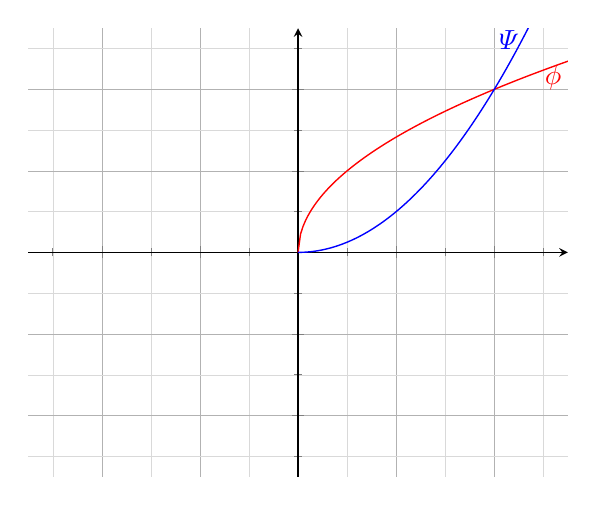
\begin{tikzpicture}
		\begin{axis}[
				xmin = -5.5, xmax = 5.5, ymin = -5.5, ymax = 5.5, 
				grid = both, axis lines = middle, 
				grid style={line width=.1pt, draw=gray!30}, 
				xticklabels={,,},
				yticklabels={,,},
				minor tick num=1,
				major grid style={line width=.2pt, draw=gray!60} 
			]
			\addplot[name path=xaxis, draw=none, domain=0:26,samples=10]{0};
			\addplot[name path=yaxis, draw=none, ] coordinates{(0.0, 4.0) (4.0, 4.0)};
			\addplot[name path=phi, line width=0.5pt,domain=0.0:25.5,samples=500, mark=none,color=red]{2.0 * sqrt(x)};
			\addplot[name path=psi, line width=0.5pt,domain=0.0:25.5,samples=500, mark=none,color=blue]{ 0.25 * x*x };
			\draw (axis cs:5.2,4.3) node[color=red] {$\phi$};
			\draw (axis cs:4.3,5.2) node[color=blue] {$\varPsi$};
		\end{axis}
		\end{tikzpicture}
	}
	~
	\resizebox{0.3\textwidth}{!}{
		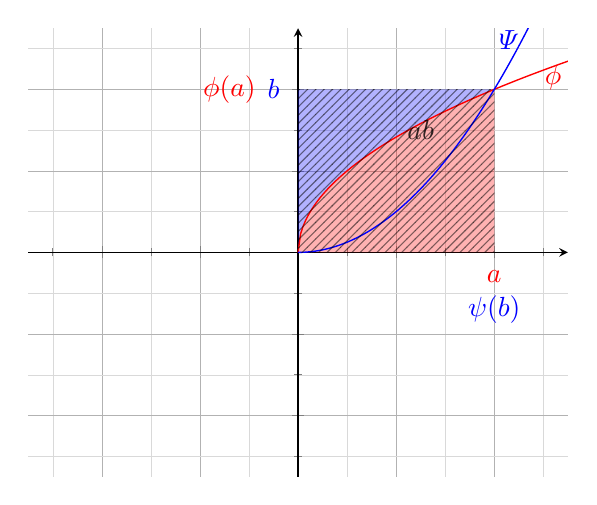
\begin{tikzpicture}
		\begin{axis}[
				xmin = -5.5, xmax = 5.5, ymin = -5.5, ymax = 5.5, 
				grid = both, axis lines = middle, 
				grid style={line width=.1pt, draw=gray!30}, 
				xticklabels={,,},
				yticklabels={,,},
				minor tick num=1,
				major grid style={line width=.2pt, draw=gray!60} 
			]
			\addplot[name path=xaxis, draw=none, domain=0:26,samples=10]{0};
			\addplot[name path=yaxis, draw=none, ] coordinates{(0.0, 4.0) (4.0, 4.0)};
			\addplot[name path=phi, line width=0.5pt,domain=0.0:25.5,samples=500, mark=none,color=red]{2.0 * sqrt(x)};
			\addplot[name path=psi, line width=0.5pt,domain=0.0:25.5,samples=500, mark=none,color=blue]{ 0.25 * x*x };
			\draw (axis cs:5.2,4.3) node[color=red] {$\phi$};
			\draw (axis cs:4.3,5.2) node[color=blue] {$\varPsi$};
			\addplot[fill=red ,opacity=0.3]fill  between[of=phi and xaxis, soft clip={domain=0:4}];
			\addplot[fill=blue,opacity=0.3]fill  between[of=phi and yaxis, soft clip={domain=0:4.0}];
			\draw (axis cs:4,-.6) node[color=red] {$a$};
			\draw (axis cs:-.5,4) node[color=blue] {$b$};
			\draw (axis cs:-1.4,4) node[color=red ] {$\phi(a)$};
			\draw (axis cs:4,-1.4) node[color=blue] {$\psi(b)$};
			\draw[fill, pattern=north east lines, pattern color=black, draw=none,opacity=0.5] (axis cs:0,0) rectangle (axis cs:4,4);
			\draw (axis cs:2.5,3) node[color=black,opacity=0.8] {$ab$};
		\end{axis}
		\end{tikzpicture}
	}
	\end{center}

\pagebreak
	\item $\psi(b) < a$: Note that this implies that $\phi(a) > b$, and so (using both facts), 
	$\Phi(a) - \Phi(\psi(b)) > b(a - \psi(b))$. 

	$ab = \Phi(\psi(b)) + \Psi(b) + b(a - \psi(b))$
	\begin{center}
	\resizebox{0.28\textwidth}{!}{
	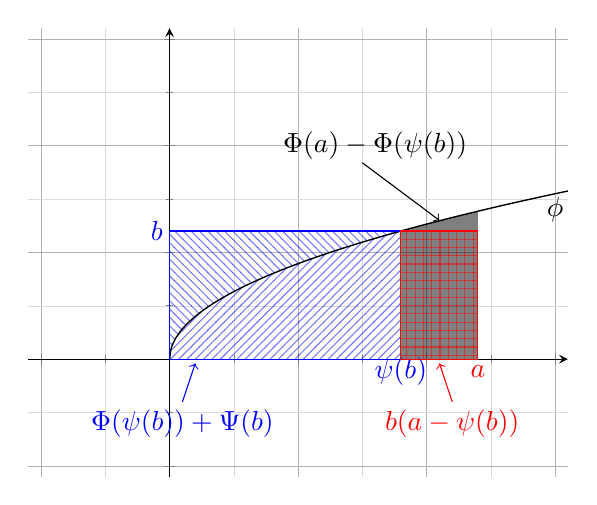
\begin{tikzpicture}
	\begin{axis}[
			xmin = -5.5, xmax = 15.5, ymin = -5.5, ymax = 15.5, 
			grid = both, axis lines = middle, 
			grid style={line width=.1pt, draw=gray!30}, 
			xticklabels={,,},
			yticklabels={,,},
			minor tick num=1,
			major grid style={line width=.2pt, draw=gray!60} 
		]
		\addplot[name path=xaxis, draw=none, domain=0:26,samples=10]{0};
		\addplot[name path=yaxis, draw=none, ] coordinates{(0.0, 6.0) (9.0, 6.0)};
		\addplot[name path=phi,line width=0.5pt,domain=0.0:25.5,samples=500,mark=none,color=black]{2.0 * sqrt(x)};
		%
		\draw (axis cs:15,7.0) node[color=black] {$\phi$};
		\draw (axis cs:12,-.6) node[color=red] {$a$};
		\draw (axis cs:-.5,6) node[color=blue] {$b$};
		\draw (axis cs:9,-.6) node[color=blue] {$\psi(b)$};
		%
		\addplot [dashed,color=blue] coordinates { (9, 6) (9, 0) };
		\addplot[pattern=north west lines, pattern color=blue,opacity=0.5] fill between[of=yaxis and phi,soft clip={domain=0:9}];
		\addplot[pattern=north east lines, pattern color=blue,opacity=0.5] fill between[of=phi and xaxis,soft clip={domain=0:9}];
		\addplot[color=black,opacity=0.5] fill between[of=phi and xaxis,soft clip={domain=9:12}];
		\draw[fill,pattern=grid, pattern color=red,opacity=0.5] (axis cs:9,0) rectangle (axis cs:12,6);
		\draw[fill=none,color=blue] (axis cs:0,0) rectangle(axis cs:9,6);
		\draw[fill=none,color=red] (axis cs:9,0) rectangle(axis cs:12,6);
		%
		\draw (axis cs:0.5,-3) node[color=blue] {$\Phi(\psi(b)) + \Psi(b)$};
		\draw (axis cs:11.0,-3) node[color=red] {$b(a - \psi(b))$};
		\draw (axis cs:8.0,10) node[color=black] {$\Phi(a) - \Phi(\psi(b))$};
		\draw [->, blue  ] (axis cs:0.5, -2) -- (axis cs:1.0, -.2);
		\draw [->, red   ](axis cs:11.0, -2) -- (axis cs:10.5, -.2);
		\draw [->, black ](axis cs:7.5, 9.2) -- (axis cs:10.5, 6.5);
	\end{axis}
	\end{tikzpicture}
	}
	~
	\resizebox{0.28\textwidth}{!}{
	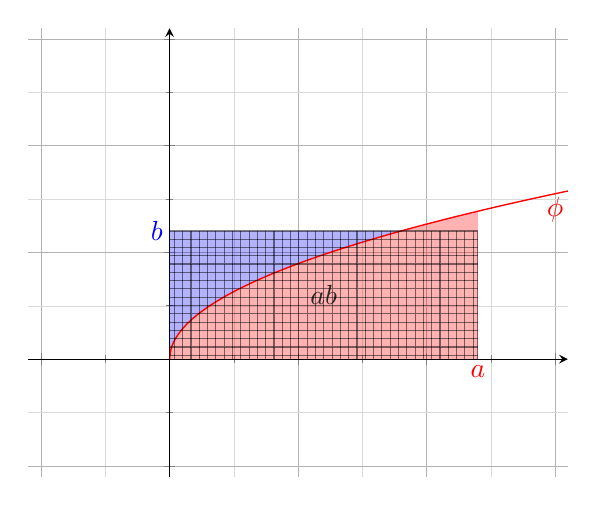
\begin{tikzpicture}
	\begin{axis}[
			xmin = -5.5, xmax = 15.5, ymin = -5.5, ymax = 15.5, 
			grid = both, axis lines = middle, 
			grid style={line width=.1pt, draw=gray!30}, 
			xticklabels={,,},
			yticklabels={,,},
			minor tick num=1,
			major grid style={line width=.2pt, draw=gray!60} 
		]
		\addplot[name path=xaxis, draw=none, domain=0:26,samples=10]{0};
		\addplot[name path=yaxis, draw=none, ] coordinates{(0.0, 6.0) (9.0, 6.0)};
		\addplot[name path=phi,line width=0.5pt,domain=0.0:25.5,samples=500,mark=none,color=red]{2.0 * sqrt(x)};
		\draw (axis cs:15,7.0) node[color=red] {$\phi$};
		\addplot[fill=red ,opacity=0.3]fill between[of=phi and xaxis,soft clip={domain=0:12}];
		\addplot[fill=blue,opacity=0.3]fill between[of=phi and yaxis,soft clip={domain=0:9.0}];
		\draw (axis cs:12,-.6) node[color=red] {$a$};
		\draw (axis cs:-.5,6) node[color=blue] {$b$};
		\draw[fill,pattern=grid,pattern color=black,opacity=0.5] (axis cs:0,0) rectangle (axis cs:12,6);
		\draw (axis cs:6,3) node[color=black,opacity=0.8] {$ab$};
	\end{axis}
	\end{tikzpicture}
	}
	\end{center}

	\item $\psi(b) > a$: Note that this implies that $\phi(a) < b$, and so (similarly to the case above), 
	$\Psi(b) - \Psi(\phi(a)) > a(b - \phi(a))$. 

	\begin{center}
	\resizebox{0.27\textwidth}{!}{
	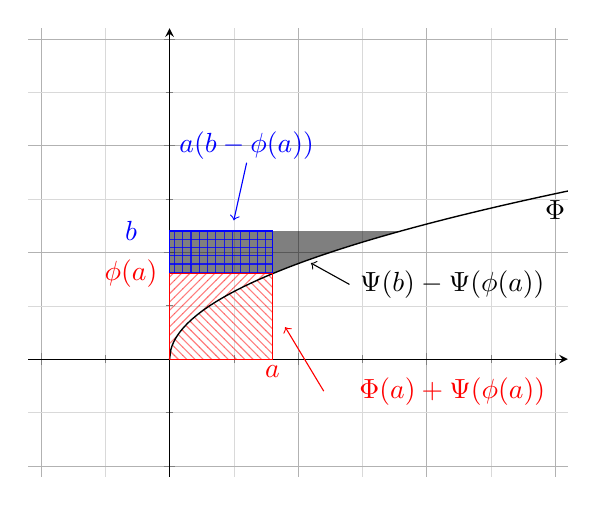
\begin{tikzpicture}
	\begin{axis}[
			xmin = -5.5, xmax = 15.5, ymin = -5.5, ymax = 15.5, 
			grid = both, axis lines = middle, 
			grid style={line width=.1pt, draw=gray!30}, 
			xticklabels={,,},
			yticklabels={,,},
			minor tick num=1,
			major grid style={line width=.2pt, draw=gray!60} 
		]
		\addplot[name path=xaxis, draw=none, domain=0:26,samples=10]{0};
		\addplot[name path=yaxis, draw=none, ] coordinates{(0.0, 6.0) (9.0, 6.0)};
		\addplot[name path=yaxis2, draw=none, ] coordinates{(0.0, 4.0) (4.0, 4.0)};
		\addplot[name path=psi, line width=0.5pt,domain=0.0:25.5,samples=500, mark=none,color=black]{ 2.0 * sqrt(x)};%0.25 * x*x };
		%
		\draw (axis cs:15.0,7) node[color=black] {$\Phi$};
		\draw (axis cs:4,-.6) node[color=red] {$a$};
		\draw (axis cs:-1.5,6) node[color=blue] {$b$};
		\draw (axis cs:-1.5,4) node[color=red] {$\phi(a)$};
		%
		\addplot[color=black,opacity=0.5] fill between[of=yaxis and psi,soft clip={domain=4:9}];
		\draw[fill, color=black, opacity=0.5] (axis cs:0,4) rectangle(axis cs:4, 6);
		\addplot[pattern = north east lines, pattern color=red,opacity=0.5] fill between[of=yaxis2 and psi,soft clip={domain=0:4}];
		\addplot[pattern = north west lines, pattern color=red,opacity=0.5] fill between[of=xaxis and psi,soft clip={domain=0:4}];
		\draw[fill, pattern=grid, pattern color=blue, opacity=0.8] (axis cs:0,4) rectangle (axis cs:4,6);
		\draw[fill=none,color=blue] (axis cs:0,4) rectangle(axis cs:4,6);
		\draw[fill=none,color=red] (axis cs:0,0) rectangle(axis cs:4,4);
		%
		\draw (axis cs:11.0,-1.5)node[color=red  ] {$\Phi(a) + \Psi(\phi(a))$};
		\draw (axis cs:3.0,10   )node[color=blue ] {$a(b - \phi(a))$};
		\draw (axis cs:11.0, 3.5)node[color=black] {$\Psi(b) - \Psi(\phi(a))$};
		\draw [->, red   ] (axis cs: 6 ,-1.5) -- (axis cs:4.5, 1.5);
		\draw [->, blue  ] (axis cs:3.0, 9.2) -- (axis cs:2.5, 6.5);
		\draw [->, black ] (axis cs: 7 , 3.5) -- (axis cs:5.5, 4.5);
	\end{axis}
	\end{tikzpicture}
	}
	~
	\resizebox{0.27\textwidth}{!}{
	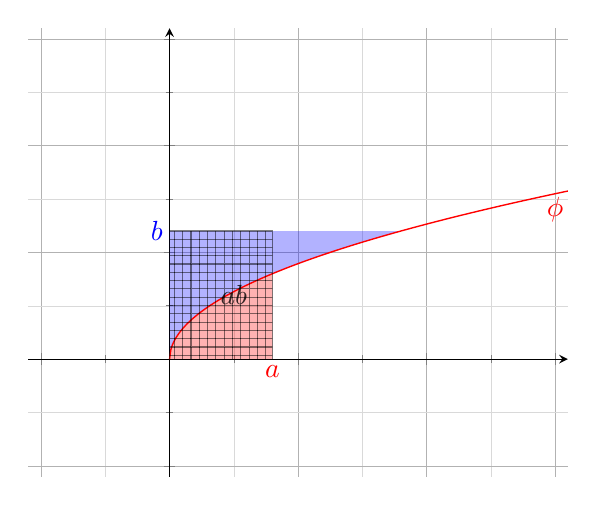
\begin{tikzpicture}
	\begin{axis}[
			xmin = -5.5, xmax = 15.5, ymin = -5.5, ymax = 15.5, 
			grid = both, axis lines = middle, 
			grid style={line width=.1pt, draw=gray!30}, 
			xticklabels={,,},
			yticklabels={,,},
			minor tick num=1,
			major grid style={line width=.2pt, draw=gray!60} 
		]
		\addplot[name path=xaxis, draw=none, domain=0:26,samples=10]{0};
		\addplot[name path=yaxis, draw=none, ] coordinates{(0.0, 6.0) (9.0, 6.0)};
		\addplot[name path=phi, line width=0.5pt,domain=0.0:25.5,samples=500, mark=none,color=red]{2.0 * sqrt(x)};
		\draw (axis cs:15,7.0) node[color=red] {$\phi$};
		\addplot[fill=red ,opacity=0.3]fill  between[of=phi and xaxis, soft clip={domain=0:4}];
		\addplot[fill=blue,opacity=0.3]fill  between[of=phi and yaxis, soft clip={domain=0:9.0}];
		\draw (axis cs:4,-.6) node[color=red] {$a$};
		\draw (axis cs:-.5,6) node[color=blue] {$b$};
		\draw[fill, pattern=grid, pattern color=black, opacity=0.5] (axis cs:0,0) rectangle (axis cs:4,6);
		\draw (axis cs:2.5,3) node[color=black,opacity=0.8] {$ab$};
	\end{axis}
	\end{tikzpicture}
	}
	\end{center}
	\end{itemize}
\end{proof}
\end{pblm}

\begin{pblm}\label{p:130}%130 
	Let $p > 1$. If $\phi(x) = x^{p-1}$, then the preceding inequality takes the form 
	\begin{equation*}
		ab \le \frac{1}{p}a^p + \frac{1}{q}b^q
	\end{equation*}
	where $q$ is the number such that $\frac{1}{p} + \frac{1}{q} = 1$. Equality holds if 
	and only if $b = a^{p-1}$ or equivalently iff $b^q = a^p$. 
\begin{proof}
	Let $\Phi(a) = \int_0^ax^{p-1}$, $\Psi(a) = \int_0^ax^{\frac{1}{p-1}}$. Then by \mPref{p:129},
	\begin{equation*}
	\begin{array}{rcl}
		ab & \le & \Phi(a) + \Psi(b) \\
		& = & \int_0^a x^{p-1} + \int_0^b x^\frac{1}{p-1} \\ 
		& = & \frac{1}{p}a^p + \frac{p-1}{p}b^\frac{p-1}{p}
	\end{array}
	\end{equation*}
	Let $q = \frac{p}{p-1}$. Then 
	\begin{equation*}
		\frac{1}{p} + \frac{p-1}{p} = \frac{p}{p} = 1
	\end{equation*}
	Then $\phi(a) = b \Leftrightarrow a^{p-1} = b$
\end{proof}
\end{pblm}

\begin{pblm}%131
	Let $p > 1$ and let $q$ be so that $\frac{1}{p} + \frac{1}{q} = 1$. Let $f$ and $g$ 
	be measurable functions on a set $E$ such that $\int_E |f|^p < \infty$ and 
	$\int_E|g|^q<\infty$. Then 
	\begin{equation*}
		\int_E|fg|\le\left(\int_E|f|^p\right)^{1/p}\left(\int_E|g|^q\right)^{1/q}. 
	\end{equation*}
	In particular, the left side of the inequality is finite. Equality holds iff for some $\alpha, \beta$, 
	$\alpha|f|^p = \beta|g|^q$ a.e. on $E$ or $f = 0$ a.e. or $g=0$ a.e. \\
	{\scriptsize{(Suppose first that $\int_E|f|^p = \int_E|g|^q=1$. Apply the preceding 
	problem with $a=|f(x)|,~b=|g(x)|,~x\in E$ and integrate. For arbitrary $f$ and $g$, 
	consider $F = f/(\int_E|f|^p)^{1/p},~G=g/(\int_E|g|^q)^{1/q}$. This is H\"{o}lder's 
	Inequality. For $p = q = 2$ it is usually called the Cauchy or Cauchy-Schwarz Inequality.)}}
\begin{proof}
	Let $a = |f(x)|$, $b = |g(x)|$. Then by \mPref{p:130}, 
	$ab \le \frac{1}{p}a^p + \frac{1}{q}b^q$, and so 
	\begin{equation*}
		|fg| \le \frac{|f|^p}{p} + \frac{|g|^q}{q}
	\end{equation*}
	and so 
	\begin{equation*}
	\begin{array}{c}
		\int |fg| \le \int \frac{|f|^p}{p} + \int \frac{|g|^q}{q}\\
		\int |fg| \le \frac{1}{p}\int |f|^p + \frac{1}{q}\int |g|^q
	\end{array}
	\end{equation*}

	Now suppose that $\int |f|^p + \int|g|^q = 1$, then let 
	$F = \frac{|f|}{\left(\int_E|f|^p\right)^\frac{1}{p}}$, 
	$G = \frac{|g|}{\left(\int_E|g|^q\right)^\frac{1}{q}}$.  

	\begin{equation*}
	\begin{array}{rcl}
		FG  = \frac{|fg|}{\left(\int|f|^p\right)^\frac{1}{p}\left(\int|g|^q\right)^\frac{1}{q}} & \le & 
			\frac{|f|^p}{p\int|f|^p} + \frac{|g|^q}{q\int|g|^q} = \frac{F^p}{p} + \frac{G^q}{q}\\
		\frac{1}{\left(\int|f|^p\right)^\frac{1}{p}\left(\int|g|^q\right)^\frac{1}{q}}\int |fg| & \le & 
			\frac{1}{p\int|f|^p}\int|f|^p + \frac{1}{q\int|g|^q}\int |g|^q
	\end{array}
	\end{equation*}


	Equal if and only if: 
	
	\noindent ($\Rightarrow$) Let 
	$\int_E|fg| = \left(\int_E|f|^p\right)^\frac{1}{p}\left(\int_E|g|^q\right)^\frac{1}{q}$, 
	and assume for contradiction that 
	$\forall \alpha, \beta$, $\alpha|f|^p \neq \beta|g|^q$. Then 
	\begin{equation*}
		\frac{1}{\int_E|f|^p}|f|^p \neq \frac{1}{\int_E|g|^q}|g|^q 
	\end{equation*}
	So 
	\begin{equation*}
		F^p \neq G^q
	\end{equation*}
	which implies that 
	\begin{equation*}
	\begin{array}{rcl}
		\int|FG| &<& \int \left(\frac{|F|^p}{p} + \frac{|G|^q}{q}\right)\\
		\int 1 &<& \int 1
	\end{array}
	\end{equation*}
	which is a contradiction. 

	\noindent ($\Leftarrow$) Now, let $\alpha, \beta$ be such that $\alpha|f|^p = \beta|g|^q$, and 
	it is not the case that $\alpha = \beta = 0$. 

	Then $|f|^p = \frac{\beta}{\alpha}|g|^q$, which implies that 
	$|f| = \left(\frac{\beta}{\alpha}\right)^\frac{1}{p}|g|^\frac{q}{p}$. 
	So 
	\begin{equation*}
	\begin{array}{lccc}
		\int_E|fg| = & \left(\frac{\beta}{\alpha}\right)^\frac{1}{p}\int_E|g|^\frac{q}{p}|g| & \le & 
		\left(\frac{\beta}{\alpha}\right)^\frac{1}{p}\left(\int|g|^q\right)^\frac{1}{p} 
		\left(\int|g|^q\right)^\frac{1}{q}\\
		& \verteq & & \verteq \\
		& \left(\frac{\beta}{\alpha}\right)^\frac{1}{p}\int|g|^q & = & \left(\frac{\beta}{\alpha}\right)^\frac{1}{p}\int|g|^q. 
	\end{array}
	\end{equation*}
%%%%%%%%%%%%%%%%%%%%%%%%%%%%%%%%%%%%%%%%%%%%%%%%%%%%%%%%%%%%%%%%%%%%%%%%%%%%%%%%%%%%%%%%%%%
\end{proof}
\end{pblm}

\begin{pblm}%132
	Let $p > 1$. If $\int_E|f|^p<\infty$ and $\int_E|g|^p<\infty$ then $\int_E|f+g|^p<\infty$ 
	and 
	\begin{equation*}
		\left(\int_E|f+g|^p\right)^{1/p} \le \left(\int_E|f|^p\right)^{1/p} + 
					\left(\int_E|g|^p\right)^{1/p}.
	\end{equation*}
	{\scriptsize{(For the first assertion, for any $x \in E$, 
	\begin{equation*}
	\begin{array}{rcl}
		|f(x)+g(x)|^p & \le &  (2\max\{|f(x)|,|g(x)|\})^p\\
				& \le & 2^p\max\{|f(x)|^p,|g(x)|^p\} 
				\le 2^p(|f(x)|^p + |g(x)|^p). 
	\end{array}
	\end{equation*}
	Then show $|f+g|^p \le |f+g|^{p-1}|f|+|f+g|^{p-1}|g|$ and apply H\"{o}lder's Inequality 
	where you use $q(p - 1) = p$. The result of this problem is called Minkowski's Inequality.)
	}}
\begin{proof}
	First of all,  $|f+g|^p = |f+g|^p|f+g|^{p-1} \le |f||f+g|^{p-1} + |g||f+g|^{p-1}$ 
	and so for $q = \frac{p}{p - 1}$ (which gives $q(p-1) = p$), 
	\begin{equation*}
	\begin{array}{rcccc}
		|f+g|^p  & \le & |f||f+g|^{p-1} & + & |g||f+g|^{p-1}\\
		\int |f+g|^p  & \le & \underbrace{\int|f+g|^{p-1}\int|f|}_{\vertle} & + & 
					\underbrace{\int|f+g|^{p-1}\int|g|}_{\vertle}\\
			&  & \left(\int(|f+g|^{p-1})^q\right)^\frac{1}{q}\left(\int|f|^p\right)^\frac{1}{p} & + & 
			     \left(\int(|f+g|^{p-1})^q\right)^\frac{1}{q}\left(\int|g|^p\right)^\frac{1}{p}\\
			& & \verteq & & ~~ \verteq \\
			&  & \left(\int(|f+g|^p\right)^\frac{1}{q}\left(\int|f|^p\right)^\frac{1}{p} & + & 
			     \left(\int(|f+g|^p\right)^\frac{1}{q}\left(\int|g|^p\right)^\frac{1}{p}\\
		\left(\int|f+g|^p\right)^{1-\frac{1}{q}} & \le & 
				\left(\int|f|^p\right)^\frac{1}{p} & + & \left(\int|g|^p\right)^\frac{1}{p}\\
		\left(\int|f+g|^p\right)^{\frac{1}{p}} & \le & 
				\left(\int|f|^p\right)^\frac{1}{p} & + & \left(\int|g|^p\right)^\frac{1}{p}
	\end{array}
	\end{equation*}
\end{proof}
\end{pblm}

\begin{defn}%133
	A measurable function $f$ on a set $E$ is \textbf{essentially bounded} if its 
	\textbf{essential supremum} 
	\begin{equation*}
		\|f\|_\infty = \inf\{M: |f(x)| \le M a.e.\}
	\end{equation*}
	is finite. Note that if $f$ is continuous on $E$, then $\|f\|_\infty=\sup\{|f(x)|:x\in E\}$ . 
\end{defn}

\begin{pblm}%134
	If $f$ is a measurable function on a set $E$ such that $\|f\|_\infty$ is finite, then 
	there is a subset $A$ of $E$ such that $m(A) = 0$ and $|f(x)| \le \|f\|_\infty$ for all 
	$x \in E\setminus A$. \\
	{\scriptsize{(If not, then for some $n$, there is $B, m(B) > 0$ and $|f(x)|\ge\|f\|_\infty + \frac{1}{n}$ 
	on $B$.)}}
\begin{proof}
	Suppose otherwise. That is, suppose $\|f\|_{\infty}$ is finite and there is no desired subset $A$. Let $B$ be a subset of $E$ such that $|f(x)|>\|f\|_{\infty}$. Then by our hypothesis, $m(B)>0$ (since $\|f(x)\| \leq \|f\|_{\infty}$ for all $x \in E\setminus B$). 
	
	Moreover, there exists $n$ such that for all $x \in B$, $|f(x)| \geq \|f\|_{\infty} + 1/n$. But $B$ has nonzero measure, so $\|f\|_{\infty}$ is not the $\inf$, which is a contradiction.
\end{proof}
\end{pblm}

\begin{pblm}%135
	If $\|f\|_\infty$ and $\|g\|_\infty$ are finite, then $\|f+g\|_\infty$ is finite and 
	$\|f+g\|_\infty \le \|f\|_\infty+\|g\|_\infty$. 
\begin{proof}
	Since for all real $f$, $g$, $|f + g| \le |f|+|g|$, 
	\begin{equation*}
		\inf\{M: |f(x) + g(x)| \le M ~ a.e.\} \le \inf\{M:|f(x)| \le M ~ a.e.\} + \inf\{M: |g(x)| \le M ~ a.e.\} 
	\end{equation*}
	and since $\|f\|_\infty < \infty$ and $\|g\| < \infty$, $\|f + g\|_\infty \le \|f\|_\infty + \|g\|_\infty < \infty$. 
\end{proof}
\end{pblm}

\begin{pblm}%136
	If $\int_E|f|<\infty$ and $\int_E|g|<\infty$, then $\int_E|f+g|\le\int_E|f|+\int_E|g|$. 
\begin{proof}
	For all real $f$, $g$,  $|f + g| \le |f| + |g|$, so $\int_E|f + g|\le \int_E|f| + \int_E|g|$
\end{proof}
\end{pblm}

\begin{rmk}%137
	We have now shown that the mapping $f\rightarrow \|f\|_p$ satisfies the triangle 
	inequality for each $p$, $1\le p\le\infty$, where $\|f\|_p = (\int_E|f|^p)^{1/p}$ 
	for $1 \le p < \infty$. These functions are, however, not quite norms on the sets of 
	functions on which they are defined because it is not true that $\|f\|_p = 0$ implies 
	that $f = 0$. What it does imply is that $f(x) = 0$ a.e. on $E$. We can fix this by 
	regarding our objects as equivalence classes of functions, where $f \sim g$ means 
	$f = g$ a.e. With this understanding we have now shown that for each $p$, 
	$1 \le p < \infty$, the set 
	\begin{equation*}
		L^p(E) = \left\{f:\int_E|f|^p < \infty \right\}
	\end{equation*}
	is a normed linear space with norm $\|f\|_p = (\int_E|f|^p)^{1/p}$. Also 
	\begin{equation*}
		L^\infty(E) = \left\{f:\|f\|_\infty < \infty \right\}
	\end{equation*}
	is a normed linear space. 
\end{rmk}

\begin{rmk}%138
	As normed linear spaces the $L^p$ spaces are metric spaces the $L^p$ spaces are 
	metric spaces with the distance function $d_p(f, g) = \|f - g\|_p$. The next big 
	question is whether they are complete with respact to this distance function. This 
	is easier for $L^\infty$ than for $L^p$ with $P < \infty$. 
\end{rmk}

\begin{pblm}%139
	The set $C[0,1]$ can be considered a subset of $L^p[0,1]$ for each $p$. It is in 
	fact dense in $L^p$ for each finite $p$ as we could see by using the problems from 
	some time ago about approximatin measurable functions by continuous functions. (It 
	is not dense in $L^\infty$ as we will see in the next problem.) Consider the sequence 
	$\{f_n\}_{n=3}^\infty$ of continuous functions defined by 
	\begin{equation*}
		f_n(x) = \left\{
		\begin{matrix}
		0, & 0 \le x \le \frac{1}{2} - \frac{1}{n}\\
		\frac{n}{2}\left(x - \frac{1}{2} + \frac{1}{n}\right), & \frac{1}{2} - \frac{1}{n} \le x \le \frac{1}{2} + \frac{1}{n}\\
		1, & \frac{1}{2} + \frac{1}{n} \le x \le 1.
		\end{matrix}
		\right.
	\end{equation*}
	\begin{enumerate}[(a)]
		\item Show that this sequence is a Cauchy sequence in $L^1[0,1]$. (Not a 
			calc problem. Draw a picture and compute area.)
		\item Show that this sequence is a Cauchy sequence in $L^p[0,1]$ for $1 < p < \infty$. 
			(Use $|f_n - f_m| < 1$ on $[0,1]$!)
		\item What is the limit $f$ of this sequence in $L^p[0,1],~1\le p<\infty$? 
			Justify your conclusion. 
	\end{enumerate}
\begin{proof}
	\begin{center}
	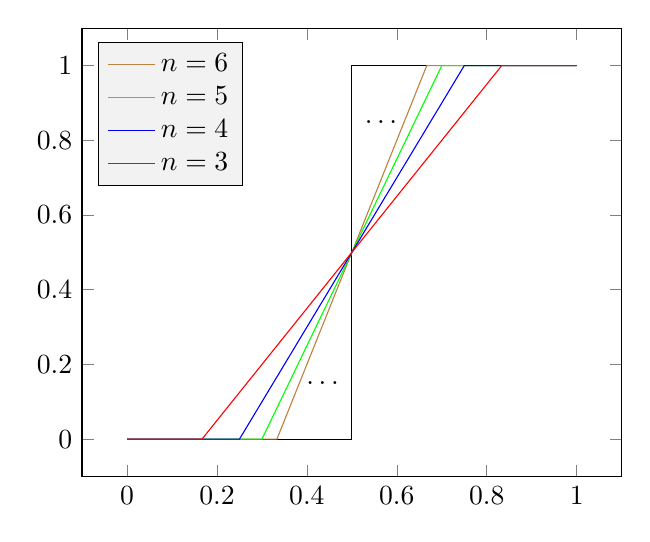
\begin{tikzpicture}
	\begin{axis}[legend pos=north west, legend style={fill=gray!10}]
		\addplot[color=black, forget plot] coordinates{
			(0,0)
			(.5, 0.0)
			(.5, 1.0)
			(1,1)
		};
		\addplot[color=brown] coordinates{
			(0,0)
			(.3333, 0.0)
			(.6666, 1.0)
			(1,1)
		};\addlegendentry{$n = 6$};
		\addplot[color=green] coordinates{
			(0,0)
			(.3, 0.0)
			(.7, 1.0)
			(1,1)
		};\addlegendentry{$n = 5$};
		\addplot[color=blue] coordinates{
			(0,0)
			(.25, 0.0)
			(.75, 1.0)
			(1,1)
		};\addlegendentry{$n = 4$};
		\addplot[color=red] coordinates{
			(0,0)
			(.166666, 0.0)
			(.833333, 1.0)
			(1,1)
		};\addlegendentry{$n = 3$};
		\draw (axis cs:0.44, 0.15) node {$\dots$};
		\draw (axis cs:0.57, 0.85) node {$\dots$};
	\end{axis}
	\end{tikzpicture}
	\end{center}
	\begin{enumerate}[(a)]
		\item For each $n$, $|f_n|_1 = \frac{1}{2}$, and $\lim\limits_{n\to\infty} |f_n| = \frac{1}{2}$  
		\item let $p \ge 1$. 
		\item the limit of the sequence in $L^p[0,1]$ for $1 \le p < \infty$
	\end{enumerate}
%%%%%%%%%%%%%%%%%%%%%%%%%%%%%%%%%%%%%%%%%%%%%%%%%%%%%%%%%%%%%%%%%%%%%%%%%%%%%%%%%%%%%%%%%%%
\end{proof}
\end{pblm}

\begin{pblm}~ %140
	\begin{enumerate}[(a)]
	\item Show that the sequence $\{f_n\}_{n=3}^\infty$ of the preceding problem is not 
		Cauchy in $L^\infty[0,1]$, or equivalently in $C[0,1]$ with the uniform norm. 
	\item Show that the limit $f$ from the preceding problem satisfies $\|f - f_n\|_\infty = 1/2$ 
		for each $n$. 
	\item Show that for any $g \in C[0,1]$, $\|f - g\|_\infty \ge 1/2$. (Thus $C[0,1]$ is not 
		dense in $L^\infty[0,1]$.)
	\end{enumerate}
\begin{proof}
	~
	\begin{enumerate}[(a)]
	\item 
	\item 
	\item 
	\end{enumerate}
%%%%%%%%%%%%%%%%%%%%%%%%%%%%%%%%%%%%%%%%%%%%%%%%%%%%%%%%%%%%%%%%%%%%%%%%%%%%%%%%%%%%%%%%%%%
\end{proof}
\end{pblm}

\begin{pblm} %141
	$L^\infty(E)$ is a Banach space. 
	%\\
	%{\scriptsize{(Let $\{f_n\}_{n=1}^\infty$ be a Cauchy sequence in $L^\infty(E)$ and choose a representative 
	%of each $f_n$, which we still denote by $f_n$. For each positive integer $k$ there is $n_k$ 
	%so that $\|f_n - f_m\|_\infty < 2^{-k}$ whenever $m, n \ge n_k$. Consider the sequence 
	%$\{f_{nk}\}_{k=1}^\infty$. Then $\ell > k$ implies $\|f_{n\ell}-f_{nk}\|<2^{-k}$. There is 
	%a set $A$, $m(A) = 0$, such that the series $f_{n_1}(x) + \sum\limits_{i=2}^k(f_{n_i}(x)-f_{n_{i-1}}(x))$ 
	%of real numbers converges absolutely for each $x\in E\setminus A$. The function $f$ defined as 
	%the pointwise limit of this series is in $L^\infty(E)$. Given $\epsilon > 0$ there is 
	%$n_\epsilon$ so that $m, n \ge n_\epsilon$ implies that $\|f_n - f_m\|_\infty < \epsilon$. Then 
	%for any such $f_m$ and any $x \in E\setminus A$, $|f(x) - f_m(x)| = 
	%\lim\limits_{k\to\infty}|f_{n_k}(x)-f_m(x)|\le\epsilon$.)}}
\begin{proof}
	We already know that $L^\infty(E)$ is a normed linear space, so all that remains to be shown 
	is that it is complete. (i.e. every Cauchy sequence converges)

	Let $\{f_n\}_{n=1}^\infty$ be a Cauchy sequence in $L^\infty(E)$, choose a representation of each 
	$f_n$, call it $f_n$. Then since $\{f_n\}_{n=1}^\infty$ is Cauchy, for any $k \in \Zp$, there is 
	a positive integer $n_k$ such that 
	\begin{equation*}
		||f_n - f_m||_\infty < \frac{1}{2^k}~~~\forall m, n \ge n_k
	\end{equation*}
	Then consider the sequence for $k > 0$ $\{f_{n_k}\}_{k=1}^\infty$. For any $l > k$, we know that 
	$||f_m - f_{n_l}||_\infty < \frac{1}{2^l} < \frac{1}{2^k}$ for all $m \ge n_l$, which implies that 
	$||f_{n_l} - f_{n_k}||_\infty < \frac{1}{2^k}$. 

	Then consider $F_k = f_{n_1} + \sum\limits_{n=2}^k (f_{n_i} - f_{n_{i-1}})$. Note that this is actually 
	another way of representing each $f_{n_k}$. Note that each $(f_{n_i} - f_{n_{i-1}})$ has 
	$||f_{n_i} - f_{n_{i-1}}||_\infty < \frac{1}{2^{i-1}}$, so 
	\begin{equation*}
		||F_{k+1} - F_k||_\infty < \frac{1}{2^k} ~~~\forall k
	\end{equation*}
	And furthermore, $||F_k||_\infty < ||f_{n_1}||_\infty + 1$ for all $k$. 
	So $F_k$ converges absolutely a.e., and if we define 
	\begin{equation*}
		\lim\limits_{k\to\infty}F_k = f
	\end{equation*}
	Then this is a bounded function a.e., and so $f \in L^\infty(E)$. 

	Now we need to show that $\{f_n\}_{n=1}^\infty$ converges to $f$. This is a Cauchy sequence, so 
	for any $\epsilon > 0$, there is $n_\epsilon$ such that for all $m, n \ge n_\epsilon$, 
	\begin{equation*}
		||f_n - f_m||_\infty < \epsilon
	\end{equation*}
	so for any such $f_m$, 
	\begin{equation*}
		|f(x) - f_m(x)| = \lim\limits_{n\to\infty}|f_{n_k}(x) - f_m(x)| \le \epsilon. 
	\end{equation*}
	So $\{f_n\} \rightarrow f$ a.e. and $f \in L^\infty(E)$ for any Cauchy sequence inf $L^\infty(E)$. 
	Thus $L^\infty(E)$ is a complete (and therefore Banach) space. 
\end{proof}
\end{pblm}

\begin{pblm}%142
	For each $1\le p < \infty$, if $\{f_n\}_{n=1}^\infty$ is a Cauchy sequence in $L^p(E)$ and 
	if we choose a representative of each $f_n$ (we will still denote these functions by $\{f_n\}$), 
	then there is a subsequence $\{f_{n_k}\}_{k=1}^\infty$ that converges pointwise a.e. on $E$ to 
	a measurable function $f$ such that $\int_E|f|^p < \infty$. 
	%{\scriptsize{(For each positive integer $k$ there 
	%is $n_k$ so that $\|f_n - f_m\|_p < 2^{-k}$ whenever $m,n \ge n_k$. Why? Consider the sequence 
	%$\{f_{n_k}\}_{k=1}^\infty$. Then $\ell > k$ implies $\|f_{n_\ell} - f_{n_k}\|_p < 2^{-k}$. 
	%For each integer $k \ge 2$, set $g_k = |f_{n_1}| + \sum\limits_{i=2}^k|f_{n_i} - f_{n_{i-1}}|$. 
	%Then $\{g_k\}_{k=1}^\infty$ is a non-decreasing sequence of non-negative functions such that 
	%$\|g_k\|_p \le \|f_{n_1}\|_p + 1$ for each $k$, and the extended real-valued function 
	%$g(x) = \lim\limits_{k\to\infty}g_k(x)$ satisfies $\int_Eg^p = \lim\limits_{k\to\infty}\int_Eg^p_k < \infty$. 
	%For almost all $x \in E$, the series $f_{n_1}(x) + \sum\limits_{i=2}^\infty(f_{n_i}(x) - f_{n_{i-1}}(x))$ 
	%of real numbers converges absolutely, and so defines a measurable  function $f$ there. This 
	%function is in $L^p(E)$.)}}
\begin{proof}
	Let $1 \le p < \infty$. Then if $\{f_n\}_{n=1}^\infty$ is Cauchy, then for any $k \in \Zp$, 
	there is $n_k$ such that 
	\begin{equation*}
		||f_n - f_m||_p , \frac{1}{2^k} ~~ \forall m, n \ge n_k
	\end{equation*}

	Now consider the subsequence $\{f_{n_k}\}_{k=1}^\infty$ of $\{f_n\}$. As in the 
	previous problem, for any $l > k$, $||f_{n_l} - f_{n_k}||_\infty < \frac{1}{2^k}$. 
	Now, for each $k \ge 2$, let 
	\begin{equation*}
		g_k(x) = |f_{n_1}| + \sum\limits_{i=2}^k|f_{n_i} - f_{n_{i-1}}|
	\end{equation*}
	Then $\{g_k\}_{k=2}^\infty$ is non-decreasing, non-negative, and 
	since for each $k$, $|g_k| \le |f_{n_1}| + 1$, then 
	\begin{equation*}
		||g_k||_p \le ||f_{n_1}||_p + 1
	\end{equation*}
	for each $k$, and setting $g = \lim\limits_{k\to\infty}g_k$, we have 
	\begin{equation*}
		\int_Eg^p = \lim\limits_{k\to\infty}\int_Eg^p_k < \infty
	\end{equation*}

	This sequence converges absolutely, and if we let 
	\begin{equation*}
		f = \lim\limits_{k\to\infty}\left\{f_{n_1} + \sum\limits_{i=2}^k(f_{n_i} - f_{n_i - 1})\right\}
	\end{equation*}
	then we know that this sequence converges absolutely, and as each term $f_k$ is bounded by $g_k$, we have 
	$|f| \le g$ which implies that 
	\begin{equation*}
		\int_E|f|^p \le \int_Eg^p < \infty
	\end{equation*}
	and so $f$ is in $L^p(E)$. 
\end{proof}
\end{pblm}

\begin{pblm}%143
	If $\{f_n\}_{n=1}^\infty$ and $f$ are as in the preceding problem, then $f_n \rightarrow f$ in 
	$L^p(E)$. Thus $L^p(E)$ is complete.\\
	{\scriptsize{(Let $\epsilon > 0$ be given. For $m,n > n_\epsilon$ Then Fatou's Lemma implies 
	$ \int_E|f-f_m|^p \le \lim\inf\limits_{k}\int_E|f_{n_k} - f_m|^p < \epsilon^p.) $ }}
\begin{proof}
	Let $\{f_n\}_{n=1}^\infty$ and $f$ be as in the previous problem. Then since $\{f_n\}$ is 
	Cauchy, for any $\epsilon > 0$, 
	\begin{equation*}
		||f_n - f_m||_p < \epsilon ~~~ m, n \ge n_\epsilon
	\end{equation*}
	so by Fatou's Lemma (\mPref{p:fatou}), 
	\begin{equation*}
		\int_E |f - f_m|^p \le \lim\inf\limits_{k}\int_E|f_{n_k} - f_m|^p 
				= \lim\inf\limits_{k}||f_{n_k} - f_m||_p < \epsilon^p
	\end{equation*}
	and so the sequence $\{f_n\}_{n=1}^\infty$ converges to $f$. 
\end{proof}
\end{pblm}

\begin{rmk}%144
	The completeness of $L^p$ is sometimes referred to as the Riesz-Fischer Theorem, although 
	what Riesz actually proved in 1906 was rather different. It was similar to the example 
	explored below. 
\end{rmk}

\begin{rmk}%145
	There is another way to arrange the proof of the completeness of $L^p$ that looks a little 
	slicker, but perhaps changes the perception of what's really going on. One proves the abstract 
	theorem that a normed linear space $X$ is complete if and only if the following property is 
	true: if a series $\sum\limits_{n=1}^\infty x_n$ \textbf{converges absolutely} (this means 
	that the series $\sum\limits_{n=1}^\infty \|x_n\|$ of norms converges in $\R$) then the series 
	converges in $X$ (this means that the sequence of partial sums $\sum\limits_{n=1}^N x_n$ 
	converges to an element of $X$). Then you show that $L^p(E)$ has this property. If you look 
	carefully, you will find these elements in what we did.
\end{rmk}

\begin{defn}%146
	The set $\ell^p$ (read ``little $L^p$'') is the set of real (or complex) sequences $\{c_n\}_{n=1}^\infty$ 
	such that $\sum\limits_{n=1}^\infty |c_n|^p < \infty$. It is a complete normed linear space-a 
	Banach space-with the norm 
	\begin{equation*}
		\|\{c_n\}\|_p = \left(\sum\limits_{n=1}^\infty |c_n|^p\right)^{1/p}. 
	\end{equation*}
	(That this is a norm with respect to which $\ell^p$ is complete can be proved by methods 
	roughly similar to what we have done.)
\end{defn}

\begin{rmk}%147
	We can add more structure for $L^2$ and $\ell^2$. An \textbf{inner product} on a vector 
	space is a map $(\cdot , \cdot): V \times V \rightarrow \R$ with the properties 
	\begin{enumerate}
	\item $(v,v) \ge 0$ and $(v, v) = 0$ iff $v = 0$ (zero element in $V$, of course), 
	\item $(v,w) = (w,v)$ for all $v, w\in V$, 
	\item $(av + bw, u) = a(v,u) + b(w, u)$ for all $u, v, w \in V$ and all $a, b \in \R$. 
	\end{enumerate}
	Given an inner product, $\|v\| = \sqrt{(v,v)}$ is a norm on $V$, so every inner product 
	space is a normed linear space and hence a metric space. (Topology from algebra!) If it is 
	complete as a metric space, we call it a \textbf{Hilbert space}. However in an inner product 
	space we can also define the angle between elements by analogy with the dot product. In 
	particular $v$ and $w$ are \textbf{orthogonal} if $(v,w) = 0$. It is possible to extend 
	``dot product geometry'' to this context-orthogonal bases, expressing an arbitrary element 
	as the sum of its projections onto the elements of an orthogonal basis and so forth. The so 
	forth includes the equivalent of the Pythagorean Theorem: the square of the norm of an element 
	is the sum of the squares of the lengths of its projections. However the extension must 
	cope with the fact that bases are typically countably infinite sets, so the sums are infinite 
	sums and there are questions of convergence.

	In $\ell^2$ the inner product is $(\{c_n\}, \{d_n\}) = \sum\limits_{n=1}^\infty c_nd_n$. The 
	equivalent of H\"{o}lder's Inequality guarantees that $|(\{c_n\},\{d_n\})| \le \|\{c_n\}\|\|\{d_n\}\|$ 
	and so in particular that the sum converges absolutely. In $L^2(E)$ the inner product is 
	$(f,g) = \int_Efg$. Again this converges by H\"{o}lder's Inequality. 

	In $L^2[0,\pi]$ the sequence $\{\sin nx\}_{n=1}^\infty$ has the properties 
	$\|\sin nx\|_2 = \sqrt{\frac{\pi}{2}}$ and $\sin nx \perp \sin mx$ if $m \neq n$, that is, 
	$\int_0^\pi \sin nx \sin mx dx = 0$ if $m neq n$. The projection of any function $f \in L^2[0,\pi]$ 
	on $nx$ is 
	\begin{equation*}
		\frac{(f,\sin nx)}{(\sin nx, \sin nx)}\sin nx = 
		\left(\frac{2}{\pi}\int_0^\pi f(t) \sin nt dt\right)\sin nx. 
	\end{equation*}
	The projection $p_n$ of $f \in L^2[0,\pi]$ on SPAN$\{\sin x, \sin 2x, \dots \sin nx\}$ is 
	$\sum\limits_{k=1}^n c_k\sin kx$ where $c_k = \frac{2}{\pi}\int_0^\pi f(t) \sin kl dt$. It is 
	easy to see, using the orthogonality of the different sine functions that $\|p_n\|_2^2 = 
	\sum\limits_{k=1}^nc_k^2 \le \|f\|_2^2$ where the last inequality just comes from the fact that 
	any projection of $f$ has norm less than or equal to that of $f$. It follows that $\{c_k\}_{k=1}^\infty$ 
	is in $\ell^2$, that $\{p_n\}_{n=1}^\infty$ is Cauchy in $L^2[0,\pi]$ (since $\|p_n - p_m\|_2^2 = 
	\sum\limits_{k=m+1}^nc_k^2$), and then by completeness that $\{p_n\}_{n=1}^\infty$ converges 
	in $L^2[0,\pi]$ to an element $\sum\limits_{k=1}^\infty c_k\sin kx$. It turns out that 
	$f = \sum\limits_{k=1}^\infty c_k \sin kx$ and that 
	\begin{equation*}
		\|f\|_2^2 = \sum\limits_{k=1}^\infty c_k^2  = \|\{c_n\}\|^2. 
	\end{equation*}
	(These turn out to be equivalent to the statement that the only element of $L^2[0,\pi]$ that 
	is orthogonal to every $\sin nx$ is the zero element, that is, the set $\{\sin nx\}_{n=1}^\infty$ 
	is \textbf{complete} (roughly, large enough to function as a basis).)

	The result of all of this is that the mapping $f\rightarrow \{c_n\}$ is an isometry (linear 
	mapping preserving the norm) of $L^2[0,\pi]$ onto $\ell^2$. In particular, given any 
	sequence in $\ell^2$, there is an $L^2$ function $f$ with that sequence of Fourier sine coefficients. 
	This is approximately the content of the original Riesz-Fischer Theorem in 1906.
\end{rmk}

\end{document}
